\documentclass[a4paper, 12pt]{book}
%\documentclass[a4paper, 12pt, draft]{book}  Nalogo preverite tudi z opcijo draft, ki vam bo pokazala, katere vrstice so predolge!



\usepackage[utf8x]{inputenc}   % omogoča uporabo slovenskih črk kodiranih v formatu UTF-8
\usepackage[slovene,english]{babel}    % naloži, med drugim, slovenske delilne vzorce
\usepackage[pdftex]{graphicx}  % omogoča vlaganje slik različnih formatov
\usepackage{fancyhdr}          % poskrbi, na primer, za glave strani
\usepackage{amssymb}           % dodatni simboli
\usepackage{amsmath}           % eqref, npr.
\usepackage[hyphens]{url}  % dodal Solina
\usepackage{comment}       % dodal Solina

\usepackage[pdftex, colorlinks=true,
						citecolor=black, filecolor=black, 
						linkcolor=black, urlcolor=black,
						pagebackref=false, 
						pdfproducer={LaTeX}, pdfcreator={LaTeX}, hidelinks]{hyperref}

\usepackage{color}       % dodal Solina
\usepackage{soul}       % dodal Solina

%%%%%%%%%%%%%%%%%%%%%%%%%%%%%%%%%%%%%%%%
%	DIPLOMA INFO
%%%%%%%%%%%%%%%%%%%%%%%%%%%%%%%%%%%%%%%%
\newcommand{\ttitle}{Mobilna aplikacija Asana Master}
\newcommand{\ttitleEn}{Asana Master mobile application}
\newcommand{\tsubject}{\ttitle}
\newcommand{\tsubjectEn}{\ttitleEn}
\newcommand{\tauthor}{Klementina Garbajs}
\newcommand{\tkeywords}{Joga, mobilna aplikacija, Expo, React Native}
\newcommand{\tkeywordsEn}{Yoga, mobile app, Expo, React Native}


%%%%%%%%%%%%%%%%%%%%%%%%%%%%%%%%%%%%%%%%
%	HYPERREF SETUP
%%%%%%%%%%%%%%%%%%%%%%%%%%%%%%%%%%%%%%%%
\hypersetup{pdftitle={\ttitle}}
\hypersetup{pdfsubject=\ttitleEn}
\hypersetup{pdfauthor={\tauthor, kg4597@student.uni-lj.si}}
\hypersetup{pdfkeywords=\tkeywordsEn}

%%%%%%%%%%%%%%%%%%%%%%%%%%%%%%%%%%%%%%%%
% postavitev strani
%%%%%%%%%%%%%%%%%%%%%%%%%%%%%%%%%%%%%%%%  

\addtolength{\marginparwidth}{-20pt} % robovi za tisk
\addtolength{\oddsidemargin}{40pt}
\addtolength{\evensidemargin}{-40pt}

\renewcommand{\baselinestretch}{1.3} % ustrezen razmik med vrsticami
\setlength{\headheight}{15pt}        % potreben prostor na vrhu
\renewcommand{\chaptermark}[1]%
{\markboth{\MakeUppercase{\thechapter.\ #1}}{}} \renewcommand{\sectionmark}[1]%
{\markright{\MakeUppercase{\thesection.\ #1}}} \renewcommand{\headrulewidth}{0.5pt} \renewcommand{\footrulewidth}{0pt}
\fancyhf{}
\fancyhead[LE,RO]{\sl \thepage}
\fancyhead[RE]{\sc \tauthor}              % dodal Solina
\fancyhead[LO]{\sc Diplomska naloga}     % dodal Solina


\newcommand{\BibTeX}{{\sc Bib}\TeX}

%%%%%%%%%%%%%%%%%%%%%%%%%%%%%%%%%%%%%%%%
% naslovi
%%%%%%%%%%%%%%%%%%%%%%%%%%%%%%%%%%%%%%%%  


\newcommand{\autfont}{\Large}
\newcommand{\titfont}{\LARGE\bf}
\newcommand{\clearemptydoublepage}{\newpage{\pagestyle{empty}\cleardoublepage}}
\setcounter{tocdepth}{1}	      % globina kazala

%%%%%%%%%%%%%%%%%%%%%%%%%%%%%%%%%%%%%%%%
% konstrukti
%%%%%%%%%%%%%%%%%%%%%%%%%%%%%%%%%%%%%%%%  
\newtheorem{izrek}{Izrek}[chapter]
\newtheorem{trditev}{Trditev}[izrek]
\newenvironment{dokaz}{\emph{Dokaz.}\ }{\hspace{\fill}{$\Box$}}

%%%%%%%%%%%%%%%%%%%%%%%%%%%%%%%%%%%%%%%%%%%%%%%%%%%%%%%%%%%%%%%%%%%%%%%%%%%%%%%
%% PDF-A
%%%%%%%%%%%%%%%%%%%%%%%%%%%%%%%%%%%%%%%%%%%%%%%%%%%%%%%%%%%%%%%%%%%%%%%%%%%%%%%


%%%%%%%%%%%%%%%%%%%%%%%%%%%%%%%%%%%%%%%% 
% define medatata
%%%%%%%%%%%%%%%%%%%%%%%%%%%%%%%%%%%%%%%% 
\def\Title{\ttitle}
\def\Author{\tauthor, kg4597@student.uni-lj.si}
\def\Subject{\ttitleEn}
\def\Keywords{\tkeywordsEn}

%%%%%%%%%%%%%%%%%%%%%%%%%%%%%%%%%%%%%%%% 
% \convertDate converts D:20080419103507+02'00' to 2008-04-19T10:35:07+02:00
%%%%%%%%%%%%%%%%%%%%%%%%%%%%%%%%%%%%%%%% 
\def\convertDate{%
    \getYear
}

{\catcode`\D=12
 \gdef\getYear D:#1#2#3#4{\edef\xYear{#1#2#3#4}\getMonth}
}
\def\getMonth#1#2{\edef\xMonth{#1#2}\getDay}
\def\getDay#1#2{\edef\xDay{#1#2}\getHour}
\def\getHour#1#2{\edef\xHour{#1#2}\getMin}
\def\getMin#1#2{\edef\xMin{#1#2}\getSec}
\def\getSec#1#2{\edef\xSec{#1#2}\getTZh}
\def\getTZh +#1#2{\edef\xTZh{#1#2}\getTZm}
\def\getTZm '#1#2'{%
    \edef\xTZm{#1#2}%
    \edef\convDate{\xYear-\xMonth-\xDay T\xHour:\xMin:\xSec+\xTZh:\xTZm}%
}

\expandafter\convertDate\pdfcreationdate 

%%%%%%%%%%%%%%%%%%%%%%%%%%%%%%%%%%%%%%%%
% get pdftex version string
%%%%%%%%%%%%%%%%%%%%%%%%%%%%%%%%%%%%%%%% 
\newcount\countA
\countA=\pdftexversion
\advance \countA by -100
\def\pdftexVersionStr{pdfTeX-1.\the\countA.\pdftexrevision}


%%%%%%%%%%%%%%%%%%%%%%%%%%%%%%%%%%%%%%%%
% XMP data
%%%%%%%%%%%%%%%%%%%%%%%%%%%%%%%%%%%%%%%%  
\usepackage{xmpincl}
\includexmp{pdfa-1b}

%%%%%%%%%%%%%%%%%%%%%%%%%%%%%%%%%%%%%%%%
% pdfInfo
%%%%%%%%%%%%%%%%%%%%%%%%%%%%%%%%%%%%%%%%  
\pdfinfo{%
    /Title    (\ttitle)
    /Author   (\tauthor, kg4597@student.uni-lj.si)
    /Subject  (\ttitleEn)
    /Keywords (\tkeywordsEn)
    /ModDate  (\pdfcreationdate)
    /Trapped  /False
}


%%%%%%%%%%%%%%%%%%%%%%%%%%%%%%%%%%%%%%%%%%%%%%%%%%%%%%%%%%%%%%%%%%%%%%%%%%%%%%%
%%%%%%%%%%%%%%%%%%%%%%%%%%%%%%%%%%%%%%%%%%%%%%%%%%%%%%%%%%%%%%%%%%%%%%%%%%%%%%%

\begin{document}
\selectlanguage{slovene}
\frontmatter
\setcounter{page}{1} %
\renewcommand{\thepage}{}       % preprecimo težave s številkami strani v kazalu
\newcommand{\sn}[1]{"`#1"'}                    % dodal Solina (slovenski narekovaji)

%%%%%%%%%%%%%%%%%%%%%%%%%%%%%%%%%%%%%%%%
%naslovnica
 \thispagestyle{empty}%
   \begin{center}
    {\large\sc Univerza v Ljubljani\\%
      Fakulteta za računalništvo in informatiko}%
    \vskip 10em%
    {\autfont \tauthor\par}%
    {\titfont \ttitle \par}%
    {\vskip 3em \textsc{DIPLOMSKO DELO\\[5mm]         % dodal Solina za ostale študijske programe
VISOKOŠOLSKI STROKOVNI ŠTUDIJSKI PROGRAM\\ PRVE STOPNJE\\ RAČUNALNIŠTVO IN INFORMATIKA}\par}%
    \vfill\null%
    {\large \textsc{Mentor}: doc.\ dr.  Mira Trebar\par}%
    {\vskip 2em \large Ljubljana, 2021 \par}%
\end{center}
% prazna stran
%\clearemptydoublepage      % dodal Solina (izjava o licencah itd. se izpiše na hrbtni strani naslovnice)

%%%%%%%%%%%%%%%%%%%%%%%%%%%%%%%%%%%%%%%%
%copyright stran
\thispagestyle{empty}
\vspace*{8cm}

\noindent
{\sc Copyright}. 
Rezultati diplomske naloge so intelektualna lastnina avtorja in Fakultete za računalništvo in informatiko Univerze v Ljubljani.
Za objavo in koriščenje rezultatov diplomske naloge je potrebno pisno privoljenje avtorja, Fakultete za računalništvo in informatiko ter mentorja.

\begin{center}
\mbox{}\vfill
\emph{Besedilo je oblikovano z urejevalnikom besedil \LaTeX.}
\end{center}
% prazna stran
\clearemptydoublepage

%%%%%%%%%%%%%%%%%%%%%%%%%%%%%%%%%%%%%%%%
% stran 3 med uvodnimi listi
\thispagestyle{empty}
\vspace*{4cm}

\noindent
Fakulteta za računalništvo in informatiko izdaja naslednjo nalogo:
\medskip
\begin{tabbing}
\hspace{32mm}\= \hspace{6cm} \= \kill

Tematika naloge:
\end{tabbing}
V diplomskem delu zasnujte mobilno aplikacijo za osebno vadbo joge. Omogoča naj ogled in izvajanje položajev, spremljanje napredka zastavljenih ciljev z beleženjem posameznih aktivnosti in občutkov ter shranjevanjem zapiskov in posnetkov. Predlagano rešitev implementirajte v ogrodju Expo z React Native in v okviru izbranega mobilnega operacijskega sistema Android predstavite njeno uporabo ter podajte nadaljnje možnosti razvoja.
\vspace{15mm}

\vspace{2cm}

% prazna stran
\clearemptydoublepage

% zahvala
\thispagestyle{empty}\mbox{}\vfill\null\it%
\noindent
Na tem mestu zapišite, komu se zahvaljujete za izdelavo diplomske naloge. Pazite, da ne boste koga pozabili. Utegnil vam bo zameriti. Temu se da izogniti tako, da celotno zahvalo izpustite.
\rm\normalfont

% prazna stran
\clearemptydoublepage

%%%%%%%%%%%%%%%%%%%%%%%%%%%%%%%%%%%%%%%%
% kazalo
\pagestyle{empty}
\def\thepage{}% preprecimo tezave s stevilkami strani v kazalu
\tableofcontents{}

% prazna stran
\clearemptydoublepage

%%%%%%%%%%%%%%%%%%%%%%%%%%%%%%%%%%%%%%%%
% seznam kratic

\chapter*{Seznam uporabljenih kratic}  % spremenil Solina, da predolge vrstice ne gredo preko desnega roba

\noindent\begin{tabular}{p{0.1\textwidth}|p{.4\textwidth}|p{.4\textwidth}}    % po potrebi razširi prvo kolono tabele na račun drugih dveh!
  {\bf kratica} & {\bf angleško} & {\bf slovensko} \\ \hline
  {\bf IDE} & {\bf integrated development enviroment} & {\bf integrirano razvojno okolje} \\ \hline
  {\bf API} & {\bf integrated development enviroment} & {\bf integrirano razvojno okolje} \\ \hline
%  \dots & \dots & \dots \\
\end{tabular}


% prazna stran
\clearemptydoublepage

%%%%%%%%%%%%%%%%%%%%%%%%%%%%%%%%%%%%%%%%
% povzetek
\addcontentsline{toc}{chapter}{Povzetek}
\chapter*{Povzetek}

\noindent\textbf{Naslov:} \ttitle
\bigskip

\noindent\textbf{Avtor:} \tauthor
\bigskip

%\noindent\textbf{Povzetek:} 
\noindent 
Asane oz. položaji imajo v jogi velik pomen, zato je pomembno, da je izvajanje le teh pravilno in v skladu z zmožnostmi posameznika. Prav z namenom učenja pravilne izvedbe položajev, spremljanjem napredka in sledenja lastnim občutkom, smo razvili mobilno aplikacijo za Android, ki je primerna tako za začetne kot nadaljevalne praktikante, saj so Asane razdeljene na različne stopnje, prav tako pa si praktikant lahko sam določi svoje cilje, katerim lahko sledi, objavi sliko napredka in ustvarja zapiske oz. dnevnik občutkov. Aplikacija je razvita z uporabo ogrodja React Native in odprtokodno platformo Expo.

\bigskip

\noindent\textbf{Ključne besede:} \tkeywords.
% prazna stran
\clearemptydoublepage

%%%%%%%%%%%%%%%%%%%%%%%%%%%%%%%%%%%%%%%%
% abstract
\selectlanguage{english}
\addcontentsline{toc}{chapter}{Abstract}
\chapter*{Abstract}

\noindent\textbf{Title:} \ttitleEn
\bigskip

\noindent\textbf{Author:} \tauthor
\bigskip

%\noindent\textbf{Abstract:} 
\noindent 

For dissertation, we decided to develop the Asana Master mobile application, which would completely bypass the journey of individuals through his Yoga paths. Asanas or  positions are of great importance in Yoga, so it is important to perform them correctly and in accordance with the abilities of individuals. In order to learn the correct execution of positions, monitor progress and the last last feeling of practitioners, we have developed an application that is suitable for both initial and advanced practices, as the Asanas are divided into different stages, and the practitioner can set their own goals.
\bigskip

\noindent\textbf{Keywords:} \tkeywordsEn.
\selectlanguage{slovene}
% prazna stran
\clearemptydoublepage

%%%%%%%%%%%%%%%%%%%%%%%%%%%%%%%%%%%%%%%%
\mainmatter
\setcounter{page}{1}
\pagestyle{fancy}

\chapter{Uvod}
Joga je za veliko ljudi le oblika sprostitve, način napajanja z energijo, vadba za boljše počutje. Za tiste, ki se z njo ukvarjajo bolj intenzivno, pa je predvsem izjemno, do potankosti izdelano in premišljeno urjenje osebnosti, ki lahko človeku omogoči, da dozori. Joga je pot k sebi. Nima pa joga le pozitivnih učinkov na um, temveč tudi na telo. 
Z leti postane naše telo manj gibčno, utrujeno, bolj občutljivo in nagnjeno k poškodbam, kar pa lahko učinkovito odpravimo z vadbo joge, saj telo postane prožnejše, bolj gibljivo in močnejše. Joga so telesni položaji ali asane preko katerih začutimo in spoznavamo svoje telo, ga nadzorujemo in izboljšujemo, vendar praksa asan ne sme biti brezglava in pretirana, zato je poznavanje položajev in pravilne izvedbe le-teh zelo pomembno. 
In kaj je asana? Sanskrtski izraz asana pomeni poza ali položaj telesa. Asana je psiho-somatska vaja za telo in um, saj z njo vplivamo tako na počutje telesa, kot tudi uma. Pozorni moramo biti tako na pravilen položaj telesa, kot tudi na naše dihanje. 

Prav z namenom pravilnega izvajanja položajev in enostavnim spremljanjem napredka, smo se za diplomsko nalogo odločili razviti Android mobilno aplikacijo Asana Master, ki bi bodočim joga učiteljem in tudi vsem ostalim omogočala lažje in bolj zabavno obliko učenja, ter dodatno motivacijo za napredek. Uporabnik ima  možnost učenja o različnih položajih v jogi, možnost spremljanja programa za izboljšanje gibljivosti, inverzij, itd., prav tako pa ima možnost ob tem še spremljati svoj lasten napredek, si podati samooceno o lastnem napredku in izraziti svoje občutke preko zapiskov.

Aplikacija je razvita z uporabo ogrodja React Native in odprtokodno platformo Expo. Za pisanje kode so bili uporabljeni jeziki, Java Script, TypeScript in SQL. Aplikacija teče na Expovem lokalnem strežniku, za povezavo do baze podatkov pa skrbi strežnik Express. Podatki so shranjeni v bazi, ki je nameščena na lokalnem strežniku MySQL.


\chapter{Pregled področja}
\label{ch0}

\section{Joga}
"Joga združuje načine zavedanja, zaznavanja, doživljanja, soočanja, spoznavanja in delovanja, preko katerih je človek zmožen bivati neodvisno od lastne pogojenosti" ~\cite{oJogi}.
Beseda joga izhaja iz korena besede yuj, ki pomeni združiti, povezati. Nakazuje na to, da se s tehnikami joge osvobodimo vezi in omogočimo združitev duše z absolutnim zavedanjem. Skozi čas se je razvila vrsta raznih praks in zvrsti joge. Nekatere izmed praks imajo s klasično jogo vedno manj skupnega, saj je po tradiciji učenje joge zahtevalo preučevanje tekstov ter pridobivanje znanja s pomočjo guruja, dan danes pa je več poudarka na izvajanju položajev in na splošnem fizičnem aspektu joge. Obstaja več različnih poti joge, ki se med seboj dopolnjujejo. Posameznik izbere pot, ki je najbližja njegovemu trenutnemu stanju zavedanja. Glavne poti so štiri: Karma joga (pot nesebičnega delovanja za dobro drugih in sveta), Jnana joga (pot modrosti in intelektualnega raziskovanja), Bhakti joga (pot predanosti in ljubezni do izbranega ideala) in Raja joga (kraljevska pot joge, ki jo sestavlja osem krakov, skozi katere se poda posameznik na poti do samorealizacije). Poleg naštetih poti obstajajo še nekatere druge, med njimi je tudi Hatha joga, katero najpogosteje srečamo na zahodu, saj daje povzornost predvsem izvajanju asan in pranajame.\\ 

\section{Zgodovina joge}
Zibelka joge naj bi bila indska civilizacija, nekje v letih od 2600 do 1900 pr. n. št., ko je joga kot posebna metoda preseganja človeške pogojenosti, omenjena v vedskih spisih, ki so nastali na območju današnje Indije ~\cite{prirocnik}. Preden se je joga uveljavila kot osebna praksa, so kot prevladujoči načini samo-preseganja služili obredni rituali žrtvovanja. Preko teh ritualov so si ljudje skušali zagotoviti moč nadzora nad lastno minljivostjo. S prihodom nomadskih plemen na območje indske civilizacije pa so obredni rituali začeli izgubljati svojo vlogo in začelo se je vedsko obdobje, ki je trajalo nekje od leta 1700 do 1100 pr. n. št. V tem času se je znanje o jogi prenašalo preko ustnega izročila, šele na začetku 2. tisočletja n. š. pa je bilo znanje zapisano v Vede. Vede veljajo za ene najstarejših besedil sveta in predstavljajo osrednje bistvo duhovnosti, hinduizma in temelje joge.

S koncem Vedskega obdobja teče začetek Asketskih praks, ki so izvor jogijskih praks. Asketi so popolnoma zavračili avtoriteto Ved in pomembnost ritualov. To odobje je trajalo od 6. do 3. stol. pr. n. št., za tem pa je sledilo obdobje Upanišad. Zmožnost odrešitve je v tem času prenehala obstajati kot privilegij pogoej s spoznavanjem ritualnih praks, saj se je pozornost preusmerila na osebi in njen način bivanja. Rishiji - modreci in avtorji upanišadskih spisov so začeli poudarjati, da je odrešitev zmožen doseči vsak z načinom svojega bivanja in delovanja.  To bivanje in delovanje so opisali v "samkhyah", iz katerih izhaja tudi teoretični princip joge. Ta temelji na predpostavki, da je človeško trpljenje posledia nepoznavanja sebe in vzrokov svojih dejanj. Zaradi neznanja se Sebstvo identificira s fizičnim telesom. Rešitev je možna šele, ko se Sebstvo osvobodi teh napačnih poistovetenj in materialnih vezi. S tem, ko je možen bivati onstran fizičnega in psihičnega izkustva, lahko spoznava in spreminja pogoje bivanja in vzroke svojega delovanja. 

Filozofija joge je prevzela osnovne predpostavke "samkhye", le da odrešitve ne povezuje toliko s spoznanjem, kolikor z načinom delovanja. Človek je zmožen preseči lastno pogojenost in bivati neodvisno od materialnega sveta (za katerega se je predpostavljajo, da vsebuje tako fizično kot psihično realnost) prav z določenim načinom doživljanja in delovanja v materialnem svetu. Omenjen način doživljanja in delovanja je v filozofiji joge opisan kot jogijska praksa.

Prvo sistematično zbirko jogijskih praks, ki so se izvajale na območju današnje Indije je izdelal Patanjali v svojih Yoga-sutrah, prvem samostojnem besedilu o jogi, v katerih avtor opredeli osmeročleno pot joge~\cite{ZgodovinaJoge}. Besedilo je eno glavnih jogijskih besedil na katerega se lahko opre novodoben praktikant joge. V njih Patanjali predstavi skupek navodil, ki jih mora praktikant izvajati istočasno in v celoti, če želi napredovati po poti joge. Vrednote etike in morale praktikant skrbno in počasi integrira v svoje življenje.

Tradicionalno jogo sestavlja osem temeljnih vej Raja joge (ash – osem, anga – veja) in obsegajo vse vidike telesnega, čustvenega in mentalnega življenja. Osem vej je sistematično opisanih v Yoga-sutrah:

\begin{enumerate}
	\item \textbf{Yama ali etične zmožnosti}: navodila kako naj jogi deluje v odnosu do sveta s poudarkom na samodisciplino in vzdržnost.
		\begin{itemize}
			\item nenasilje (ahimsa) – nezmožnost škodovati sebi in drugim
			\item resnicoljubnost (satya) – usklajenost govora z dejanji
			\item onemogočanje kraje oziroma težnje po prilaščanju tega kar nam ne pripada (asteya)
			\item neodvisnost od spolnih potreb (brahmacarya)
			\item onemogočenje pohlepa (aparigraha) oziroma težnje po prilaščanju tega česar ne potrebujemo
		\end{itemize}
	
	\item \textbf{Niyama ali discipline}: navodila kako naj jogi deluje do sebe
		\begin{itemize}
			\item čistost telesa in duha (sauca)
			\item notranje zadovoljstvo ali zmožnost izkusiti zadovoljstvo neodvisno od zunanjih dejavnikov (santosha)
			\item razvoj samodispline (tapas)
			\item odsotnost besed (kastha mauna)
			\item odsotnost gest in kretenj (akara mauna)
			\item samo-preučevanje (svadhyaya)
			\item predanost božanskemu (ishvara pranidana)
		\end{itemize}

	\item \textbf{Asana ali telesni položaji}
	\item \textbf{Pranayama ali tehnike nadzora energije}
	\item \textbf{Pratyahara ali neodvisnost čutil od zaznavanja zunanjih dejavnikov}
	\item \textbf{Dharana ali zbranost in zmožnost nadzorovanega usmerjanja pozornosti na en predmet}
	\item \textbf{Dhyana ali meditacija oz. podaljšana koncentracija}
	\item \textbf{Samadhi ali stanje skupne zavesti}
\end{enumerate}


\section{Asane in njihov pomen}
Beseda asana pomeni stabilen in udoben položaj. Največkrat pa jo v slovenščini enačimo s terminom vaja ali položaj.

Praktikant želi najti optimalno naravnavo znotraj asane glede na posebnosti in sposobnosti svojega telesa. Svojo zaznavo najprej osredotoči na občutenje položaja posameznega dela telesa, ko najde varen položaj, pa v njem išče udobje in stabilnost ter poskuša zmanjšati telesni napor, da bi lahko sčasoma njegova pozornost prešla od fizične zaznave.

V hatha jogi so asane ena osnovnih tehnik telesnega gibanja~\cite{Asane}. Asane dajejo telesu gibljivost in pravilno držo, ki je temelj pravilne izvedbe jogijskih položajev. Z njo med vadbo preprečimo morebitne mišične ali skeletne poškodbe in krepimo mišice stabilizatorje trupa. Za boljše življenje in učinkovito prakso brez bolečin, se moramo naučiti zavestnega nadzora telesne drže in zavedanja poravnave telesa v vsakem položaju.

Jogijska praksa od praktikantov ne zahteva le pravilnega izvajanja asan temveč tudi pozornost in usmerjenost uma v to, kar počnemo. V asani smo, kot pove že sanskrtsko ime "as" oz. biti, tukaj in zdaj.

Nekateri viri navajajo, da naj bi bilo asan nekje med 70 in 80 tisoč. Poimenovali so jih po živalih, rastlinah, mineralih in  božanstvih. Večina asan vsebuje hatha princip, ki pomeni princip moči. Zelo pomembno je, da asane izvajamo primerno svojim telesnim sposobnostim in pravilno, kar pomeni postopnost učenja in poslušanje svojega telesa. Nikoli ne izvajamo asan preko svojih zmožnosti, ampak le do praga bolečine. 

Izvedba asane naj bi bila stabilna in hkrati selektivno sproščena. Dihanje je sproščeno, enakomerno, pozornost je usmerjena v počutje telesa, opazujemo sporočila telesa, umirimo um in zadržujemo položaj toliko časa, dokler čutimo asano v vseh navedenih lastnostih. 

Skozi asane se nam razkrivajo naši ustaljeni psihofizični vzorci, ki jih običajno doživimo kot omejitve. V jogi ni tekmovalnosti, vsak je v svoji asani, ki trenutno ustreza njegovemu psihofizičnemu stanju. Učitelji joge pogosto pravijo, da je tista asana, ki nam je najmanj všeč, pravzaprav naša asana.

Z rednim in discipliniranim izvajanjem asan se prožnost telesa izredno poveča. Mnoge asane učinkujejo tudi terapevtsko in lahko odpravijo težave, ki nas pestijo dolgo časa in so morda videti nerešljive, odpravi pa jih lahko že pravilna drža telesa. Hkrati se poveča tudi naša prožnost duha: opazimo lahko spremembe v svojem dojemanju sveta, samozavesti, odprtosti, sposobnosti, da ocenimo položaj in ugotovimo, kaj je bistvo in kaj nepomembna navlaka. Trdno stojimo na tleh, z odprtim srcem in notranjo radostjo, ki ne potrebuje zunanjih dražljajev. Takrat smo prestopili prvo, pomembno stopnico na poti joge.
Bistvo izvajanja asane ni nujno v popolni izvedbi. Bistvo asane je v popolnem medsebojnem zavedanju duše in telesa.

\section{Sorodne aplikacije}
Pri pregledu sorodnih aplikacij smo ugotovili, da na trgu obstaja nekaj rešitev za izvajanje joge v angleškem jeziku in nekaj slovenskih prevodov.

Ena izmed boljših aplikacij, ki jo trenutno uporabljamo, je aplikacija Track Yoga ~\cite{trackyoga}, kjer ima uporabnik možnost pregleda nad različnimi asanami, prikazanimi tudi z videoposnetki, prav tako pa ima na voljo različno dolge posnetke vodene prakse oz. možnost sledenja programu, npr. programu za izboljšanje fleksibilnosti, zmanjševanju stresa, meditacija in drugo. V aplikaciji ima vsak uporabnik tudi svoj profil, kjer spremlja koliko programov in vodenih vadb je že opravil.

Ena izmed aplikacij, ki so osredotočene bolj na učenje posameznika o asanah, pa je aplikacija Yoga 108~\cite{yoga108}. V aplikaciji uporabniku ponujajo pregled nad različnimi asanami, njihovimi izgovorjavami in angleškimi prevodi, vendar pa ne ponujajo podrobnega opisa asane, njenih prednosti in prikaza pravilne izvedbe z videoposnetkom.

Obstaja seveda tudi veliko drugih aplikacij, ki pa so vse bolj ali manj osredotočene le na to, da uporabnika vodijo pri vadbi joge in ponujajo različne programe z videoposnetki, katerim potem posameznik sledi in prakticira jogo, a lahko uporabnik te aplikacije le pasivno uporablja. Zgoraj naštete aplikacije nimajo možnosti delanja zapiskov in ne omogočajo spremljanja lastnega napredka, kot je objavljanje slik, podajanje samoocene in interaktivno sledenje programu, kar uporabnika še bolj motivira.

\chapter{Načrtovanje aplikacije}
\label{ch1}

Razvoj mobilnih aplikacij ne bi smel biti več tako osredotočen le na eno glavno funkcionalnost, saj počasi prihaja čas, ko smo ljudje vedno bolj zasičeni z različnimi podatki, aplikacijami in načini shranjevanja. Vedno bolj se bomo nagibali k aplikacijam, ki omogočajo večje število funkcionalnosti v enem. Z namenom, da ima uporabnik, vse kar potrebuje za sledenje lastnemu napredku, na enem mestu, smo se odločili za izdelavo mobilne aplikacije, ki bi to tudi omogočala.

\section{Struktura mobilne aplikacije}
Načrtovanje mobilne aplikacije se je začelo z izdelavo načrta strukture mobilne aplikacije,  katerega osnovni namen je začrtati osnovno postavitev vsebine (struktura, elementi na strani), še preden sledi oblikovanje, (Slika~\ref{wireframe}). V načrtu smo zasnovali zaslon za Prijavo in Registracijo, strukturo glavnega menija ter različnih podmenijev, ki se odprejo s klikom na element v glavnem meniju. Glavni strukturi podmenijev sta na sliki prikazani s puščicami iz tretje skice (desno in navzdol). Skice desno predstavljajo strukturo podmenija Asanas in Goals, skice spodaj pa strukturo podmenija Notes.

Struktura ne vsebuje podrobnosti oblikovanja – barv, tipografij, slik. Lahko se skicira zelo na hitro na listu papirja, ali pa se pripravi v digitalni obliki s pomočjo različnih programov oz. aplikacij. Za izdelavo orisa strukture je bila uporabljena spletna platforma WireframePro~\cite{WireframePro}, ki je vodilno orodje za oblikovanje načrtov uporabniškega vmesnika za spletna mesta in mobilne aplikacije. Vključuje že pripravljene komponente uporabniškega vmesnika za iOS, Android, splet, Bootstrap, WatchOS,... in ima tudi obsežno knjižnico predlog, ki uporabnikom olajša izdelavo načrtov.\\


\begin{figure}[htbp]
\begin{center}
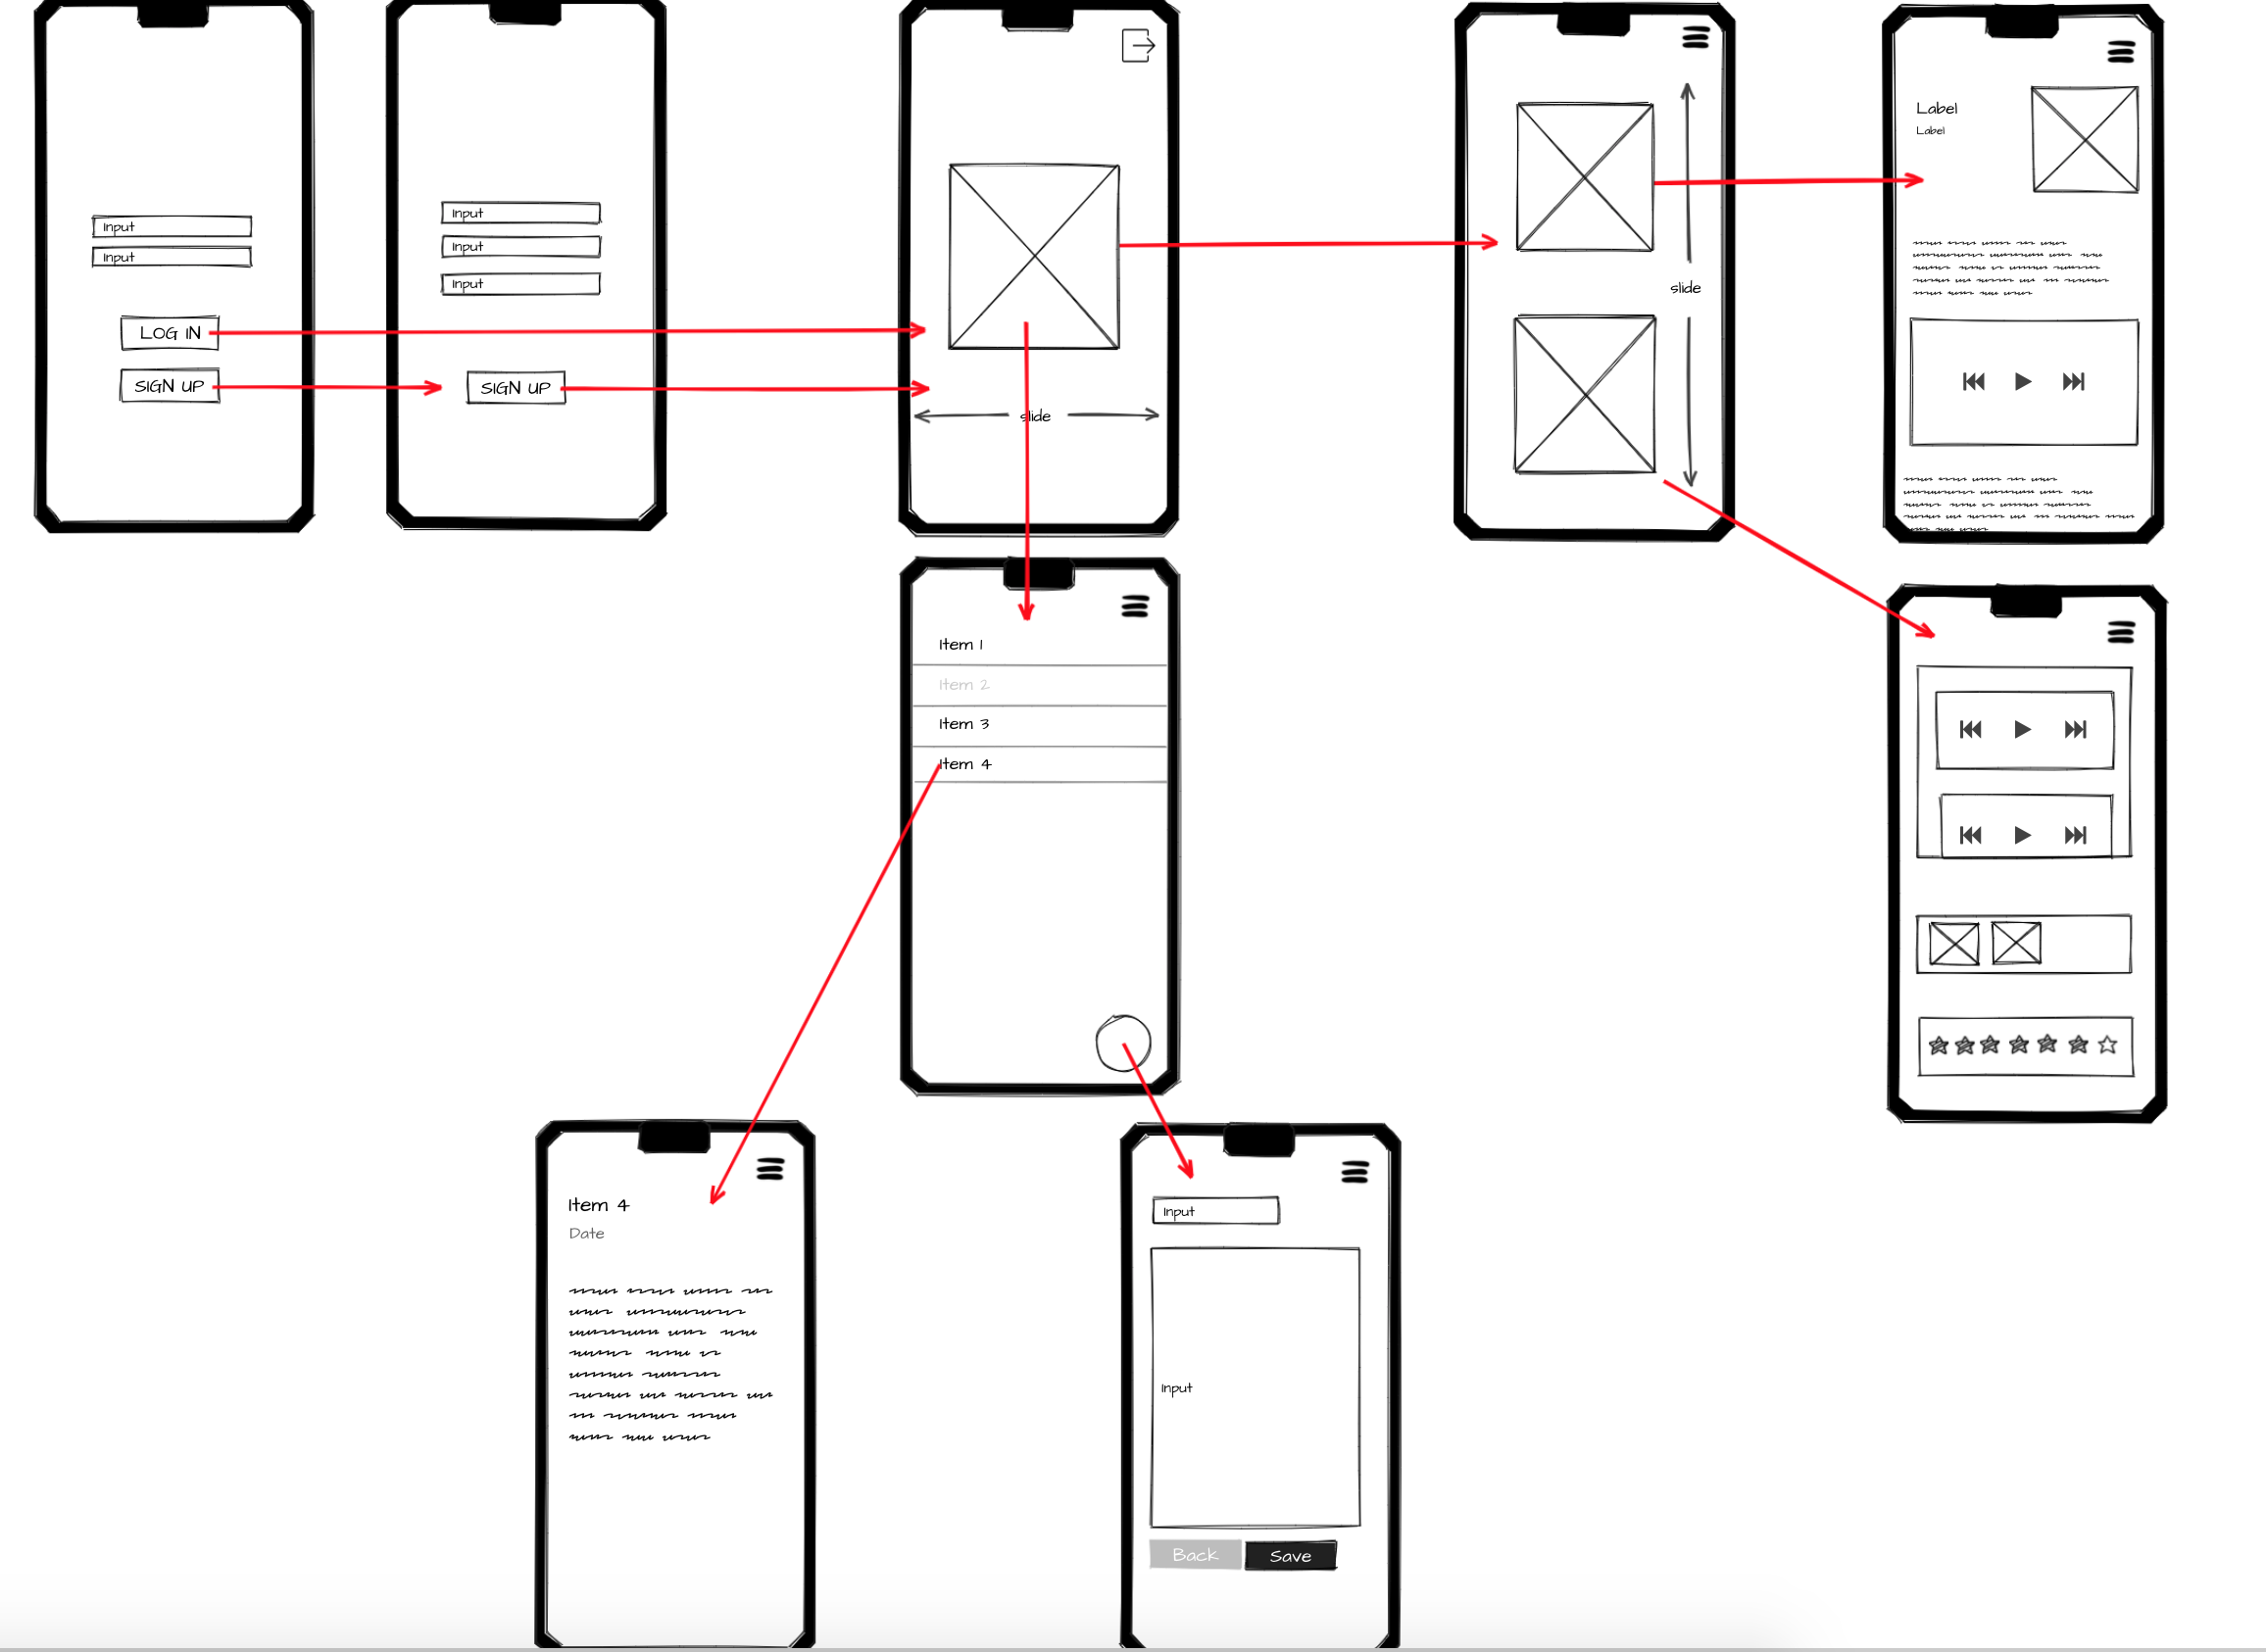
\includegraphics[scale=.35]{wireframes.png}
\end{center}
\caption{Načrt strukture mobilne aplikacije.}
\label{wireframe}
\end{figure}


\section{Arhitektura aplikacije}
Arhitektura aplikacije je sestavljena iz treh glavnih nivojev: predstavitvenega nivoja, logičnega nivoja in podatkovnega nivoja, (Slika~\ref{arh}). V predstavitvenem nivoju se nahaja grafični vmesnik oz. Android mobilna aplikacija, ki zahteva podatke iz logičnega nivoja. V logičnem nivoju se nahaja zaledni sistem (REST API), ki procesira zahtevke iz predstavitvenega nivoja in komunicira s podatkovno bazo na podatkovnem nivoju. Prednosti take arhitekture sta bolj enostavno enostavno ponovno uporabljanje dela aplikacije in integriteta podatkov~\cite{arhitektura}. Slabost pa je povečana kompleksnost dela.\\

\begin{figure}[htbp]
\begin{center}
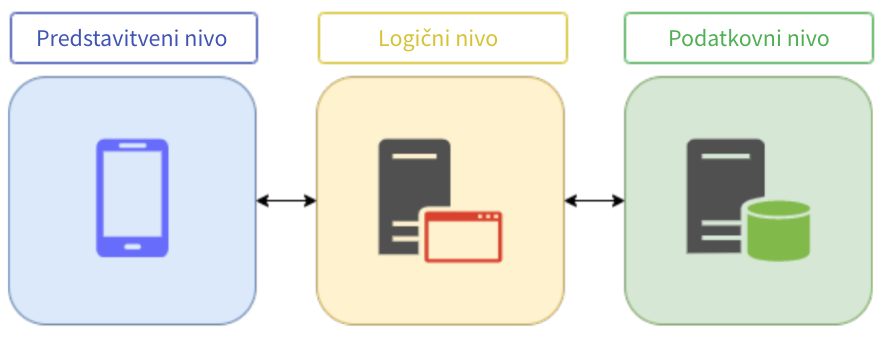
\includegraphics[scale=0.9]{arhitektura.png}
\end{center}
\caption{3-nivojska arhitektura aplikacije.}
\label{arh}
\end{figure}

\section{Funkcionalnosti aplikacije}
Glavne funkcionalnosti, ki jih ima uporabnik na voljo v aplikaciji Asana Master, so razdeljene in opisane po posameznih podmenijih v aplikaciji:

 \begin{itemize}
 \item \textbf{Prijava in registracija}:
 \begin{itemize}
   \item Registracija: kreiranje novega uporabniškega računa
  \item Prijava: prijava v mobilno aplikacijo z uporabniškim računom
 \end{itemize}

 \item \textbf{Asane}:
  \begin{itemize}
  \item Ogled položajev/asan: ogled položajev oziroma asan
  \item Ogled videoposnetkov: ogled videoposnetkov položajec v mobilni aplikaciji  
   \end{itemize}
    Podatki o asanah in jogi so vzeti in prepisani v podatkovno bazo, iz knjige The Top 100 Best Yoga Poses Relieve Stress, Increase Flexibility, and Gain Strength, avtorice Susan Hollister~\cite{yoga}. Vir nekaterih slik je tudi zgoraj omenjena knjiga, nekatere pa so bile pridobljene preko spletne strani Verywellfit~\cite{verywellfit}. Vir videoposnetkov je portal Youtube. Posnetek se predvaja neposredno v sami aplikaciji, brez dodatnega odpiranja videoposnetka izven mobilne aplikacije. Za to funkcionalnost je uporabljena React Native knjižnica react-native-youtube-iframe. Knjižnica omogoča predvajanje posnetka skozi celoten ekran mobilne naprave, s klikom na naslov posnetka pa uporabnika preusmeri na vir videoposnetka na Youtubu, kjer si ga lahko ogleda izven aplikacije.
   
\item \textbf{Goals}:
  \begin{itemize}
  \item Ocenjevanje napredka: ocenjevanje lastnega napredka uporabnika
  \item Nalaganje slik: nalaganje slik napredka uporabnika
  \item Urejanje slik: urejanje slik uporabnika
  \item Ogled slik: ogled slik napredka uporabnika 
  \item Ogled videoposnetkov programa v mobilni aplikaciji
\end{itemize}
Za nalaganje slik je uporabljena Expova knjižnica expo-image-picker, ki omogoča dostop do uporabniškega vmesnika sistema za izbiranje slik in videoposnetkov iz knjižnjice telefona ali fotografiranje s fotoaparatom. Knjižnica omogoča tudi obračanje, obrezovanje in zrcaljenje slike. 
Za ogled naloženih slik pa je uporabljena React Native knižnjica react-native-image-zoom-viewer, ki omogoča jasen in enostaven pregled slik, z dodatno možnostjo povečave slike.
Za podajanje ocene napredka je uporabljena knjižnica react-native-ratings, ki omogoča enostavno podajanje ocen v obliki zvezdic.
   
\item \textbf{Notes}:
  \begin{itemize}
  \item Kreiranje novega zapiska: uporabnik lahko kreira nov zapisek
  \item Shranjevanje novega zapiska: uporabnik lahko shrani novo ustvarjen zapisek
  \item Brisanje zapiska: uporabnik lahko željeni zapisek izbriše
  \item Ogled zapiskov: uporabnik si lahko ogleda ustvarjene zapiske
\end{itemize}
Zapiski so razdeljeni v kategorije ciljev, ter razvrščeni po dnevih. Zapiski, ki so dodani preko gumba za dodajanje zapiskov v podmeniju Notes, se shranijo pod kategorijo Random, saj niso vezani na nobenega izmed ciljev.

\end{itemize}

\chapter{Razvoj mobilne aplikacije}
\section{Uporabljena tehnologija in orodja}

Mobilna aplikacija je razvita z uporabo ogrodja React Native in ogrodja Expo, kar omogoča izdelavo mobilnih aplikacij tako za operacijski sistem Android kot iOS. Za pisanje kode so uporabljeni jeziki TypeScript, JavaScript in SQL, koda pa je napisana v programu Visual Studio Code. Za shranjevanje podatkov, je uporabljena relacijska podatkovna baza MySql, ki je povezana z lokalnim strežnikom. Podatki so shranjeni v programu TablePlus, ki omogoča enostaven vnos ter urejanje podatkov. Za prikaz podatkov iz podatkovne baze v uporabniški vmesnik skrbi Expressov API server.
Testiranje aplikacije poteka preko Expovega orodja za testiranje Expo Developer Tools. Vse spremembe v kodi, ter zgodovina spremenjenih verzij aplikacije so shranjene v programu Git.

\section{Ogrodja}
 \begin{itemize}
  \item \textbf{React Native}: React Native je JavaScript ogrodje za pisanje izvornih mobilnih aplikacij za operacijska sistema iOS in Android. Temelji na Reactu, Facebookovi JavaScript knjižnici za gradnjo uporabniških vmesnikov, a namesto na brskalnik cilja na mobilne platforme~\cite{RN}. 
React Native, je Facebook prvič izdal kot odprtokodni projekt leta 2015. V samo nekaj letih je postal ena najboljših rešitev za mobilni razvoj. React Native razvoj se uporablja za pogon nekaterih vodilnih svetovnih mobilnih aplikacij, vključno z Instagramom, Facebookom in Skypeom.
  
  \item \textbf{Expo}: Expo je ogrodje, ki se uporablja za izdelavo React Native aplikacij. Gre za nabor orodij in storitev, zgrajenih okoli React Native-a in izvornih platform, ki nam pomagajo razvijati, graditi, uvajati in hitro iterirati v iOS, Android in spletne aplikacije iz iste kodne baze JavaScript / TypeScript~\cite{EXPO}. Z uporabo Expo-ta ne potrebujemo znanja o izvorni iOS ali Android kodi, kar pomeni, da tudi uporaba orodij kot sta Xcode ali Android Studio, ni potrebna. Njegov cilj je omogočiti hiter razvoj, ne da bi morali veliko časa porabiti za vzpostavljanje razvojnega okolja. Expo ne zahteva nastavitve IDE-jev, specifičnih za platforme, kot je to v primeru React Native CLI, in ke zato celoten postopek namestitve veliko bolj enostaven. Expo prav tako ponuja okolje za testiranje Expo Developer Tools, ki omogoča enostavno testiranje aplikacij, tako na spletnem vmesniku, mobilnem simulatorju, kot tudi na mobilni napravi.
  
\item \textbf{Express}: Express je minimalno in prilagodljivo ogrodje spletnih aplikacij Node.js, ki ponuja robusten nabor funkcij tako za spletne, kot mobilne aplikacije~\cite{Express}. Z neštetimi metodami pripomočkov HTTP in vmesno programsko opremo, ki jih imamo na voljo, je omogočeno enostavno in hitro ustvarjanje robustnega API -ja.
\end{itemize}

\section{Orodja}
 \begin{itemize}
  \item \textbf{npm}: Npm je privzeti upravitelj paketov za izvajalno okolje JavaScript Node.js Namešča module, tako da jih vozlišče lahko najde, in inteligentno obvladuje konflikte med odvisnostmi~\cite{npm}. Sestavljen je iz odjemalca ukazne vrstice, imenovanega tudi npm in spletne baze javnih in plačljivih zasebnih paketov, imenovane register npm. Izjemno prilagodljiv je za podporo najrazličnejšim primerom uporabe. Najpogosteje se uporablja za objavljanje, odkrivanje, nameščanje in razvoj vozliščnih programov.
  \end{itemize}

\section{Programski jeziki}
 \begin{itemize}
  \item \textbf{Java Script}: JavaScript (krajše tudi JS) je skriptni programski jezik, katerega je razvil Netscape, da bi bil v pomoč programerjem pri izdelavi spletnih strani. Večina tistih, ki pozna vsaj nekaj osnov programiranja, ko zasliši ime JavaScript, hitro poveže s programskim jezikom Java, s katerim imata kar nekaj skupnih lastnosti~\cite{JS}. Pri skriptnih jezikih v splošnem obdelava kode traja dalje kot pri zbirnih jezikih, vendar pa so veliko bolj uporabni pri krajših programih zaradi njihove enostavnosti. Uporabnost JavaScript-a pride najbolj do izraza pri razvoju dinamičnih spletnih strani in dodajanju interaktivnosti na želeno stran.
  
  \item \textbf{TypeScript}: TypeScript je odprtokodni jezik, ki temelji na JavaScriptu, enem izmed najbolj uporabljenih jezikov na svetu, z dodajanjem statičnih definicij tipa~\cite{TS}. Tipi nam ponujajo način za opis oblike predmeta, zagotavljajo boljšo dokumentacijo in omogočajo TypeScriptu, da preveri, ali koda deluje pravilno.
Vsa veljavna koda napisana v jeziku JavaScript je tudi koda TypeScript. TypeScript se prek prevajalnika TypeScript ali Babel pretvori v JavaScript. JavaScript koda je čista in preprosta in se izvaja kjerkoli, kjer deluje JavaScript: v brskalniku, na Node.JS ali v aplikacijah.
  
  \item \textbf{SQL}: SQL je najbolj razširjen računalniški jezik, ki omogoča kreiranje, spreminjanje, branje in manipulacijo s podatki, shranjenimi v relacijski PB~\cite{SQL}. Širitev jezika gre v smeri podpore objektno relacijskim podatkovnim bazam. Jezik SQL je standardiziran (ANSI / ISO), vendar je upoštevanje standardov s strani nekaterih proizvajalcev SUPB vprašljivo. Njegove značilnosti so, da je zasnovan na množicah (ker izhaja iz relacijskega modela podatkov), ter enostaven nabor ukazov.
\end{itemize}

\section{Programi}
 \begin{itemize}
  \item \textbf{Visual Studio Code}: Za pisanje kode je uporabljen program Visual Studio Code, znan tudi kot VS Code, ki je Microsoftov brezplačen odprtokodni urejevalnik besedil. VS Code je na voljo za Windows, Linux in macOS~\cite{VSC}. Čeprav je urejevalnik razmeroma lahek, vključuje nekaj zmogljivih funkcij, zaradi katerih je VS Code v zadnjem času postalo eno najbolj priljubljenih orodij za razvojno okolje, saj podpira široko paleto programskih jezikov od Jave, C ++ in Pythona do CSS, Go in Dockerfile. Poleg tega VS Code omogoča dodajanje in celo ustvarjanje novih razširitev, vključno s kodami, iskalniki napak in podporo za razvoj v oblaku in spletnem razvoju.

 \item \textbf{MySQL}: MySQL je odprtokodni sistem za upravljanje relacijskih baz podatkov~\cite{MySQL}. Kot del široko uporabljenega svežnja tehnologij LAMP (ki ga sestavljajo operacijski sistem, ki temelji na Linuxu, spletni strežnik Apache, baza podatkov MySQL in PHP za obdelavo) se uporablja za shranjevanje in pridobivanje podatkov v najrazličnejših priljubljenih aplikacijah, spletnih mestih in storitvah.

\item \textbf{TablePlus}: Za pregledovanje in urejanje baze podatkov je bil uporabljen program TablePlus~\cite{TablePlus}. TablePlus je sodobna, izvorna aplikacija s čistim uporabniškim vmesnikom, ki razvijalcem omogoča sočasno upravljanje podatkovnih baz na zelo hiter in varen način. TablePlus podpira večino priljubljenih baz podatkov, kot so MySQL, Postgres, SQL Server, SQLite, Microsoft SQL Server, Redis, Redshift, Oracle in še veliko več.

\item \textbf{Git}: Git je brezplačen in odprtokodni porazdeljeni sistem za nadzor različic, zasnovan za hitro in učinkovito obdelavo vsega, od majhnih do zelo velikih projektov~\cite{Git}.
\end{itemize}

\section{Podatkovni nivo}
Podatkovna baza je zbirka povezanih podatkov. Prednosti uporabe podatkovne baze so možnost shranjevanja večjih količin podatkov, hitrejši prenos podatkov in hitrejša obdelava podatkov, (Slika~\ref{baza}).
Pri podatkovnem modeliranju se izvaja abstrakcija in poenostavitev nekega segmenta realnega sveta. Na osnovi modela se potem izdela podatkovna baza. Podatkovni model je povezana zbirka konceptov namenjenih opisovanju podatkov in opravljanju s podatki, ki opredeljuje sintakso in semantiko stavkov formalnega jezika. Za predstavljeno podatkovno bazo je bil uporabljen entitetno relacijski podatkovni model, ki je sestavljen iz entitet, atributov in relacij. Entiteta je v podatkovni bazi predstavljena z množico atributov. Atribut je podatkovni element, s katerim opišemo lastnost entitete. Za definiranje povezav med dvema ali več entitetami so uporabljene relacije, ki lahko pripradajo različnim entitetnim množicam. Spodaj je predstavljen fizični model s tabelami in njihovimi relacijami. Podatkovna baza je sestavljena iz petih tabel: \textit{Users}, \textit{Asanas}, \textit{Goals}, \textit{Images}, \textit{Notes}.\\

\textbf{Entitete in njihovi atributi}
  \begin{itemize}
  \item Users: id (primarni ključ), name, email, password, first{\_}login.
  \item Asanas: id (primarni ključ), name, description, image, type, name{\_}sanskrit, level, how{\_}to, video{\_}id.\\
  V tabeli Asanas imamo pri vsakem položaju shranjeno njegovo stopnjo težavnosti (atribut level), kar nam omogoča enostavno sortiranje v omenjene težavnosti.
  \item Goals: id (primarni ključ), user{\_}id (tuji ključ), name (tuji ključ), rating.
  \item Images: id (primarni ključ), url, user{\_}id (tuji ključ), goal (tuji ključ).
  V tabeli Images so slike shranjene lokalno na disku, v bazi pa se nahaja le referenca na datoteko (atribut url). 
  \item Notes: id (primarni ključ), user{\_}id (tuji ključ), sort (tuji ključ), name, description, updated{\_}at, created{\_}at, day{\_}name.
\end{itemize}

\begin{figure}[htbp]
\begin{center}
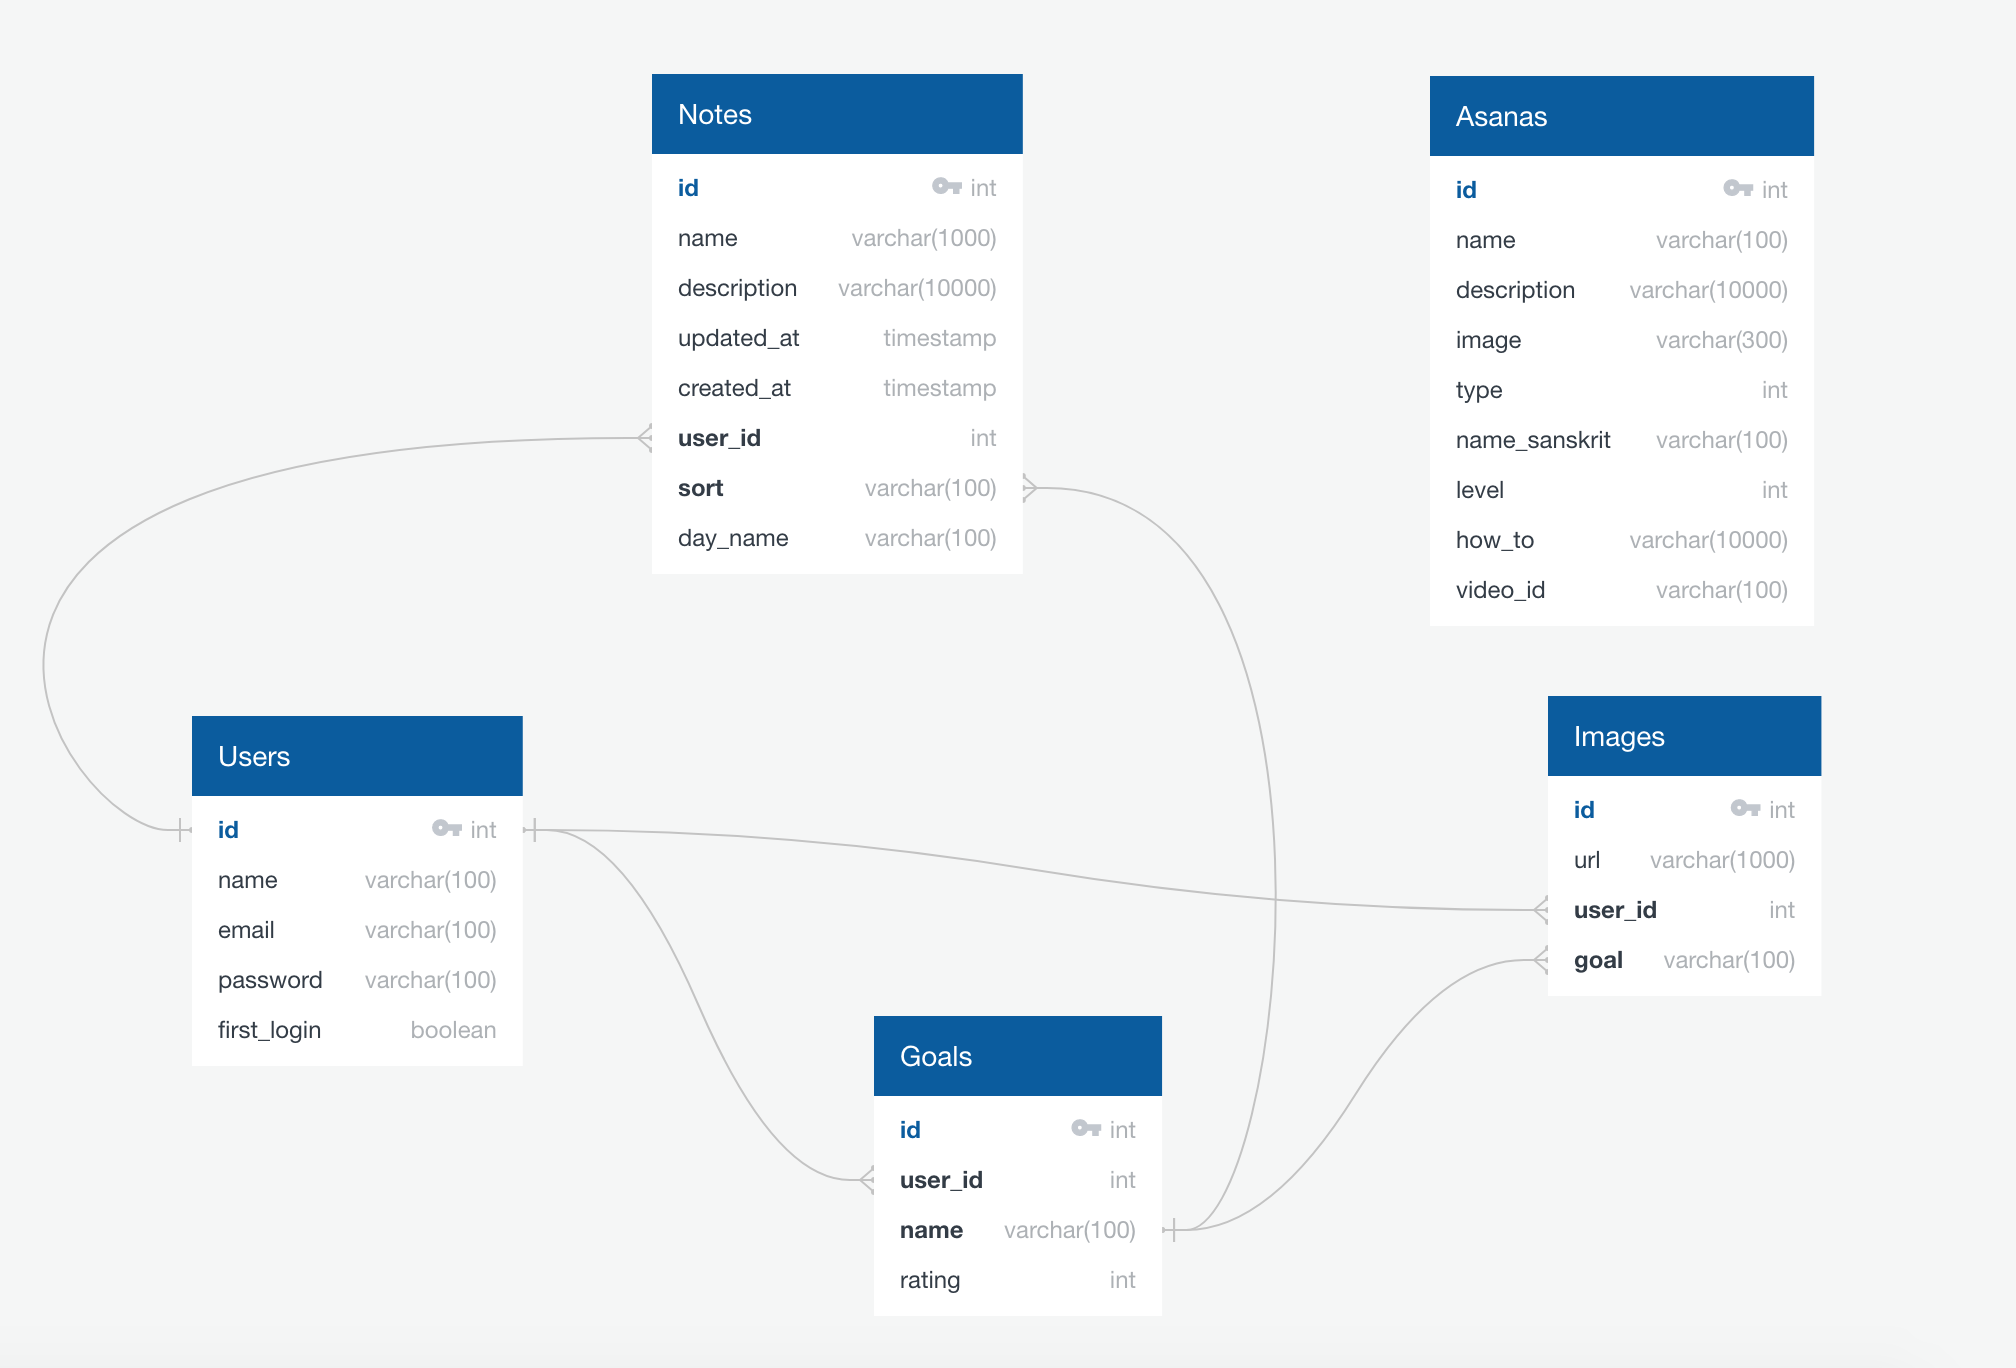
\includegraphics[scale=0.38]{diagram.png}
\end{center}
\caption{Fizični model podatkovne baze.}
\label{baza}
\end{figure}

\section{Logični nivo}
Logični nivo predstavlja REST API. Za njegov ravoj je bilo uporabljeno ogrodje Express.

\begin{figure}[htbp]
\begin{center}
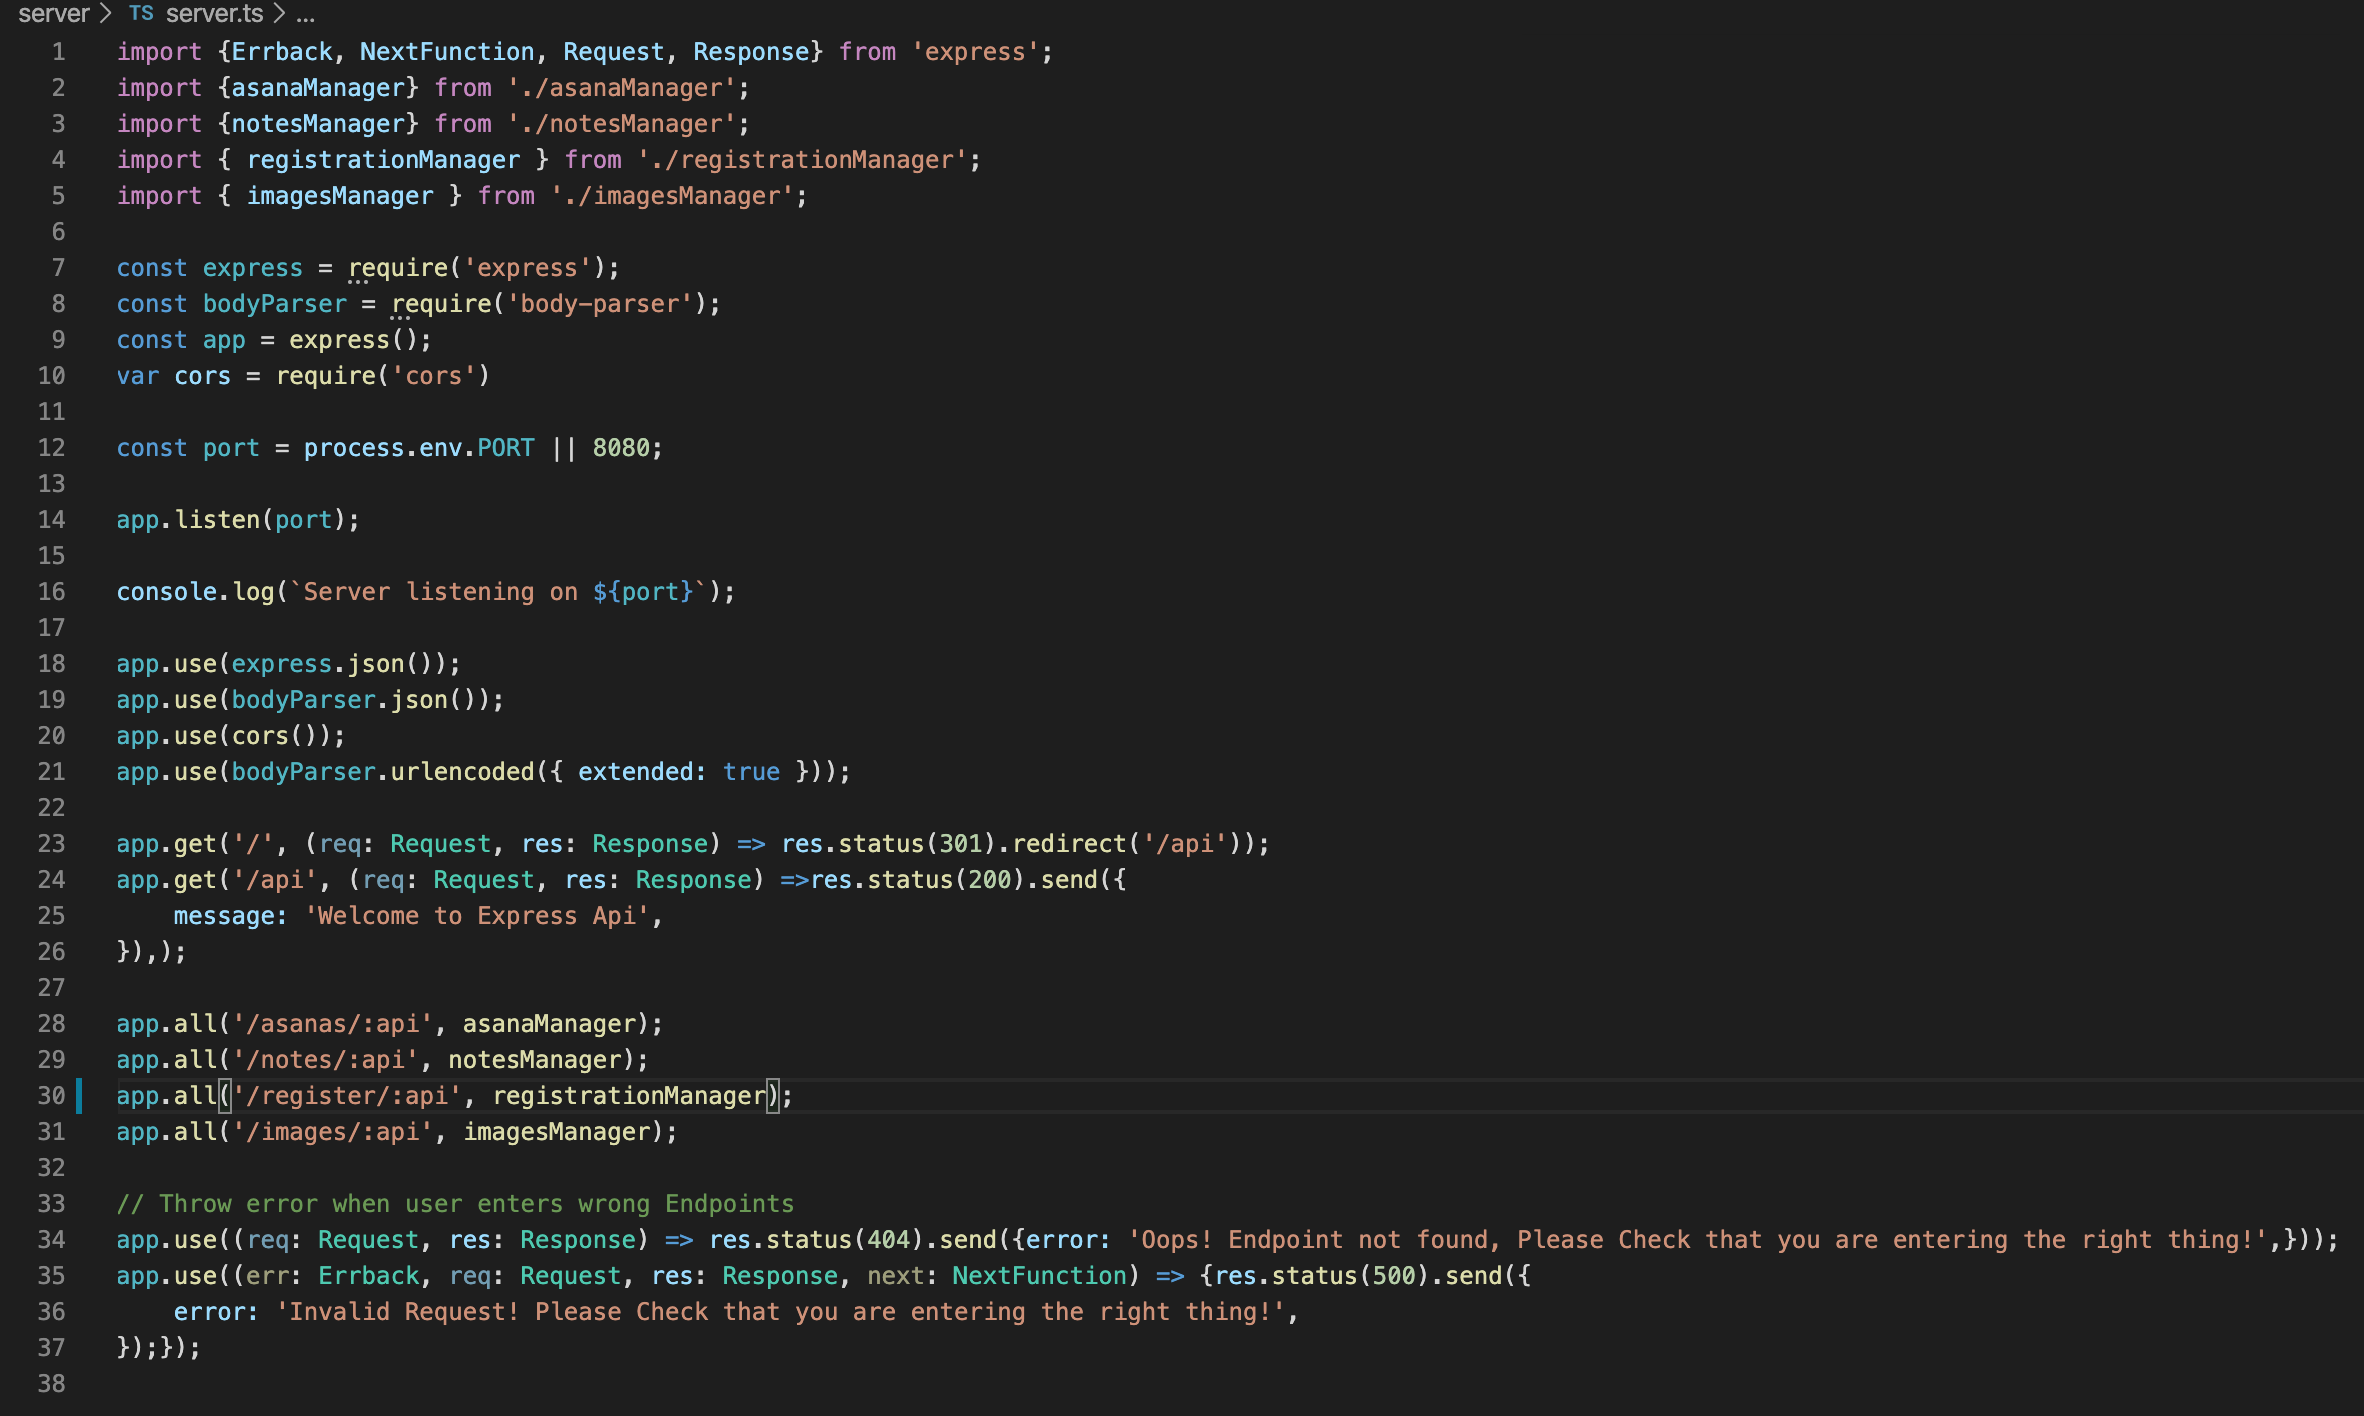
\includegraphics[scale=0.33]{server.jpg} 
\end{center}
\caption{Koda za vzpostavitev REST API serverja.}
\label{server}
\end{figure}

API je v aplikaciji posrednik med podatkovno bazo in uporabniki aplikacije. Sprejema zahtevke s strani uporabe aplikacije in izvaja ustrezne operacije na podatkovni bazi. Uporabljeni so bili naslednji zahtevki HTTP za različne namene:

 \begin{itemize}
  \item \textbf{GET}: za pridobivanje podatkov o asanah, zapiske, slike in ostale vnose v podatkovni bazi
  \item \textbf{POST}: za dodajanje različnih vnosov v podatkovno bazo, kot je dodajanje slik ter zapiskov
  \item \textbf{DELETE}: za brisanje vnosov v podatkovni bazi
\end{itemize}

\section{Uporabniški nivo}
Uporabniški nivo predstavlja Android mobilna aplikacija. Za njen razvoj je bilo uporabljeno ogrodje Expo z React Native-om. Aplikacija s pošiljanjem zahtevkov HTTP komunicira z APIjem in od njega prejema odgovore, nato pa ustrezno posodobi uporabniški vmesnik.
Izdelava same mobilne aplikacije se je začela z izdelavo prototipa uporabniškega vmesnika mobilne aplikacije, saj je izdelava dobrega uporabniškega vmesnika pomemben sestavni del oblikovanja uporabniške izkušnje. Vmesnik je narejen na bolj pregleden način, da je tako bolj enostaven za uporabo. Prav s tem namenom so v aplikacijo dodane tudi številne slike in videoposnetki.
Prototip je bil izdelan s pomočjo spletne platforme za izdelavo prototipov Proto.io, (Slika~\ref{protoio}). Izdelani so bili nekateri ključni zasloni aplikacije, glavne funkcionalnosti aplikacije, povezave med njimi, oblikovano glavno ozadje aplikacije na začetnem prijavnem zaslonu ter zaslonu za registracijo in oblikovan glavni meni aplikacije.

\begin{figure}[ht]
\begin{center}
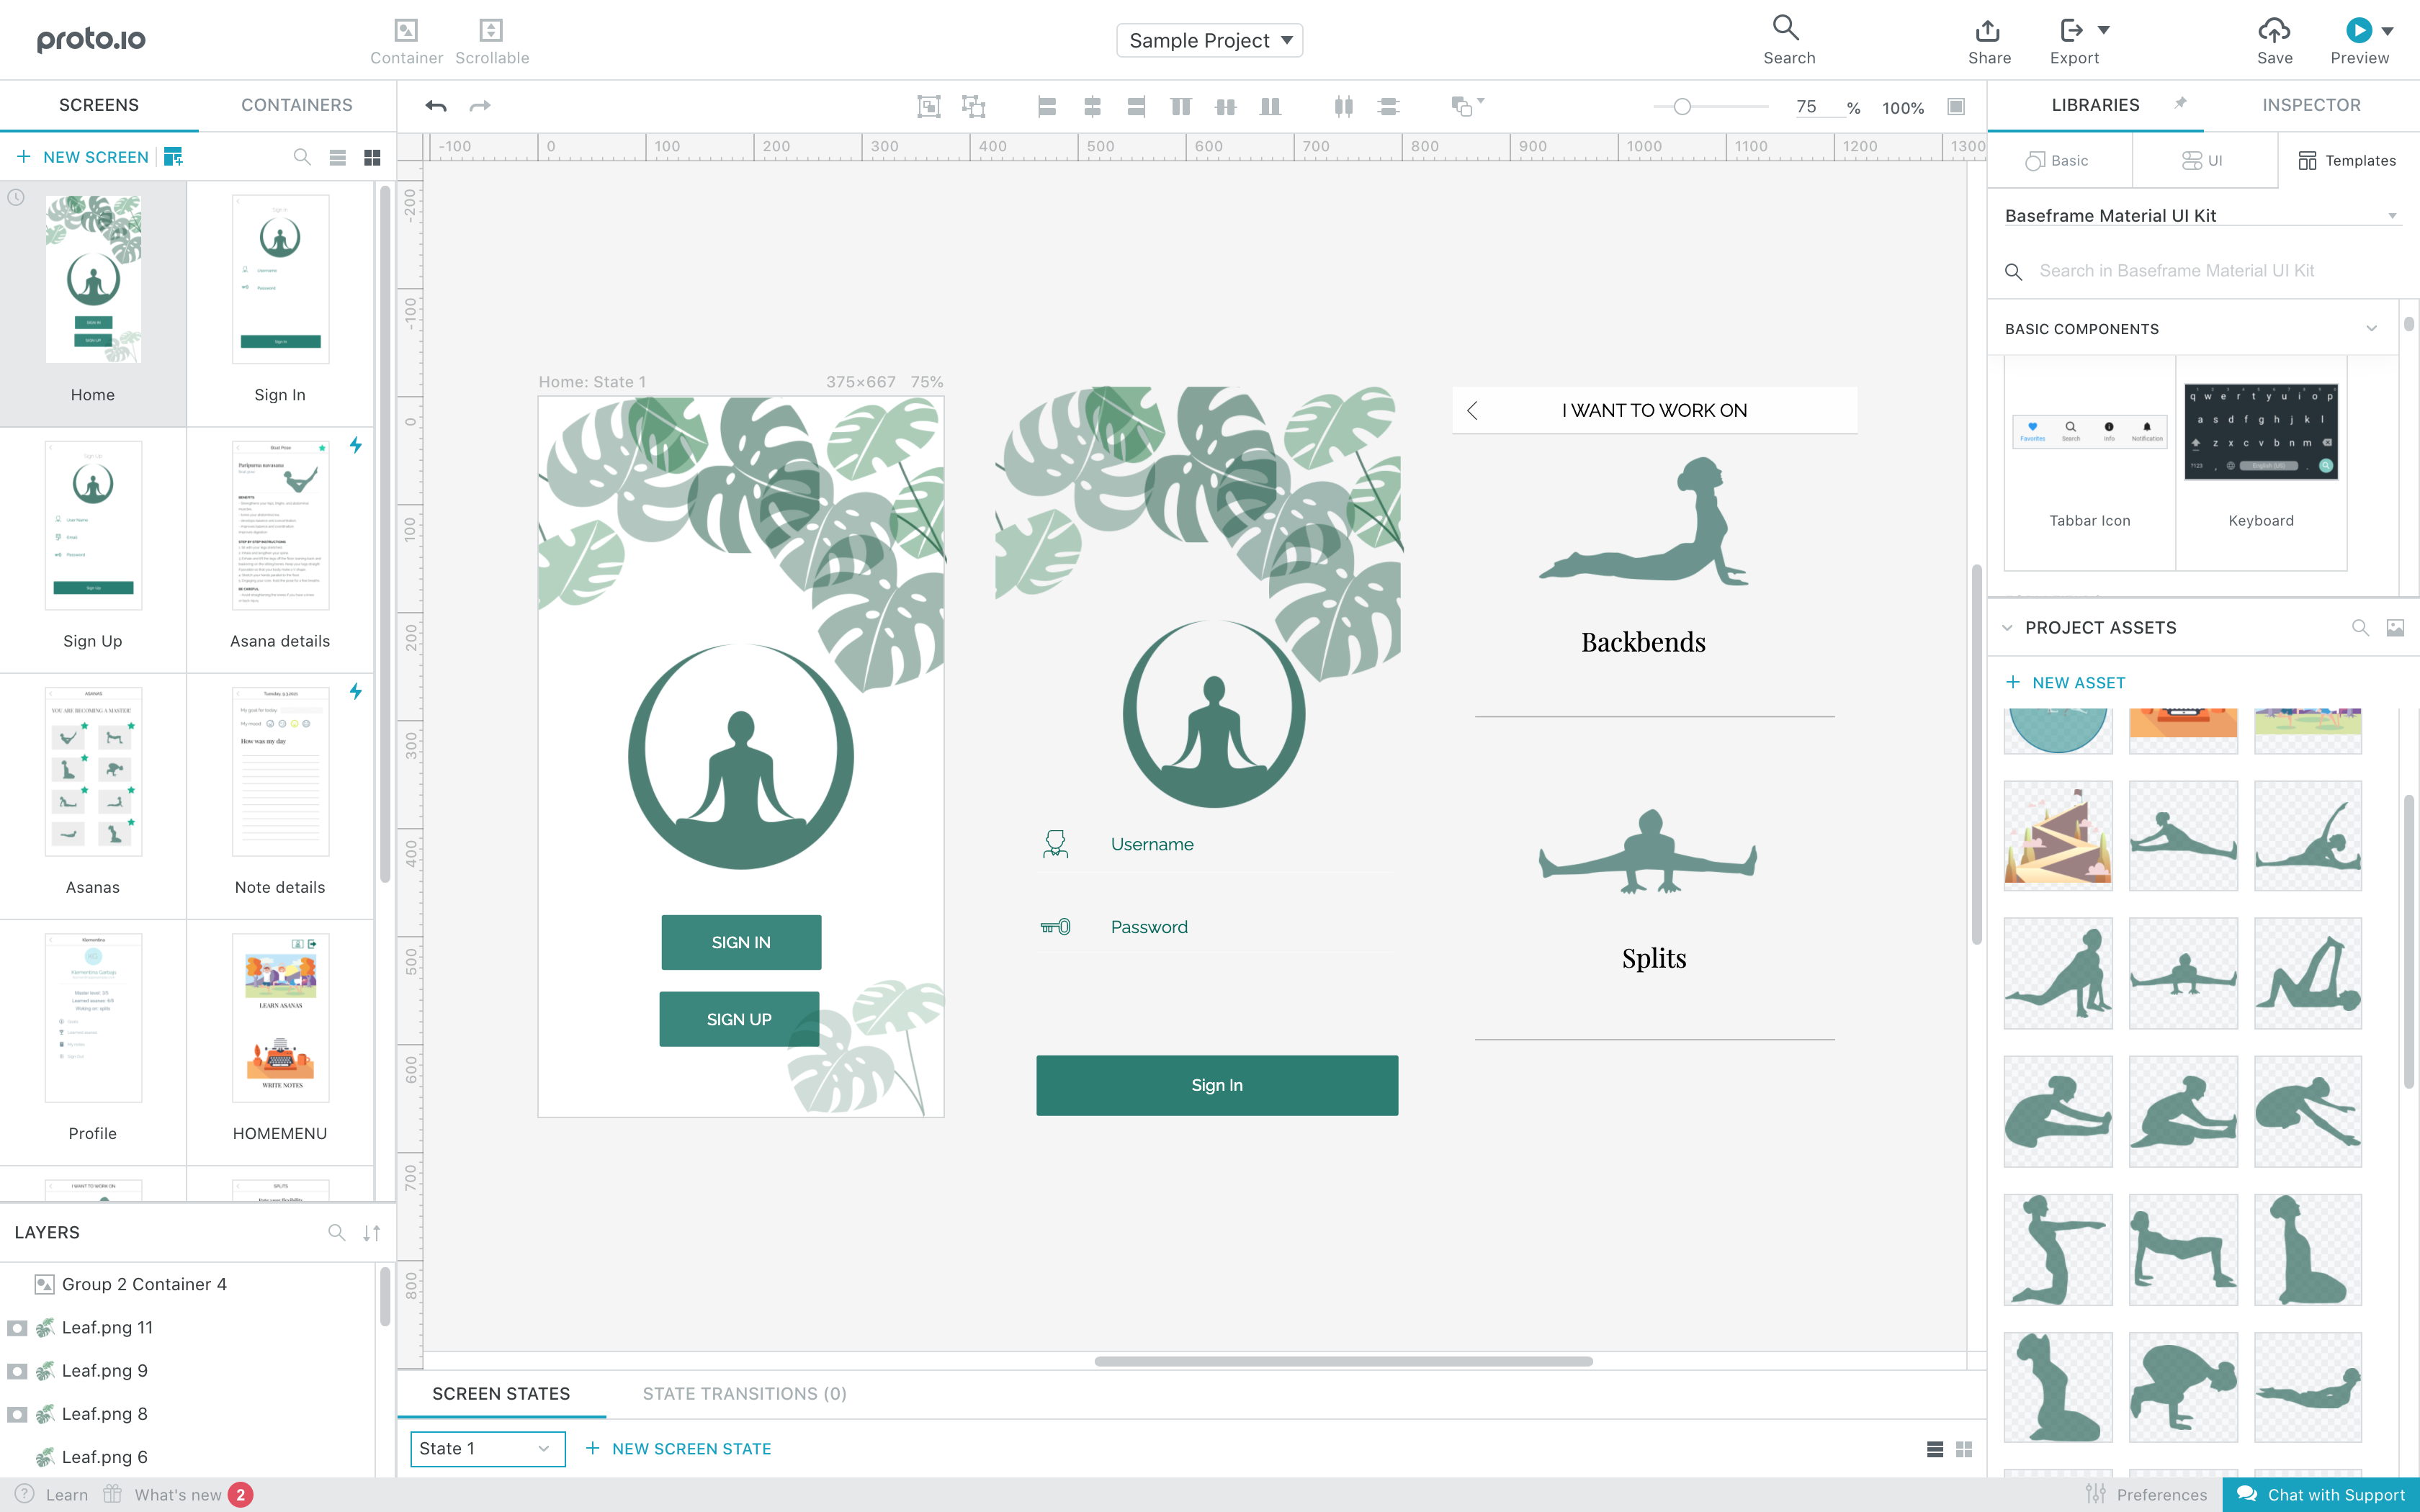
\includegraphics[scale=.23]{protoio.png}
\end{center}
\caption{Spletna platforma za ustvarjanje prototipov, Protoio.}
\label{protoio}
\end{figure}

Izdelavi prototipa je sledila raziskava tehnologij in primernih orodij za sam razvoj mobilne aplikacije, pri čemer je bila v ospredju primerjava različnih orodij za izdelavo mobilne aplikacije. Primerjana sta bila integrirano razvojno okolje (angl. integrated development environment, IDE) Android Studio za razvoj aplikacij za operacijski sistem Android, ter razvojno okolje Expo, ki z uporabo React Native platforme in orodij, omogoča razvoj tako spletnih, kot mobilnih aplikacij na operacijskem sistemu Android in iOS. Zaradi možnosti razvoja na obeh operacijskih sistemih ter predhodnih izkušenj, je bilo nazadnje, za razvoj mobilne aplikacije, izbrano razvojno okolje Expo.

Po začetnem načrtovanju prototipa aplikacije je sledilo še zbiranje podatkov o jogi in položajih v jogi. 


\chapter{Predstavitev aplikacije}
\label{ch3}
\section{Funkcionalnosti in delovanje aplikacije}
Za zagon aplikacije je potrebno najprej vzpostaviti povezavo s strežnikom z ukazom "npm run server", nato pa se z ukazom "npm web build" zažene testno okolje Expo Developer Tools. V testnem okolju se nahaja možnost testiranja mobilne aplikacije na Android emulatorju, lahko pa se aplikacija testira preko mobilne naprave s skeniranjem QR kode, (Slika~\ref{reactDevTools}).
  
\begin{figure}[ht]
\centering
  \begin{minipage}[b]{1\textwidth}
    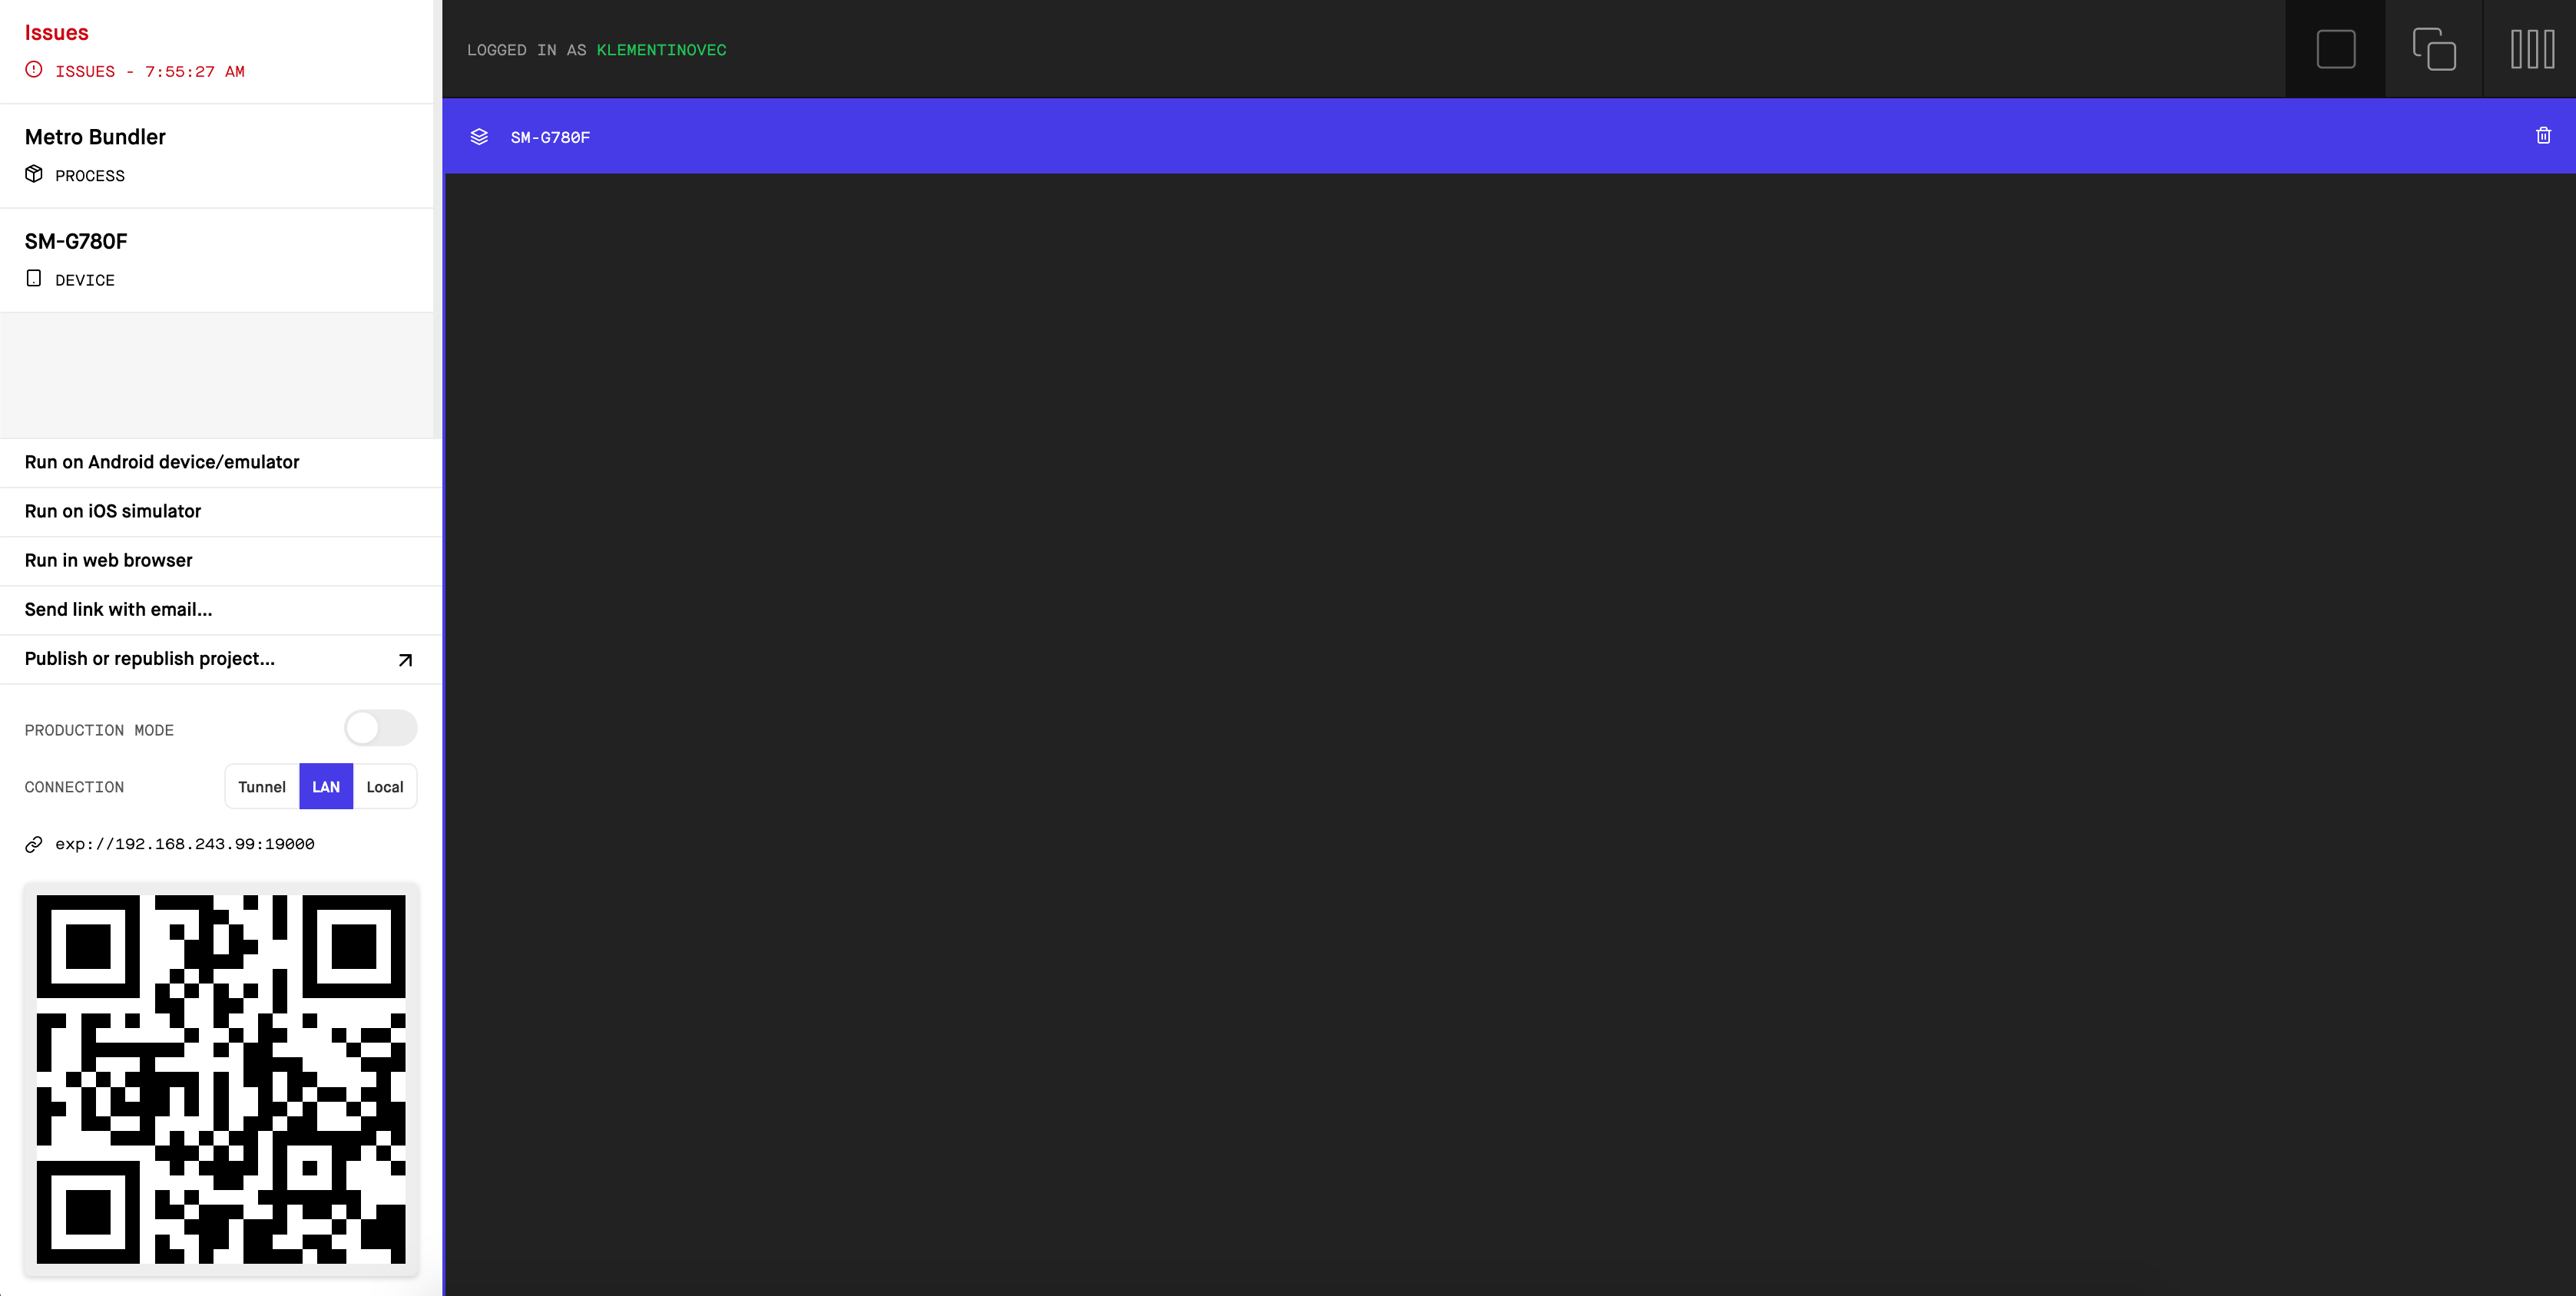
\includegraphics[width=\textwidth]{expodeveloper.png}\centering
  \end{minipage}
    \caption{Expo Developer Tools testno okolje na spletnem vmesniku.}
    \label{reactDevTools}
\end{figure}

Ob zagonu mobilne aplikacije je uporabnik najprej preusmerjen na stran za prijavo, (Slika~\ref{prijava}, levo). Uporabnik, ki že ima uporabniško ime in geslo, se lahko s klikom na Sign in enostavno prijavi v aplikacijo z že obstoječimi podatki. V kolikor uporabnik še ni registriran, mora najprej opraviti registracijo, s klikom na gumb Sign up, kar ga preusmeri na stran za registracijo, (Slika~\ref{prijava}, desno). Za uspešno registracijo mora vnesti svoje ime, svoj elektronski naslov in geslo, ki ga bo uporabljal za prijavo. Ob registraciji uporabnika se v podatkovno bazo shrani nov uporabnik z vnesenimi podatki in sproži se prijava uporabnika.

\begin{figure}[ht]
\centering
  \begin{minipage}[b]{0.43\textwidth}
    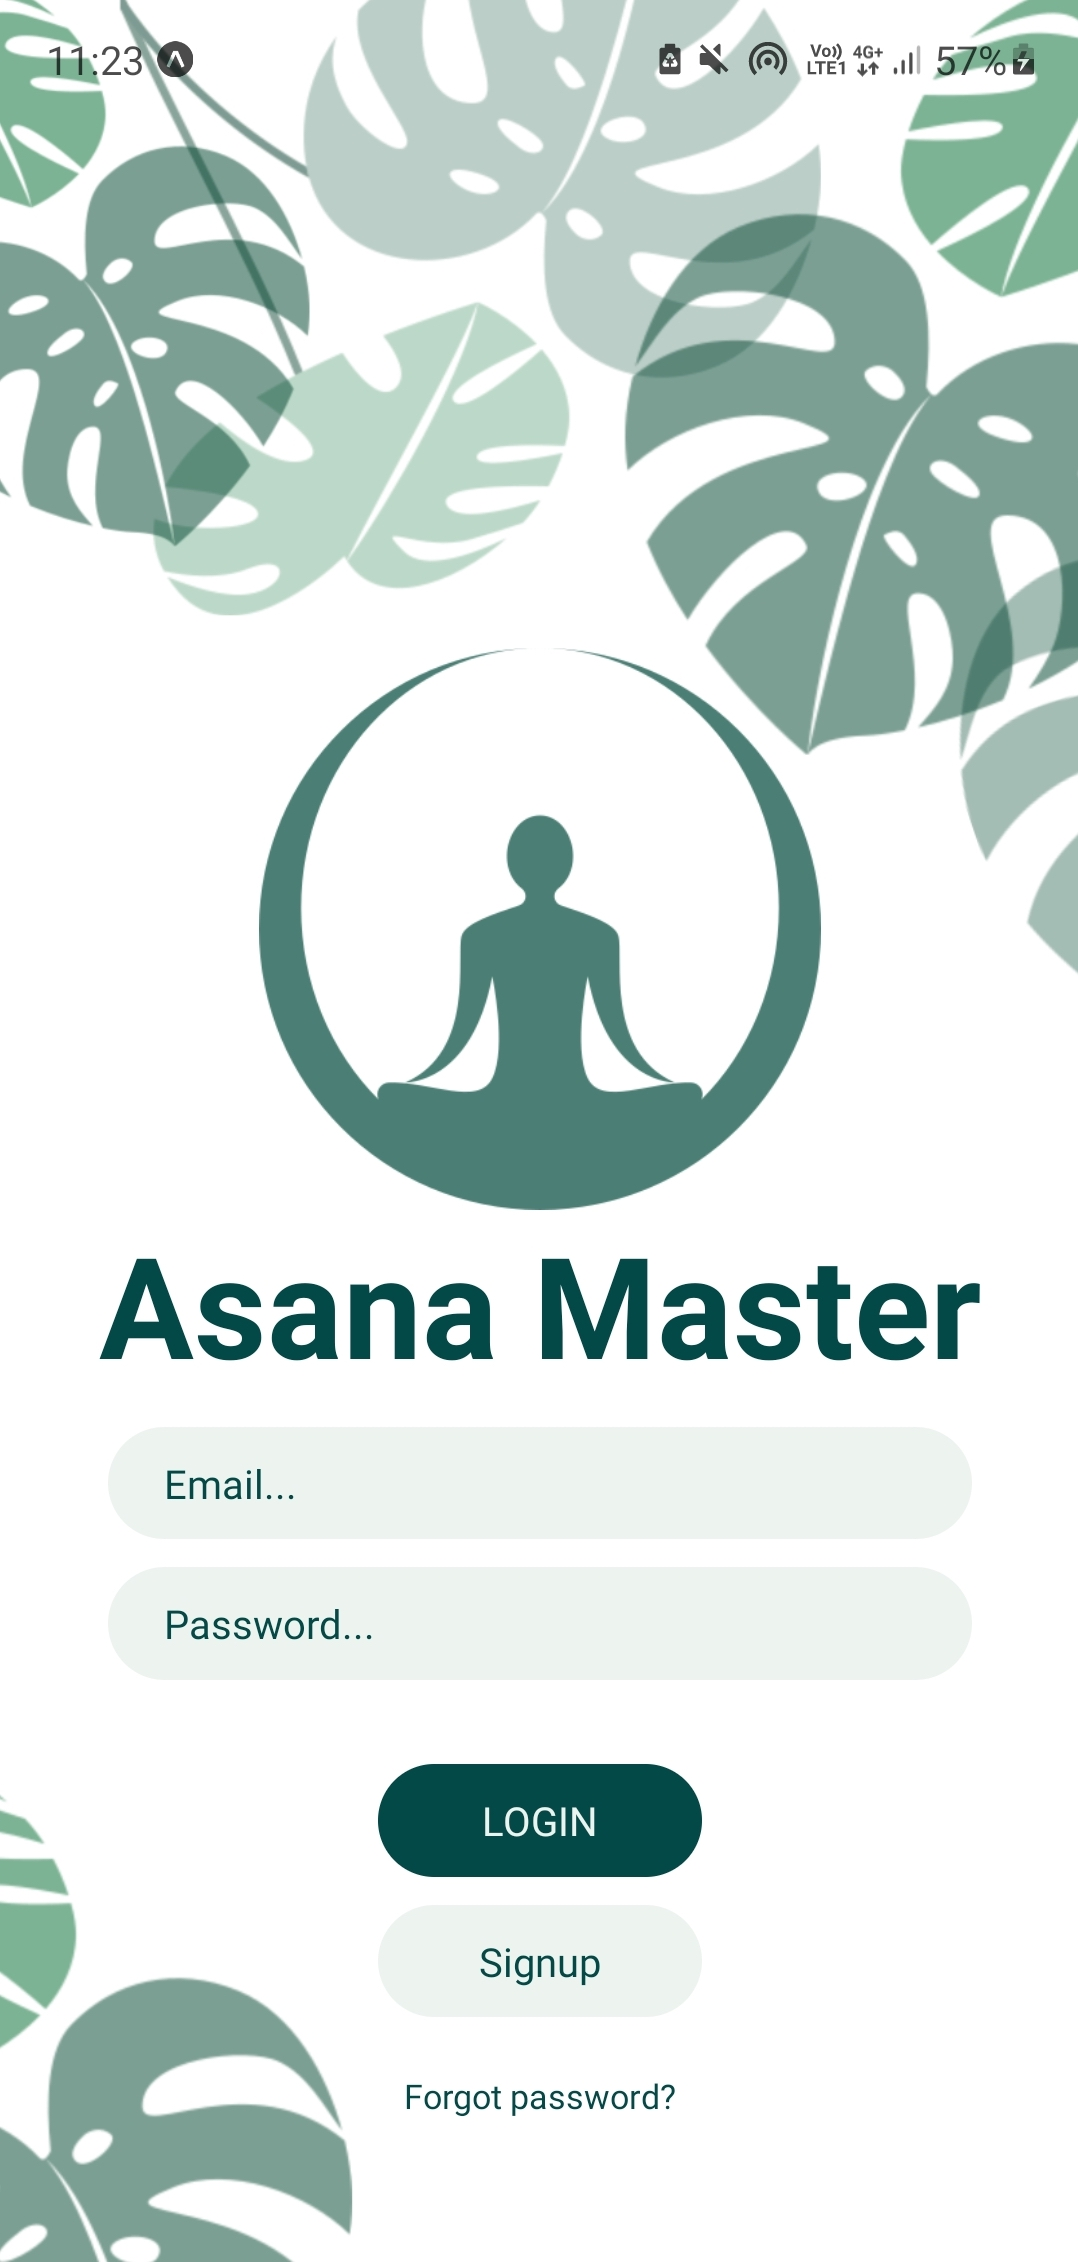
\includegraphics[width=\textwidth]{prijava.jpg}\centering
    \label{prijava}
  \end{minipage}
  \begin{minipage}[b]{0.43\textwidth}
    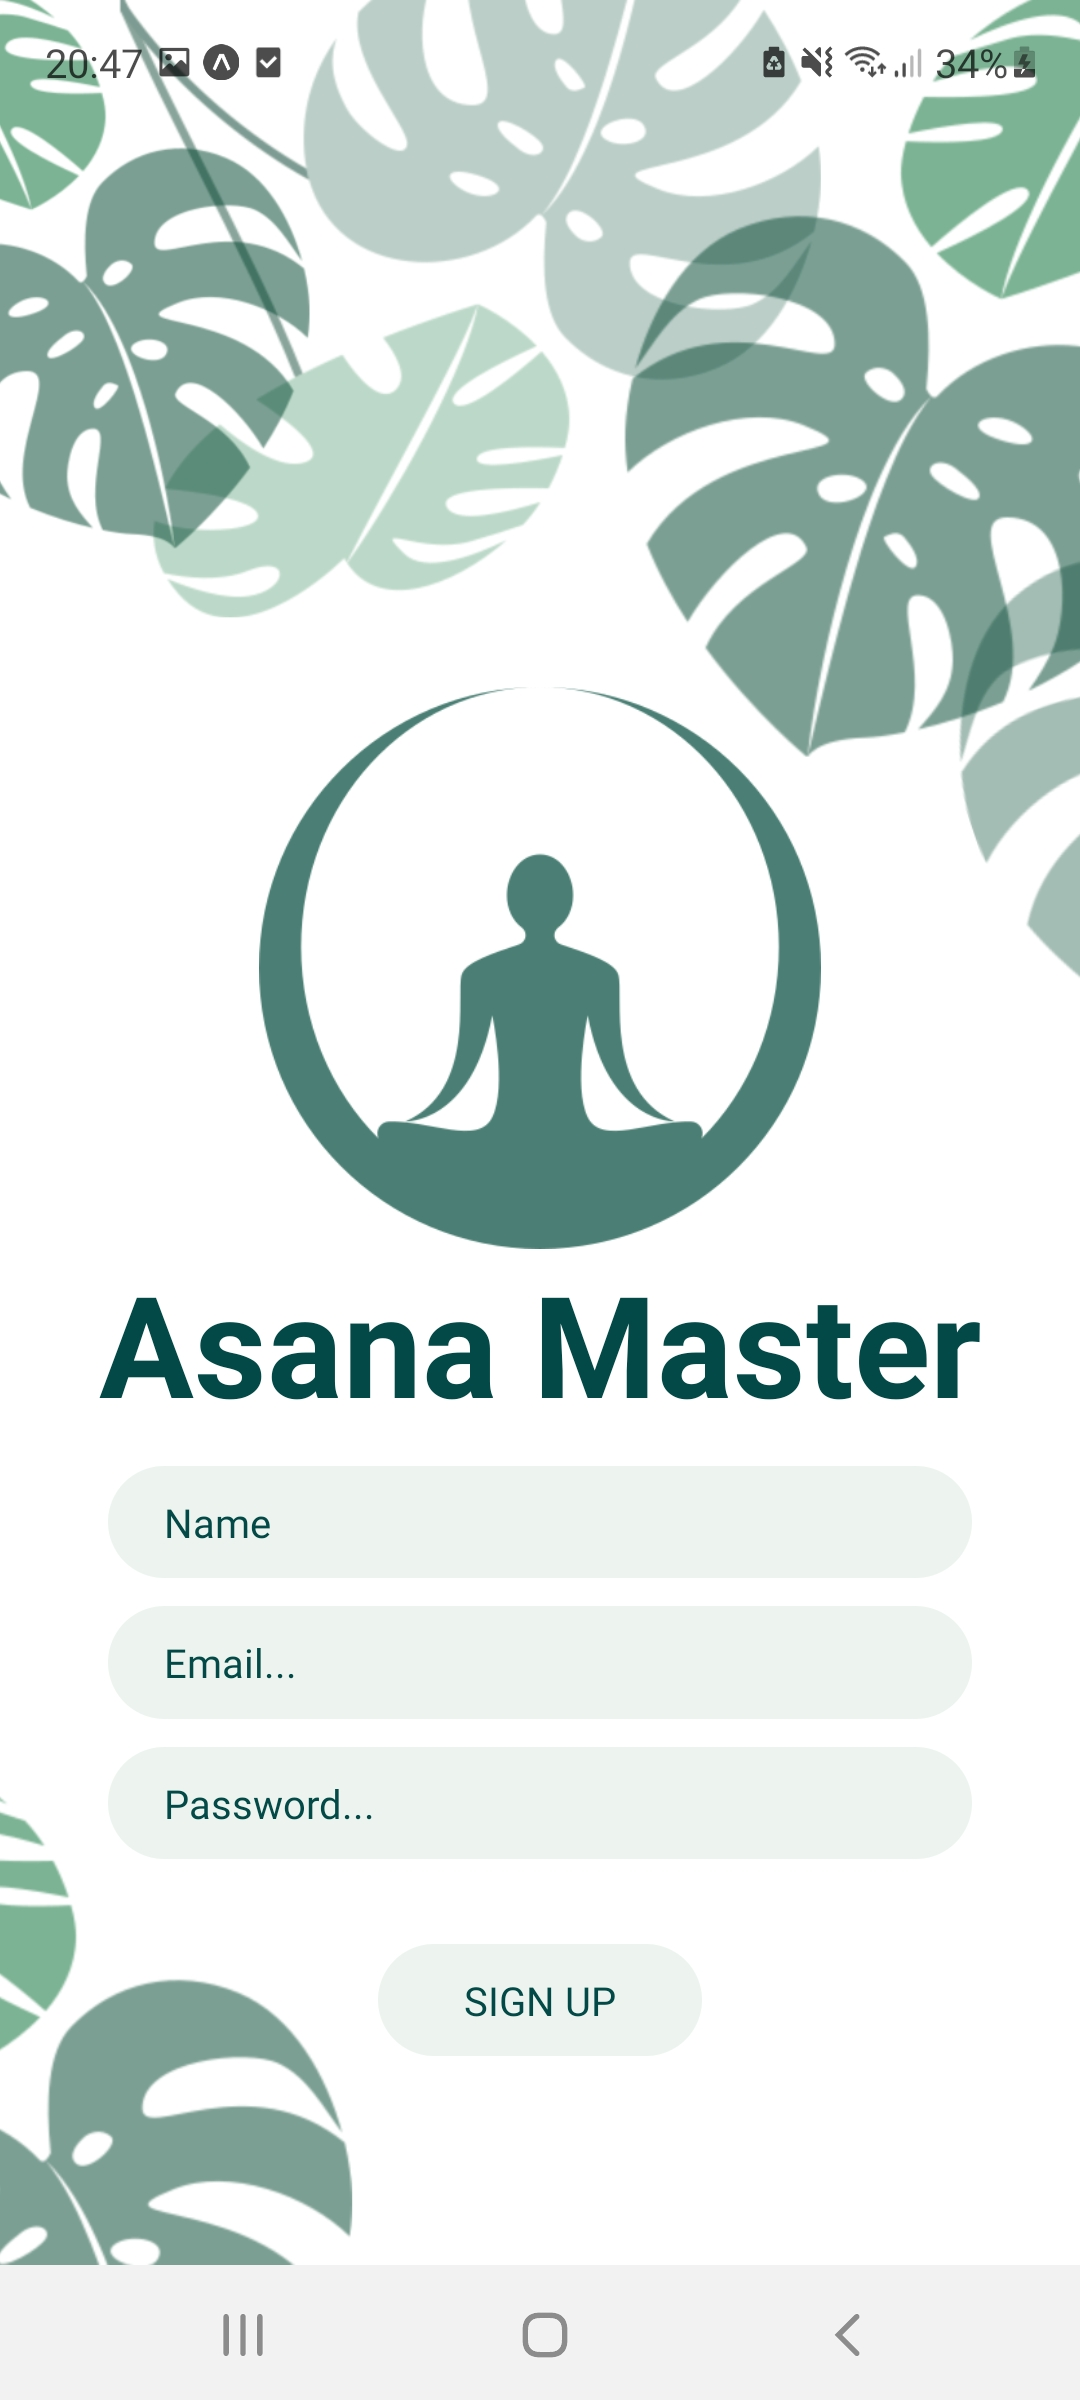
\includegraphics[width=\textwidth]{registracija.jpg}\centering
  \end{minipage}
    \caption{Obrazec za prijavo (levo) in registracijo (desno)}
\end{figure}

Ob prvi prijavi, uporabnika ob vstopu v aplikacijo pozdravi kratek uvod v aplikacijo, (Slika~\ref{pozdrav}). Pozdrav je predstavljen na dveh straneh, med katerima se lahko uporabnik poljubno premika. Na prvi strani se uporabnik seznani s pojmom joga in na drugi strani s kratkim opisom aplikacije.

\begin{figure}[ht]
\centering
  \begin{minipage}[b]{0.43\textwidth}
    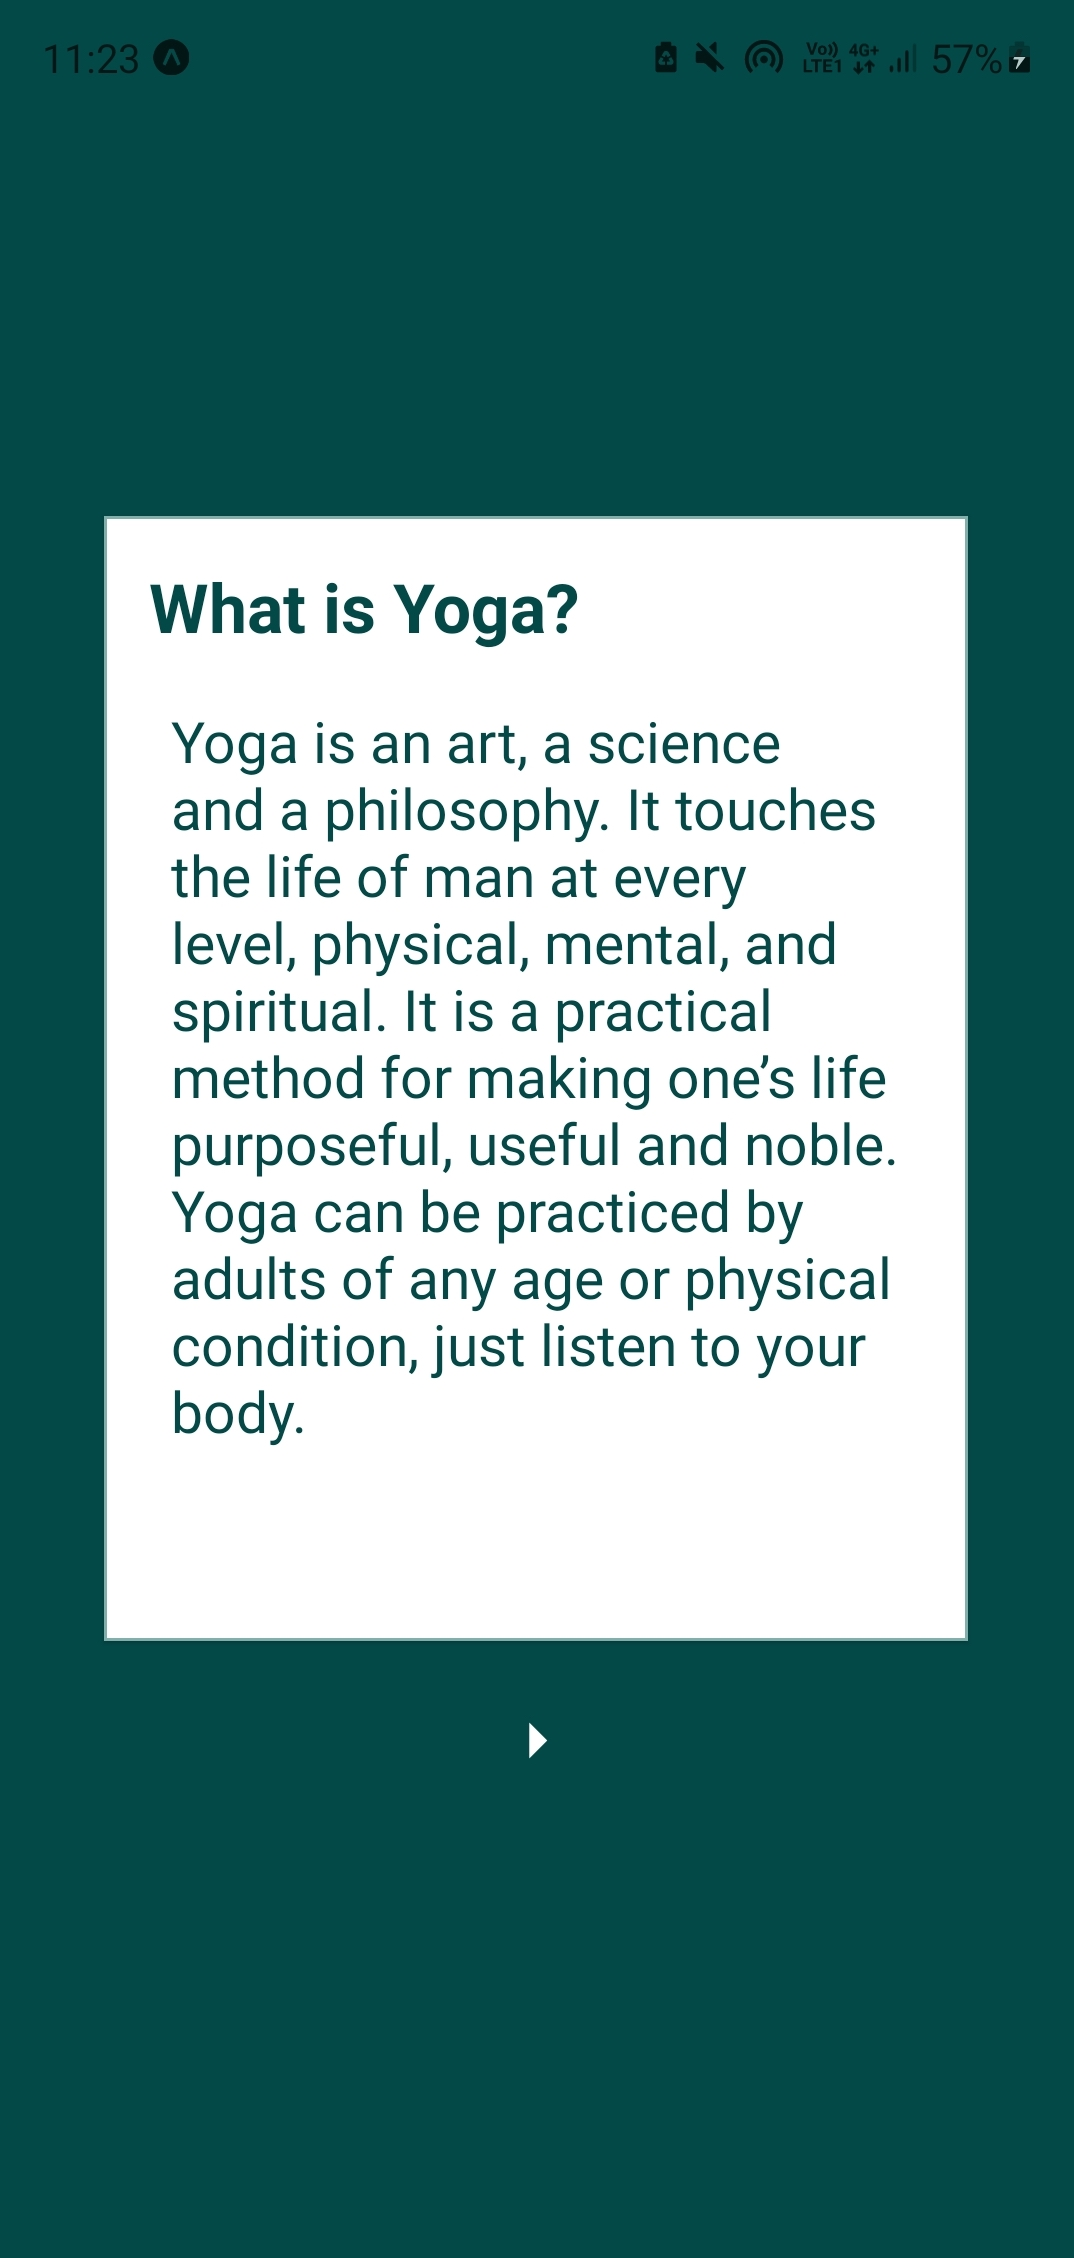
\includegraphics[width=\textwidth]{pozdrav1.jpg}\centering
    \label{pozdrav}
  \end{minipage}
  \begin{minipage}[b]{0.43\textwidth}
    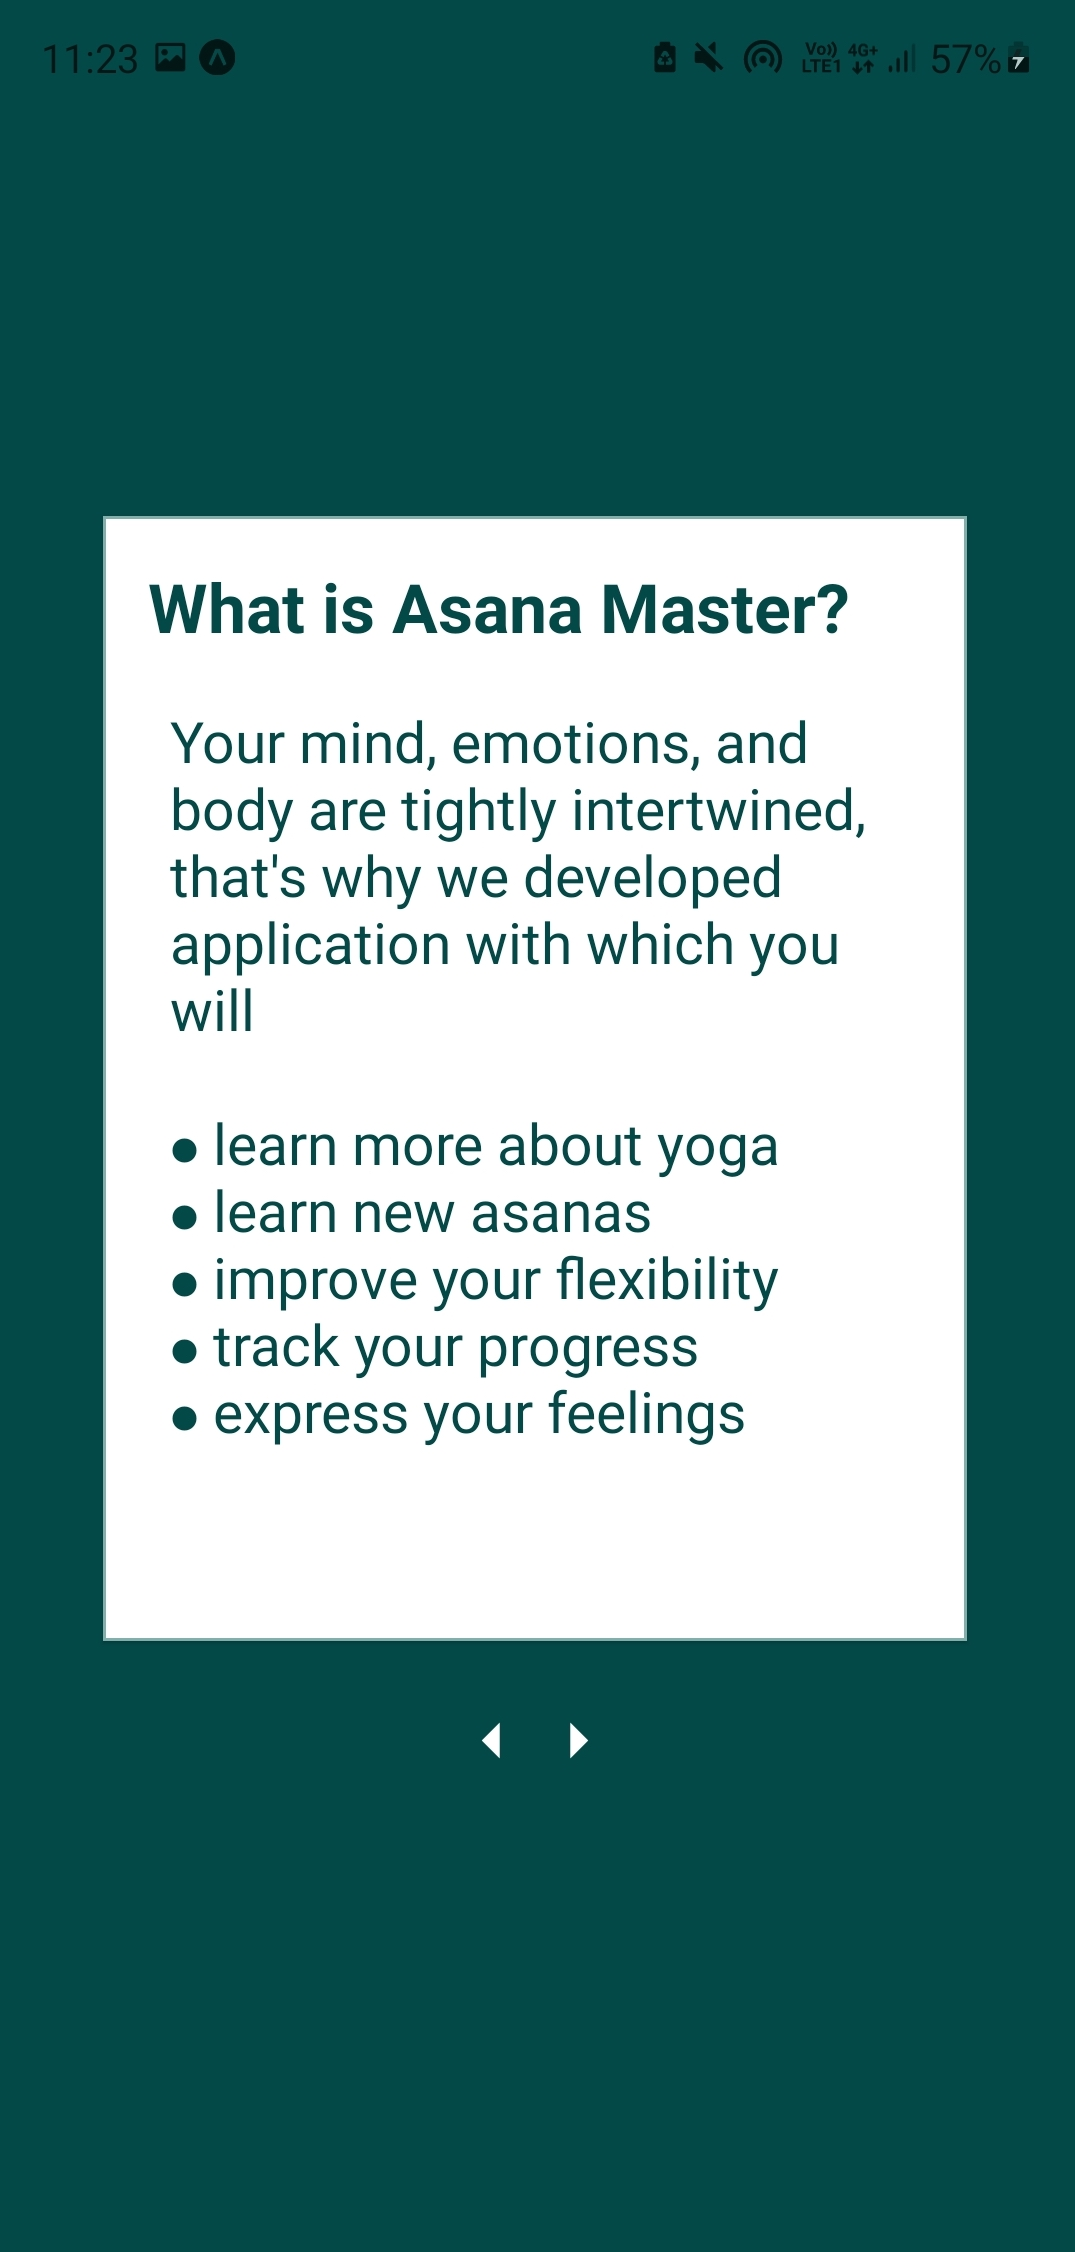
\includegraphics[width=\textwidth]{pozdrav2.jpg}\centering
  \end{minipage}
    \caption{Prva in druga stran začetnega pozdrava, ob prvi prijavi uporabnika.  }
\end{figure}

Po začetnem uvodu v aplikacijo ali po n-ti prijavi v aplikacijo, je uporabnik nato preusmerjen v glavni meni, (Slika~\ref{menu}). V glavnem meniju se uporabnik lahko premika levo in desno in izbira med tremi podmeniji. Podmeniji, ki so na voljo, so: "Asanas", "Goals" in "Notes". V glavnem meniju se zgoraj desno nahaja tudi gumb za odjavo.

\begin{figure}[!ht]
\centering
  \begin{minipage}[b]{0.325\textwidth}
    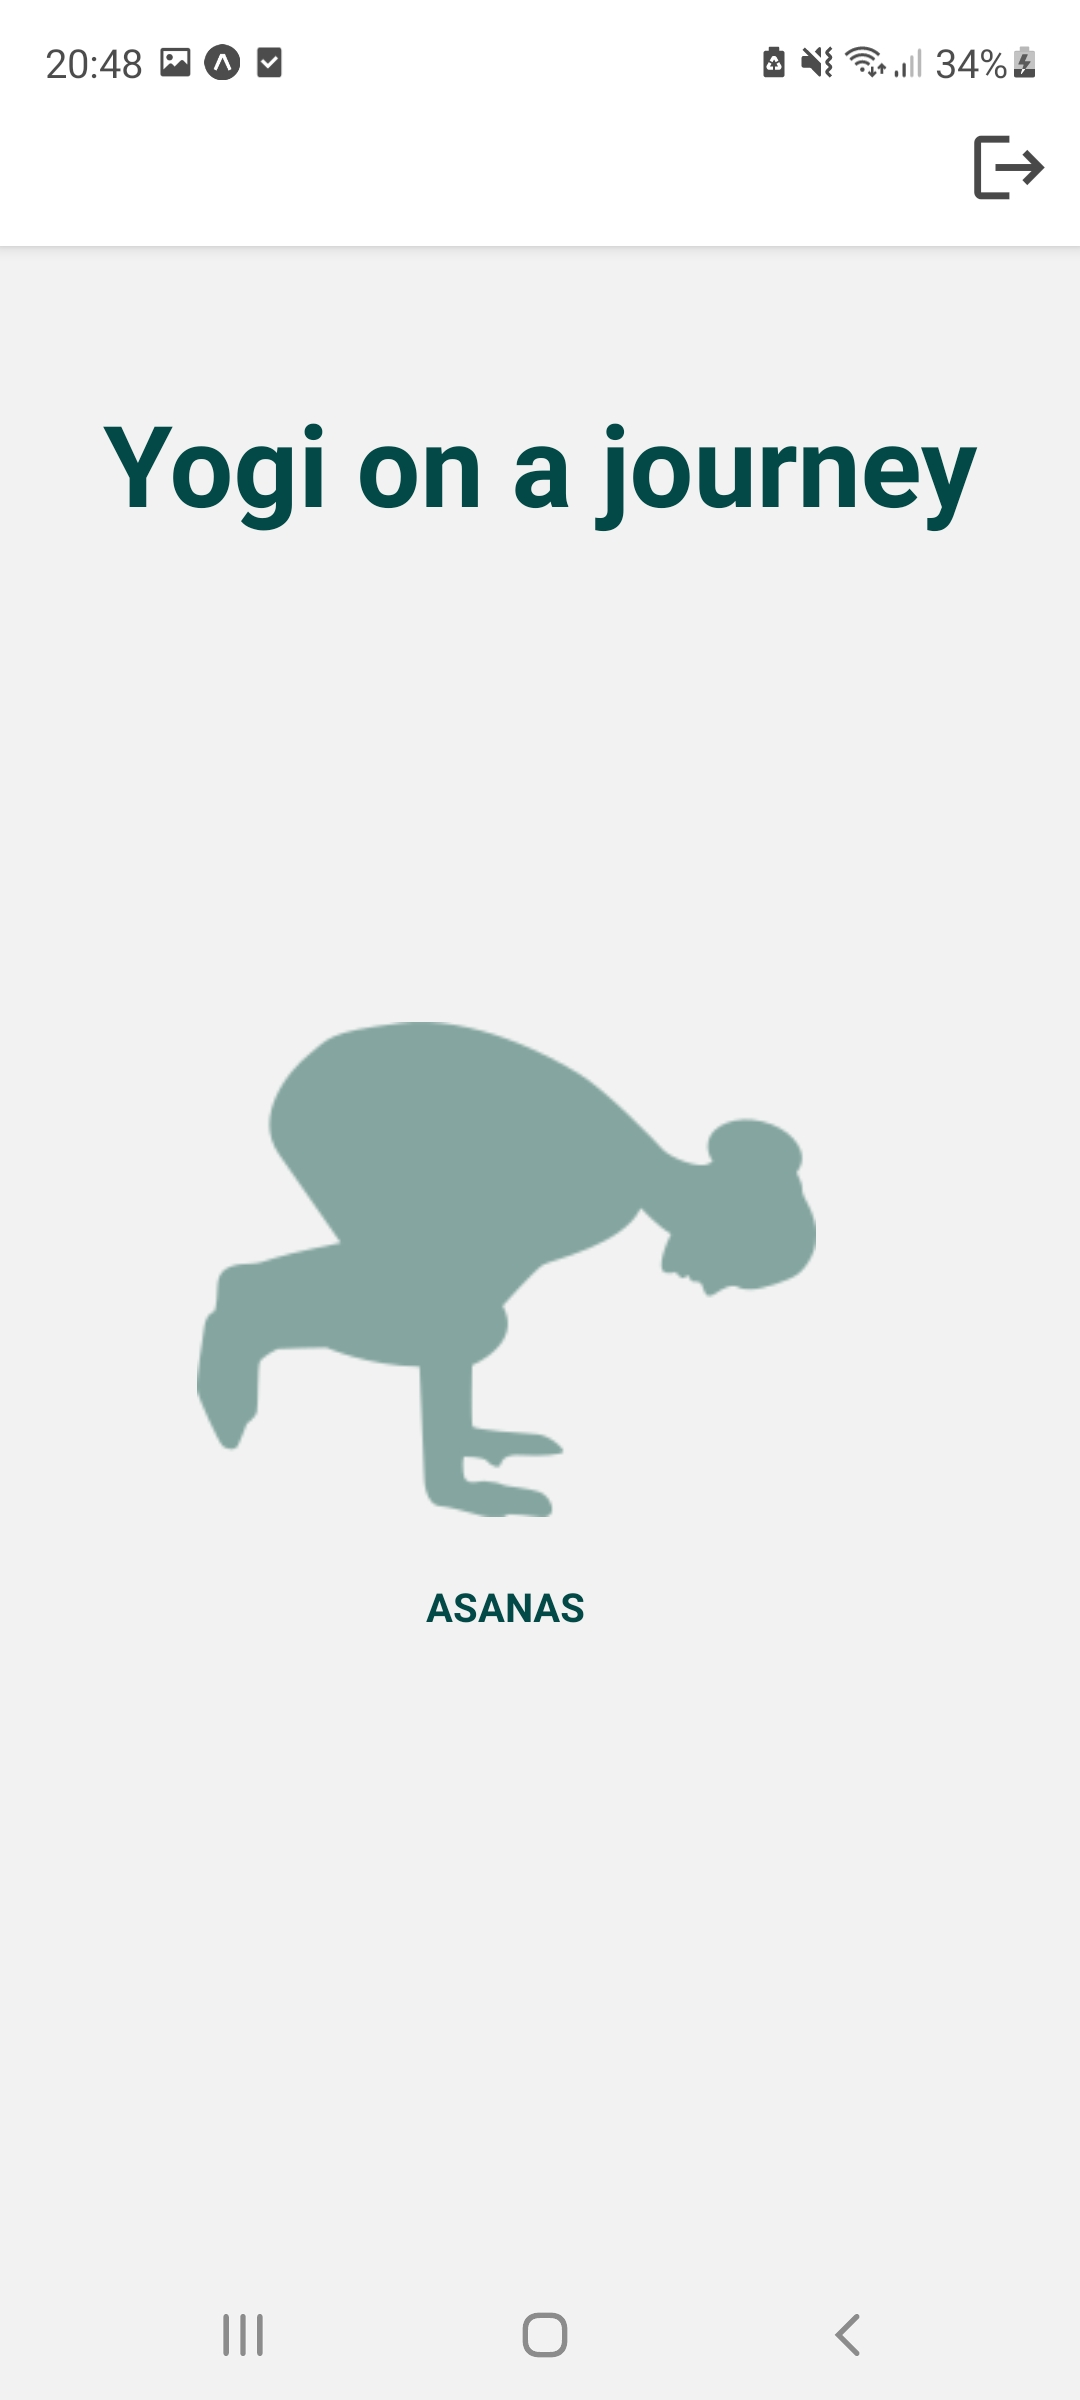
\includegraphics[width=\textwidth]{menu1.jpg}\centering
    \label{menu}
  \end{minipage}
  \begin{minipage}[b]{0.325\textwidth}
    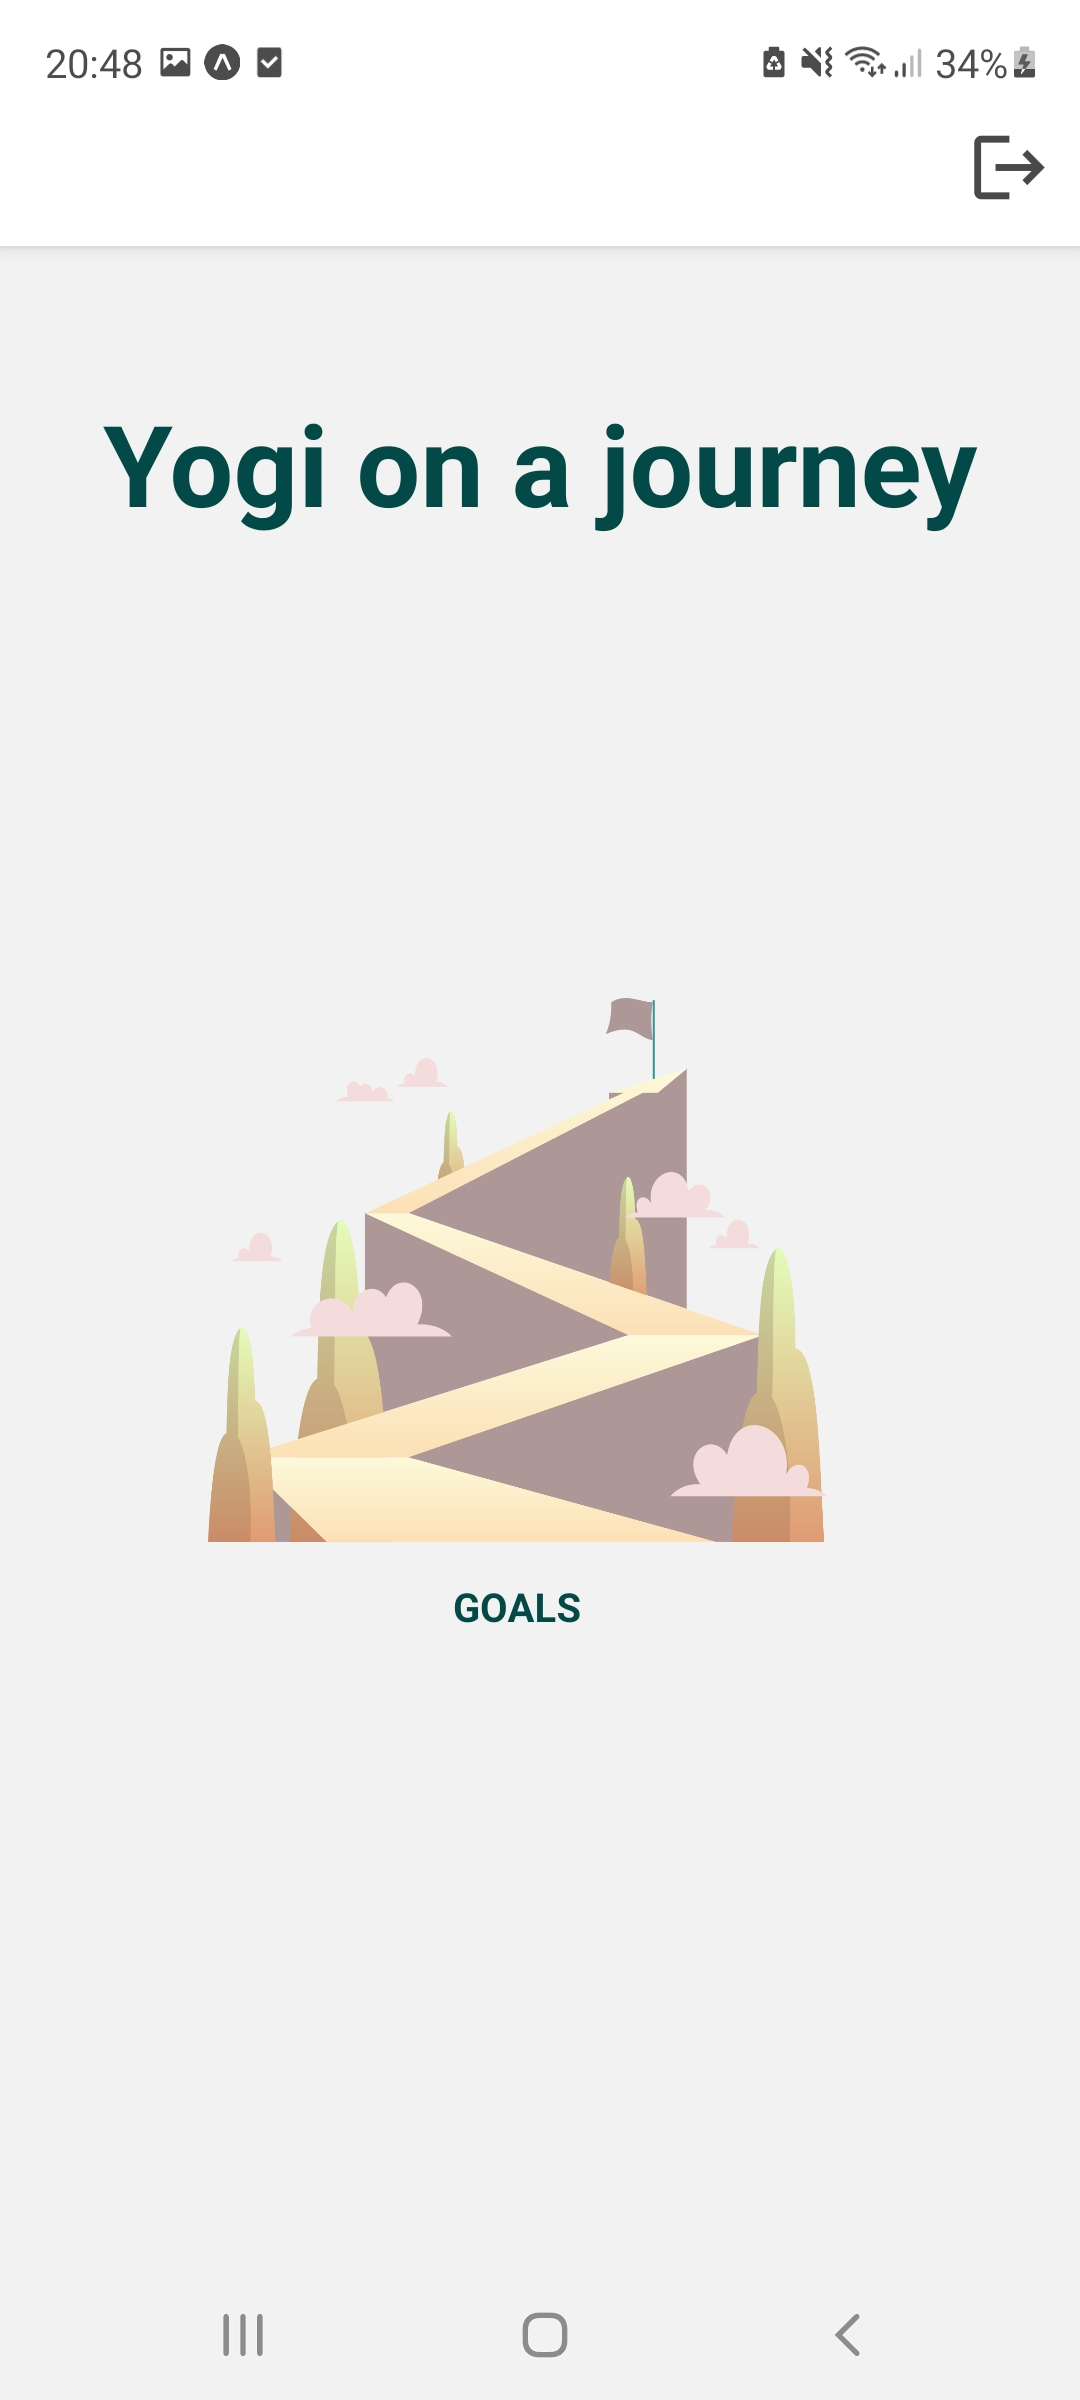
\includegraphics[width=\textwidth]{menu2.jpg}\centering
  \end{minipage}
  \begin{minipage}[b]{0.325\textwidth}
    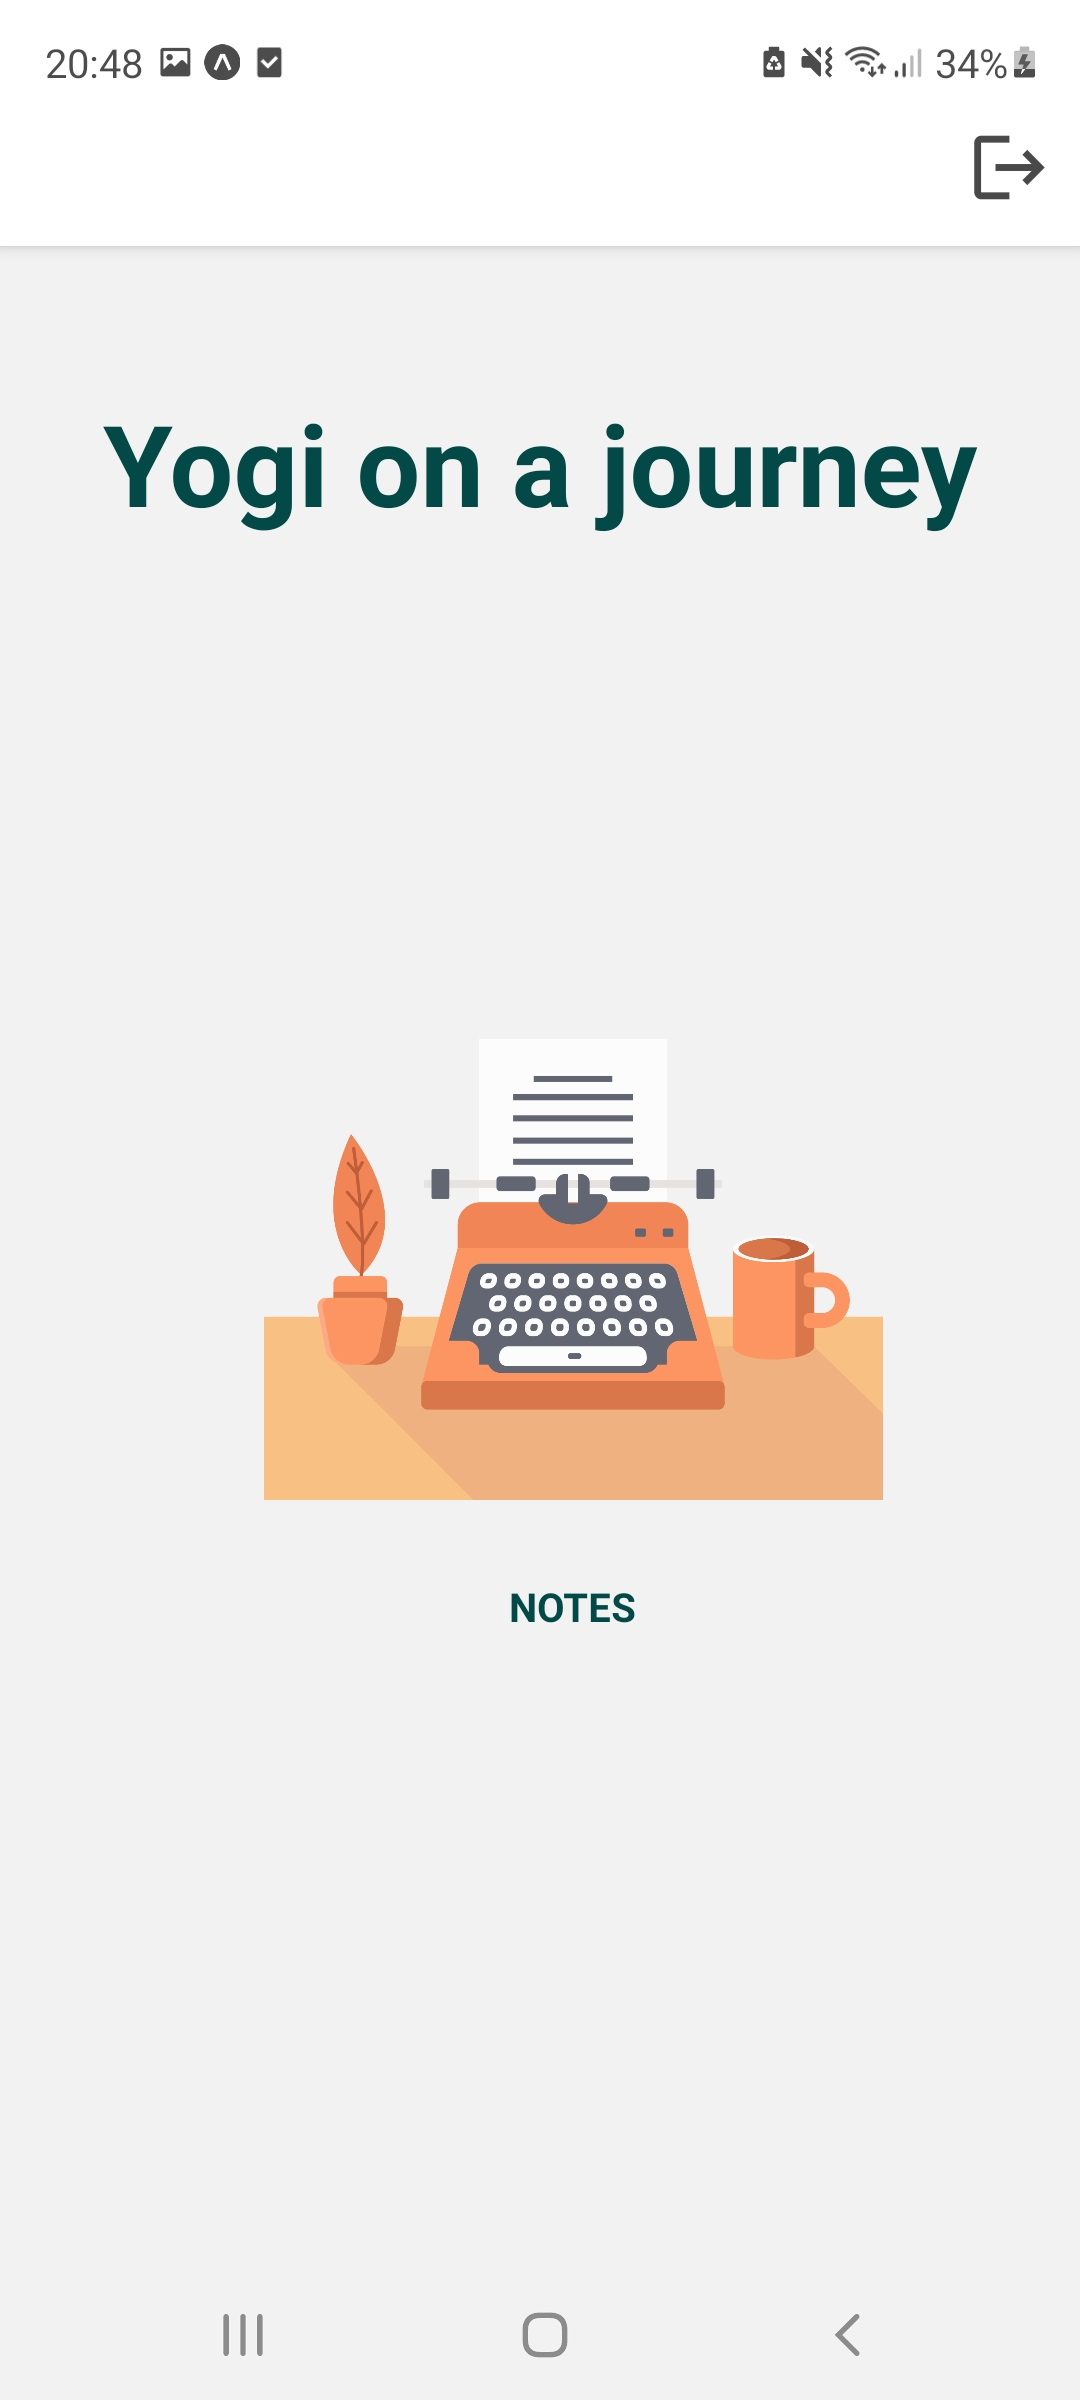
\includegraphics[width=\textwidth]{menu3.jpg}\centering
  \end{minipage}
    \caption{Glavni meni s tremi možnostmi izbire podmenija (\textit{Asanas}, \textit{Goals}, \textit{Notes}).}
\end{figure} 

Podmeni \textit{Asanas} je razdeljen na tri dodatne podmenije, ki določajo različne kategorije težavnosti položajev. Kategorije težavnosti so: \textit{Begginer}, \textit{Intermediate}, in \textit{Master}, (Slika~\ref{asana}). \\
S klikom na eno izmed naštetih težavnosti se uporabniku odpre dodaten podmeni, kjer se nahaja seznam z imeni in slikami položajev določene težavnosti. S klikom na enega izmed položajev, se odpre stran z angleškim imenom, sanskrit imenom, sliko, pozitivnimi učinki položaja, razdelek \textit{How to} z opisom izvedbe po korakih in videoposnetkom položaja za ogled same izvedbe, (Slika~\ref{asana2}). Uporabnik ima možnost ogleda videoposnetka položaja, s klikom na videoposnetek. Videoposnetek se predvaja neposredno v aplikaciji, kjer ima uporabnik tudi možnost povečave videa skozi celoten ekran mobilne naprave, s klikom na naslov posnetka pa si ga uporabnik lahko ogleda tudi izven aplikacije na platformi Youtube.\\

\begin{figure}[!htbp]
\centering
\begin{minipage}[b]{0.32\textwidth}
    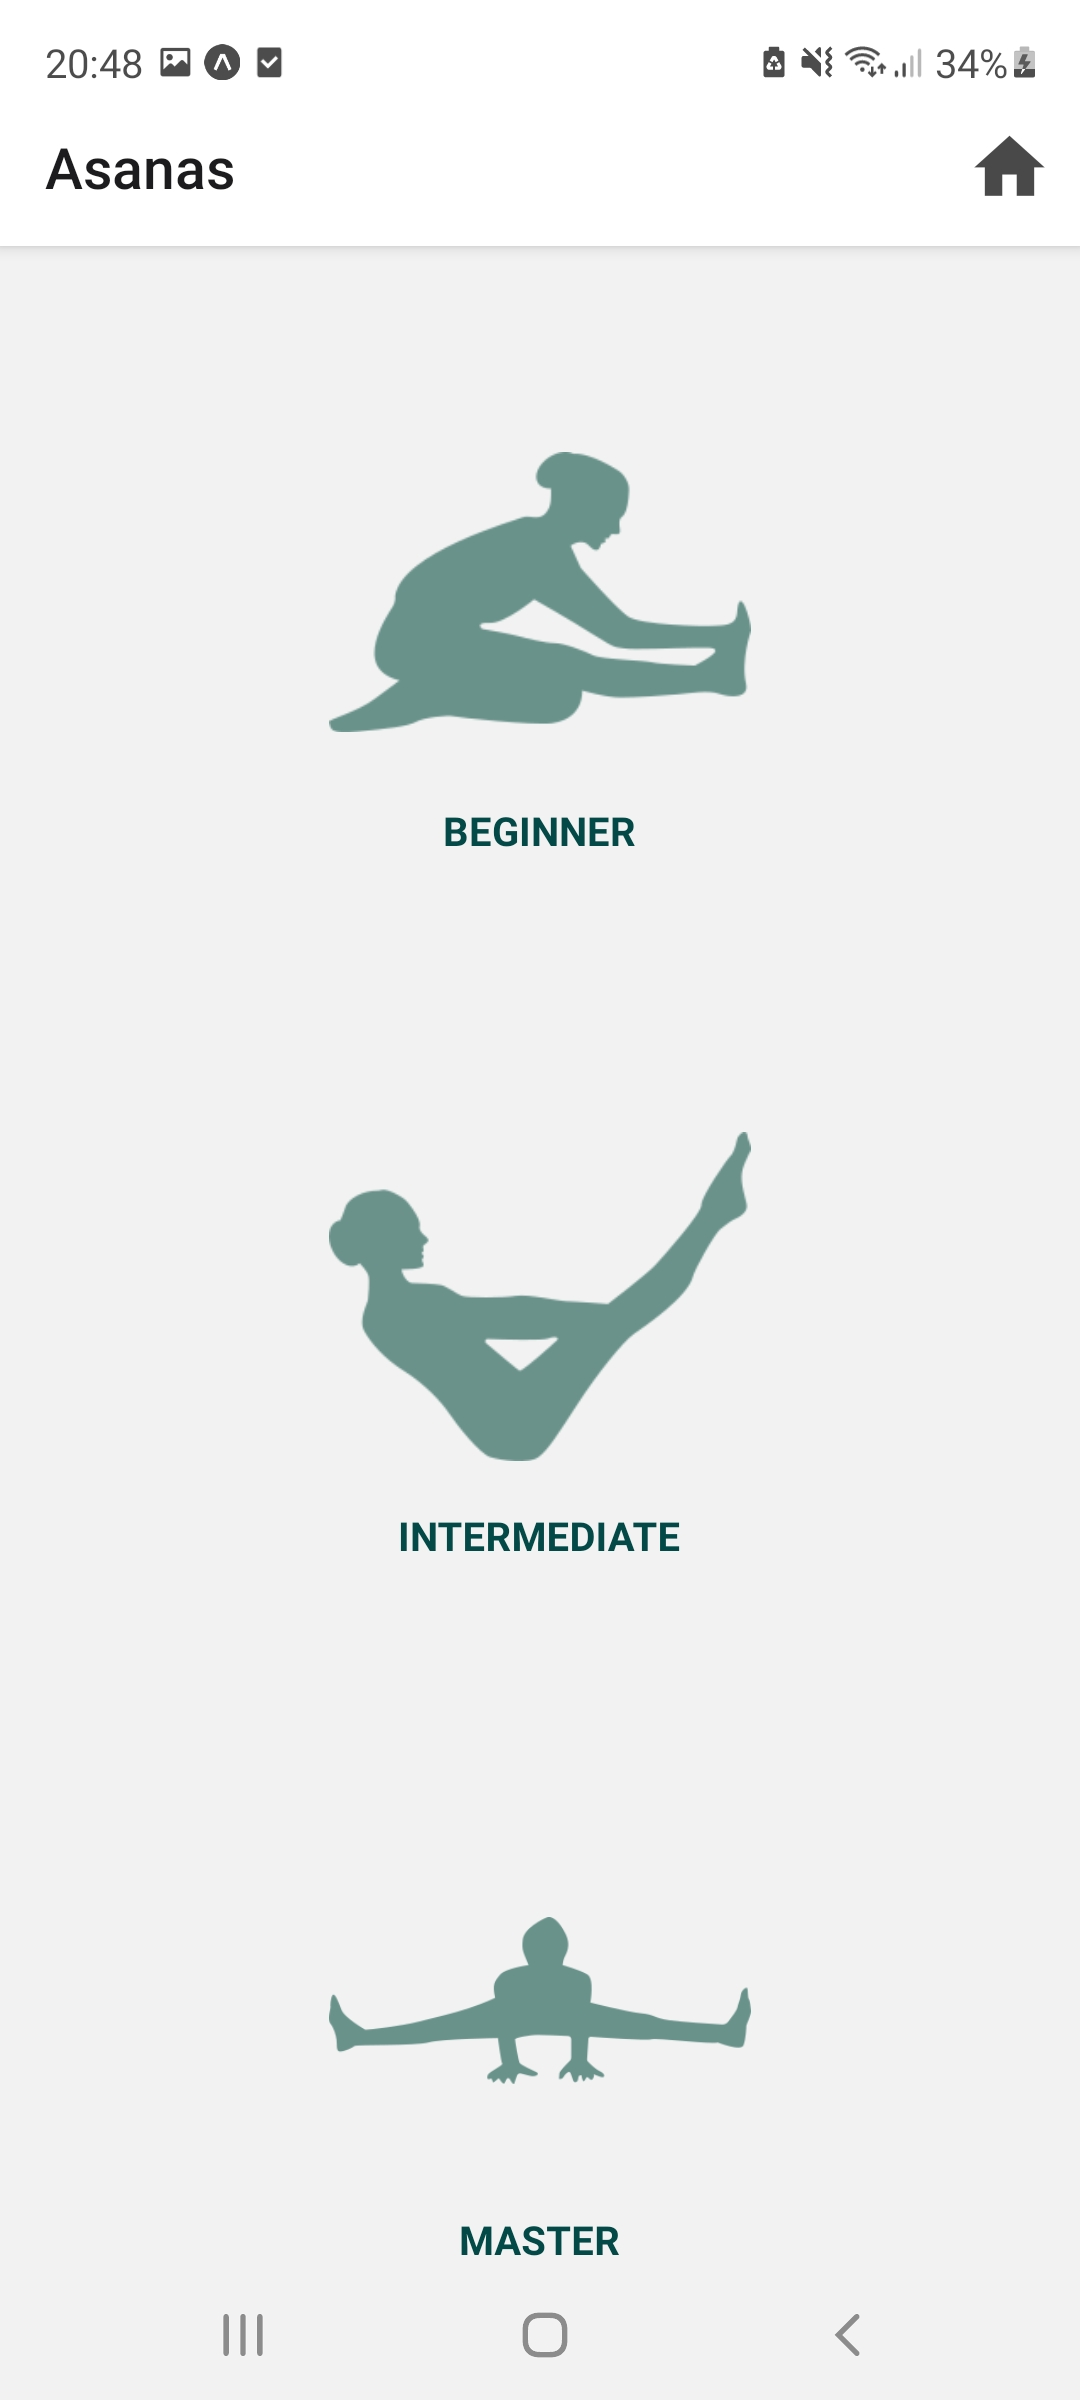
\includegraphics[width=\textwidth]{asanas.jpg}\centering
  \end{minipage}
  \begin{minipage}[b]{0.32\textwidth}
    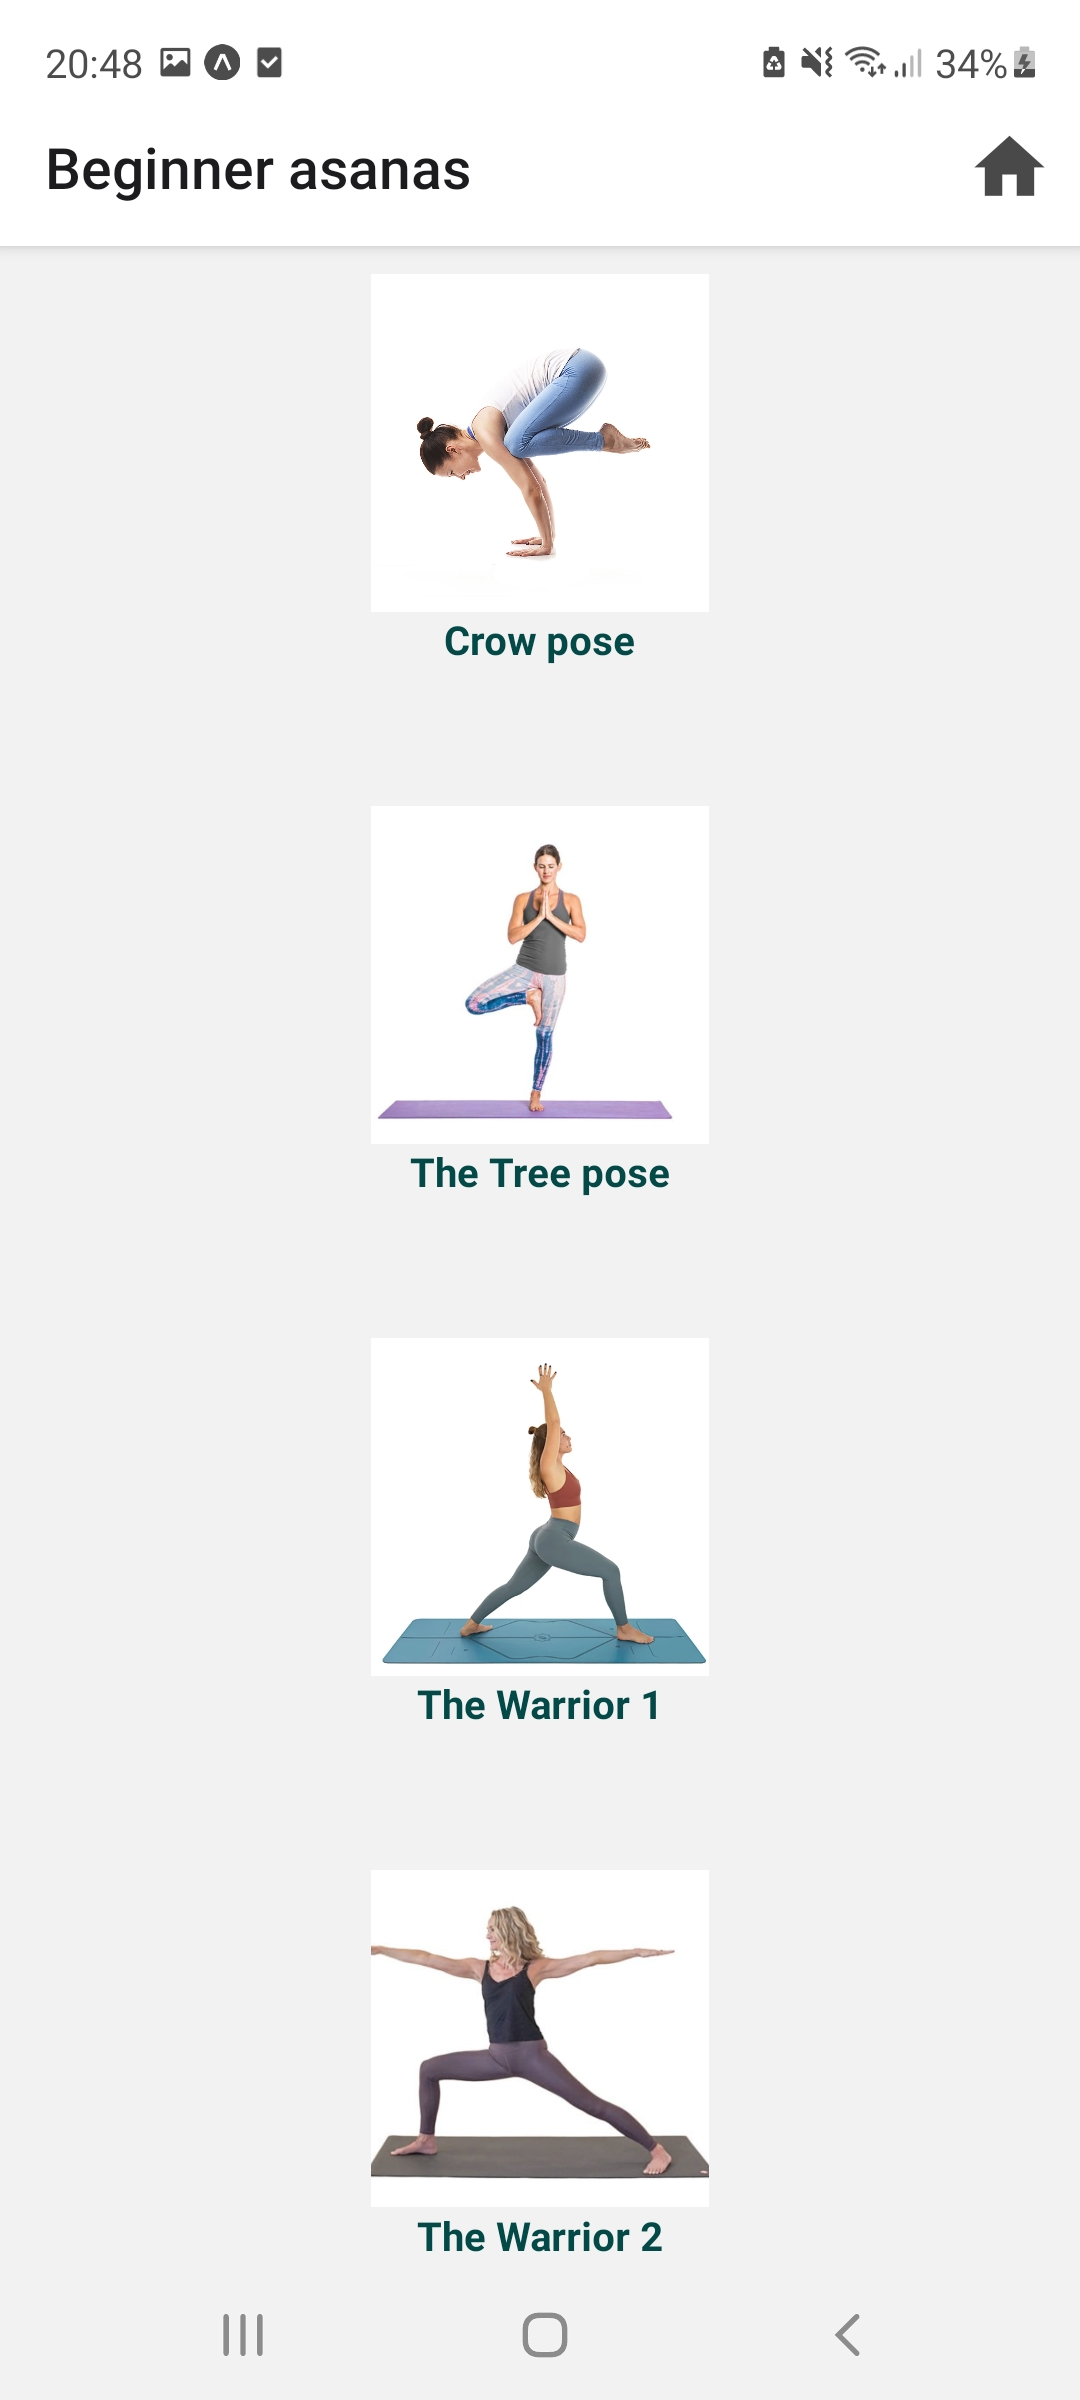
\includegraphics[width=\textwidth]{beginnerasanas.jpg}\centering
  \end{minipage}
    \caption{Podmeni s težavnostmi položajev (levo) in seznam položajev v podmeniju \textit{Begginer} (desno)}
    \label{asana}
    \begin{minipage}[b]{0.32\textwidth}
    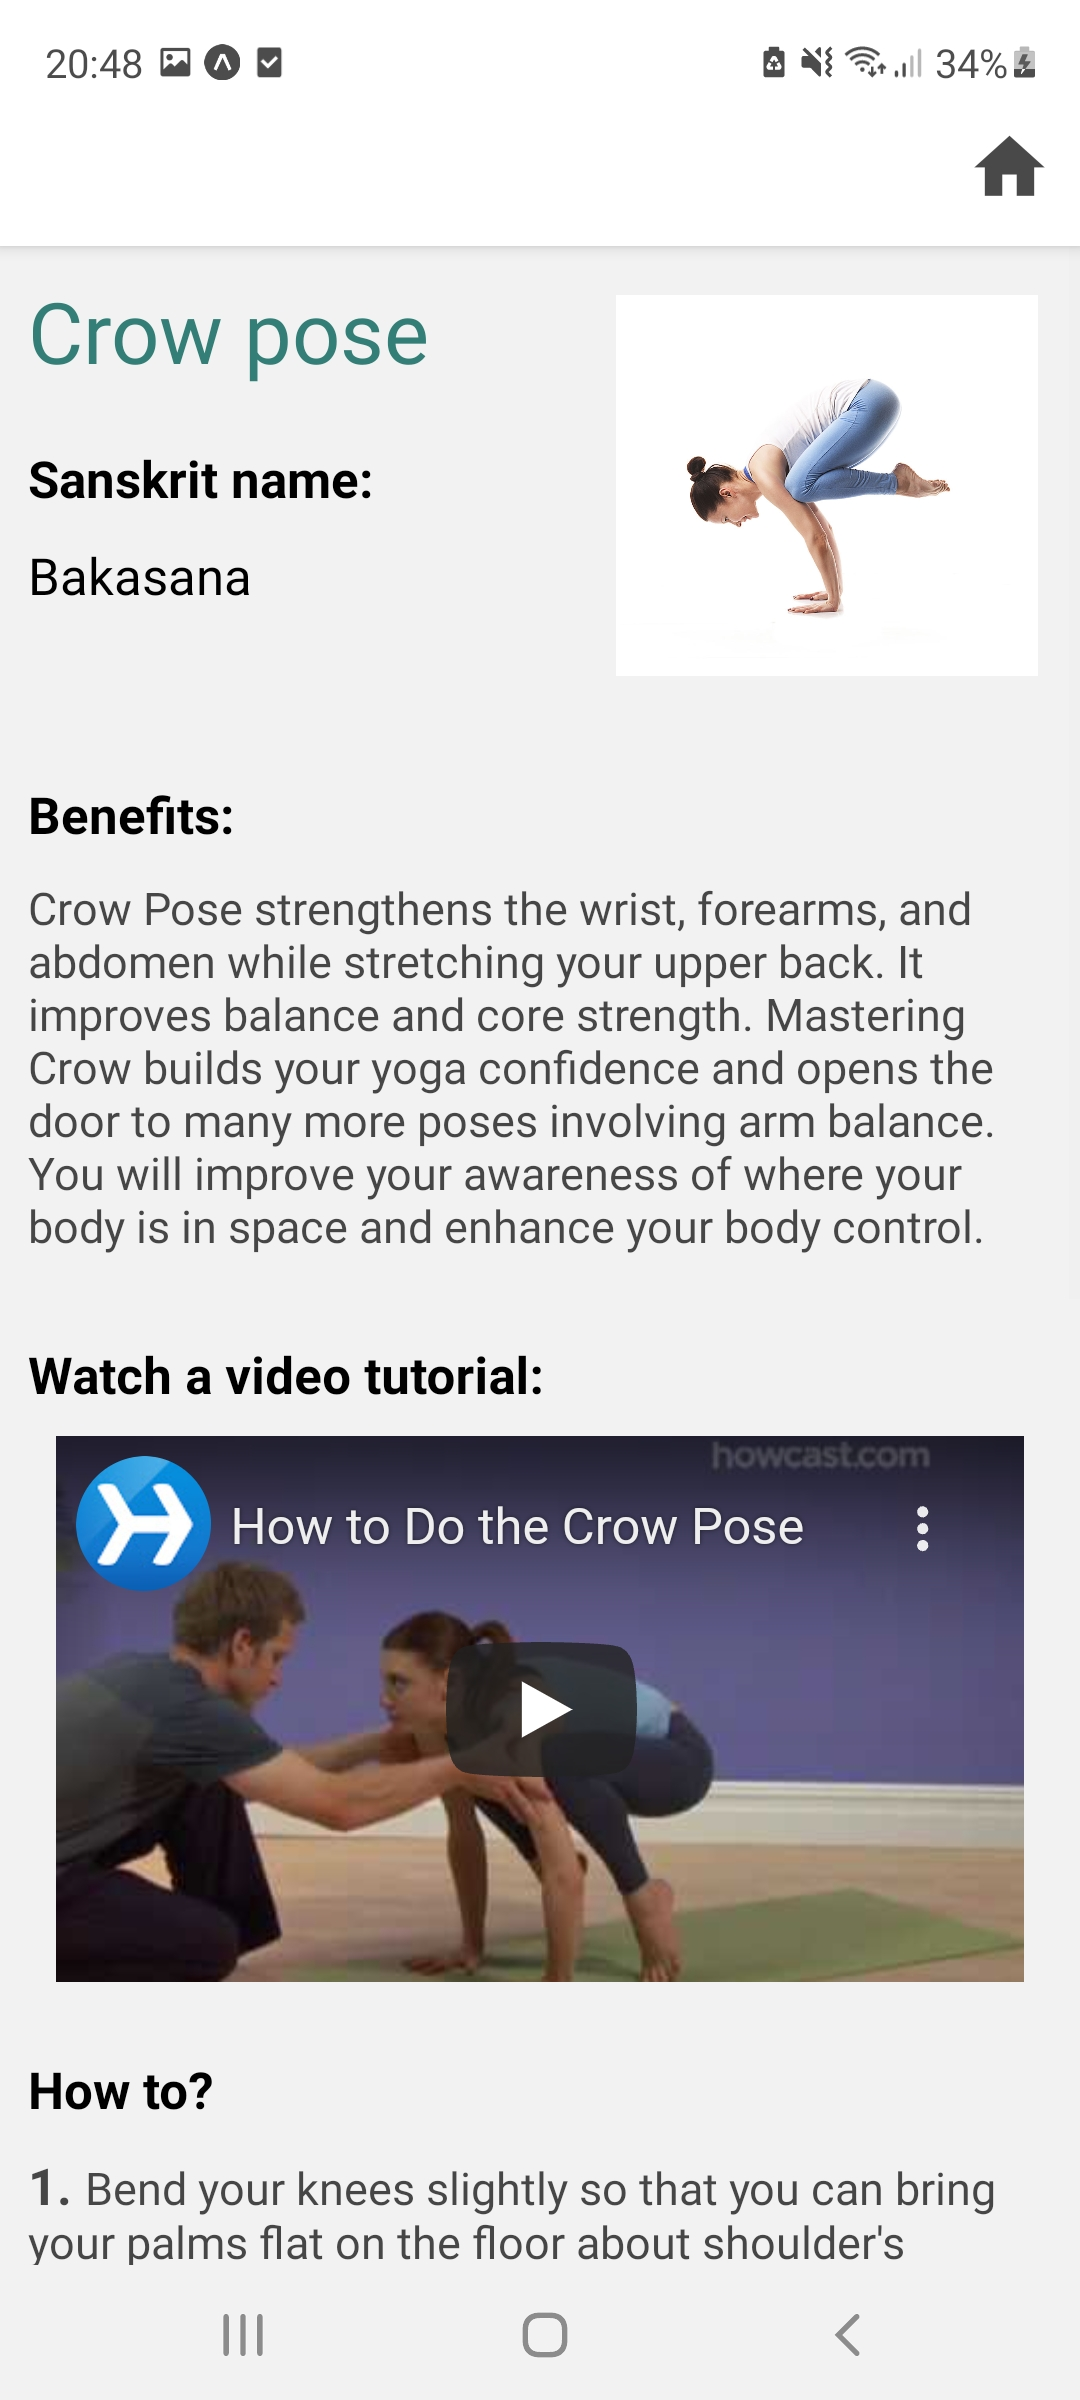
\includegraphics[width=\textwidth]{crowposeasana.jpg}\centering
  \end{minipage}
  \begin{minipage}[b]{0.32\textwidth}
    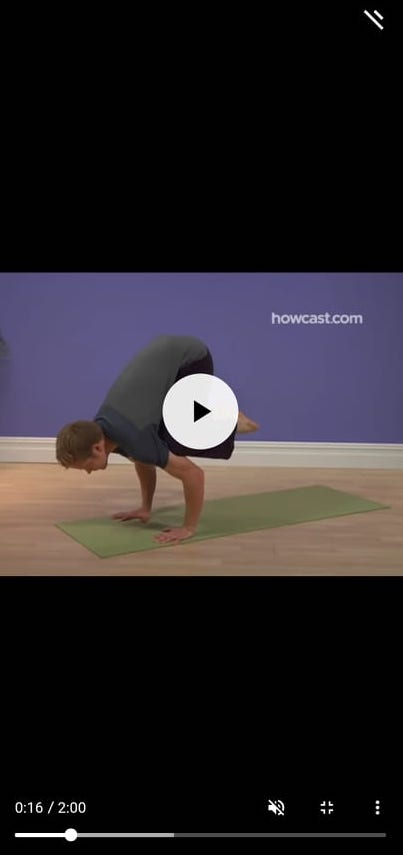
\includegraphics[width=\textwidth]{videoasana.jpg}\centering
  \end{minipage}
  \label{asana2}
  \caption{Stran s podrobnostmi položaja (desno) in predvajanje videa v aplikaciji (desno)}
\end{figure}

Podmeni \textit{Goals} se prav tako razdeli na tri dodatne podstrani, ki predstavljajo tri kategorije, v katerih se lahko uporabnik izboljša in spremlja svoj napredek. Kategorije so: \textit{Splits}, \textit{Backbends} in \textit{Inversions}. Ko si uporabnik izbere eno izmed kategorij, se odpre stran s sedem dnevnim programom različnih videoposnetkov, ki jim uporabnik lahko sledi za lasten napredek, (Slika~\ref{goals}).

\begin{figure}[ht]
\centering
  \begin{minipage}[b]{0.49\textwidth}
    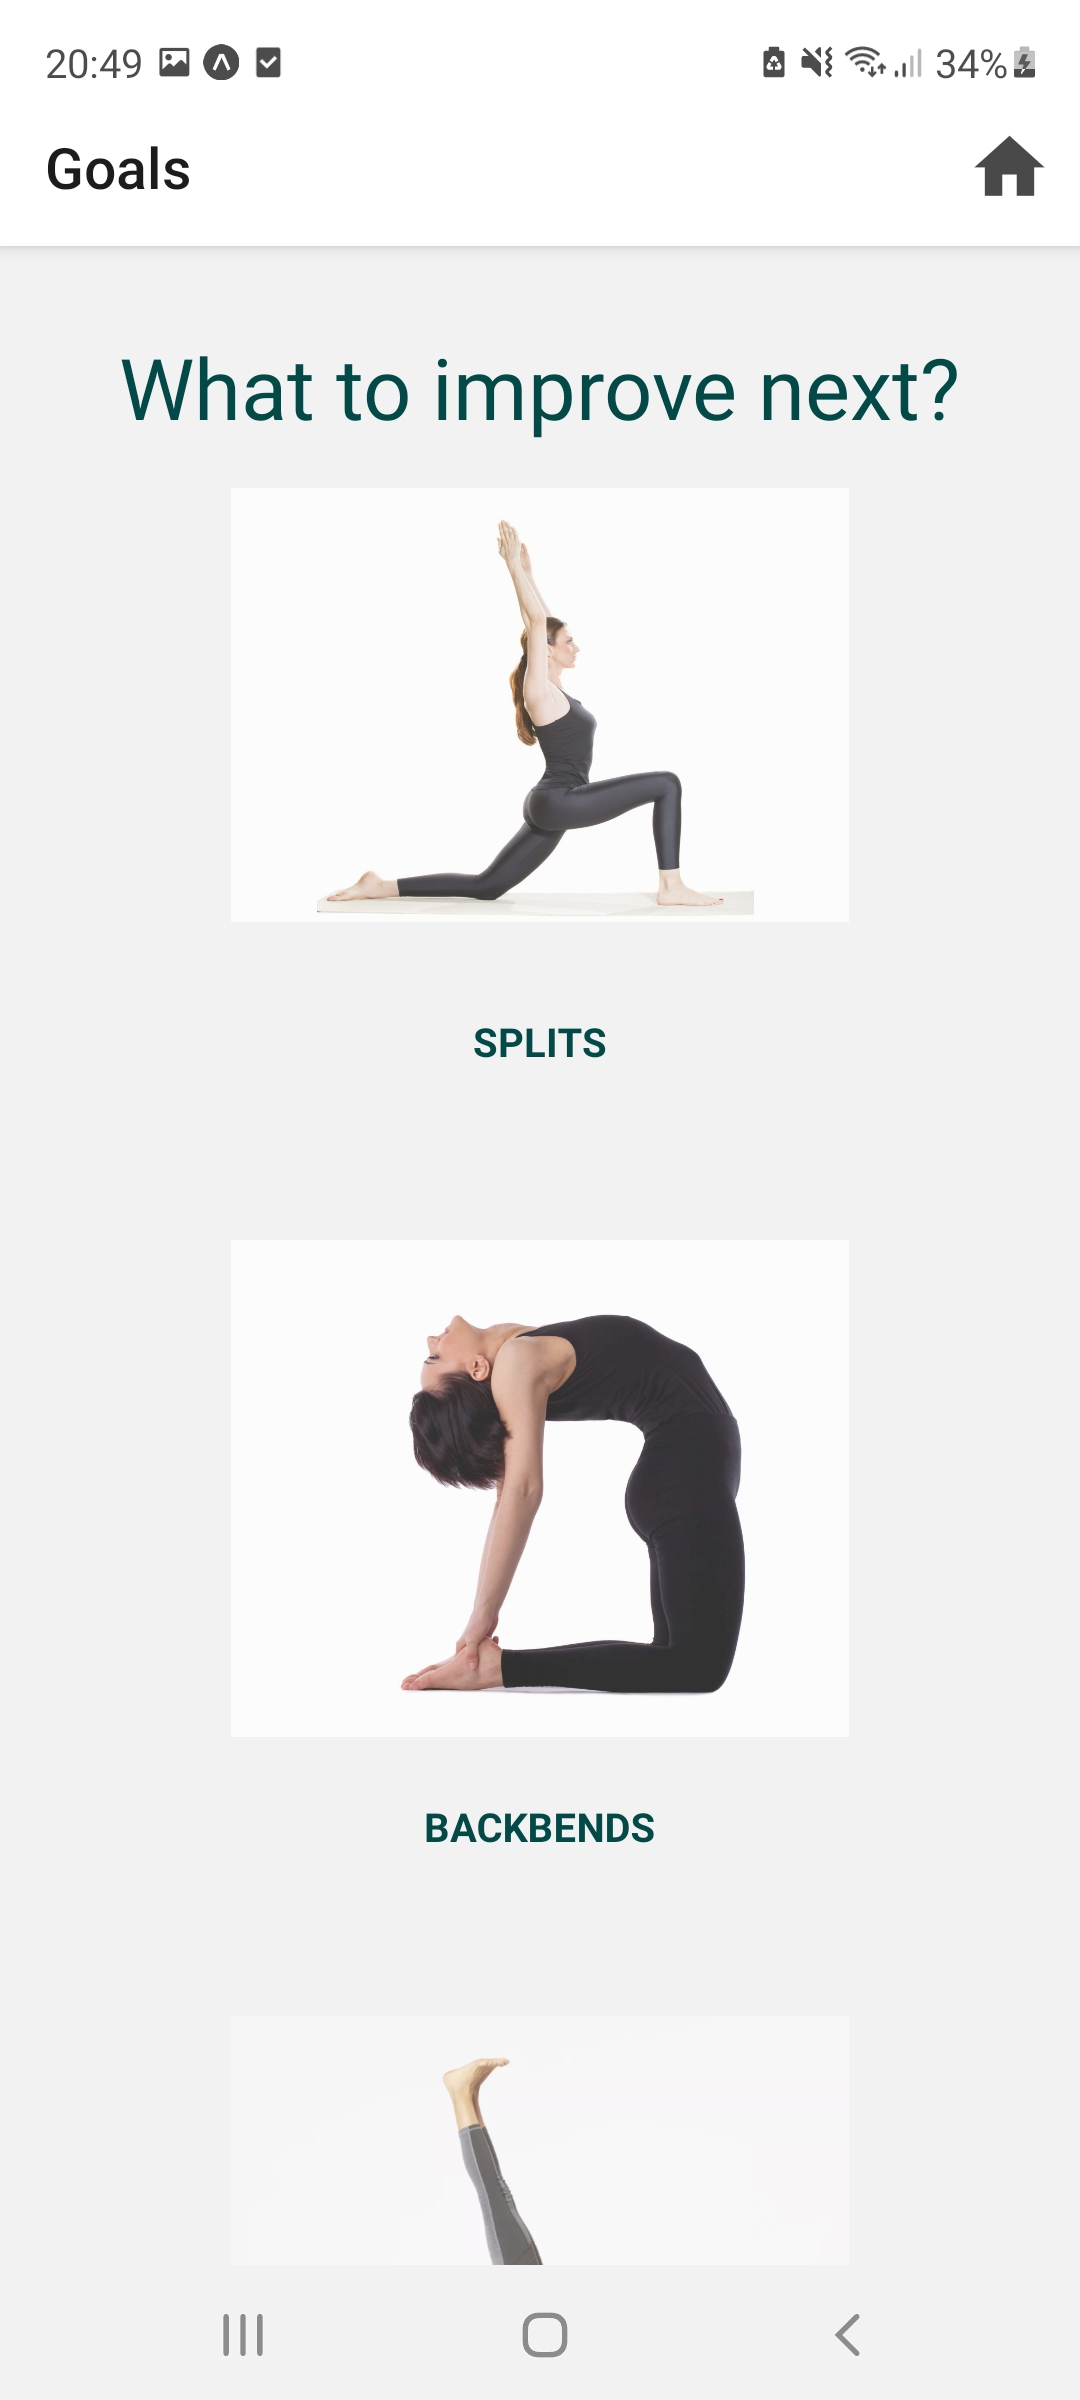
\includegraphics[width=\textwidth]{goals.jpg}\centering
  \end{minipage}
  \begin{minipage}[b]{0.49\textwidth}
    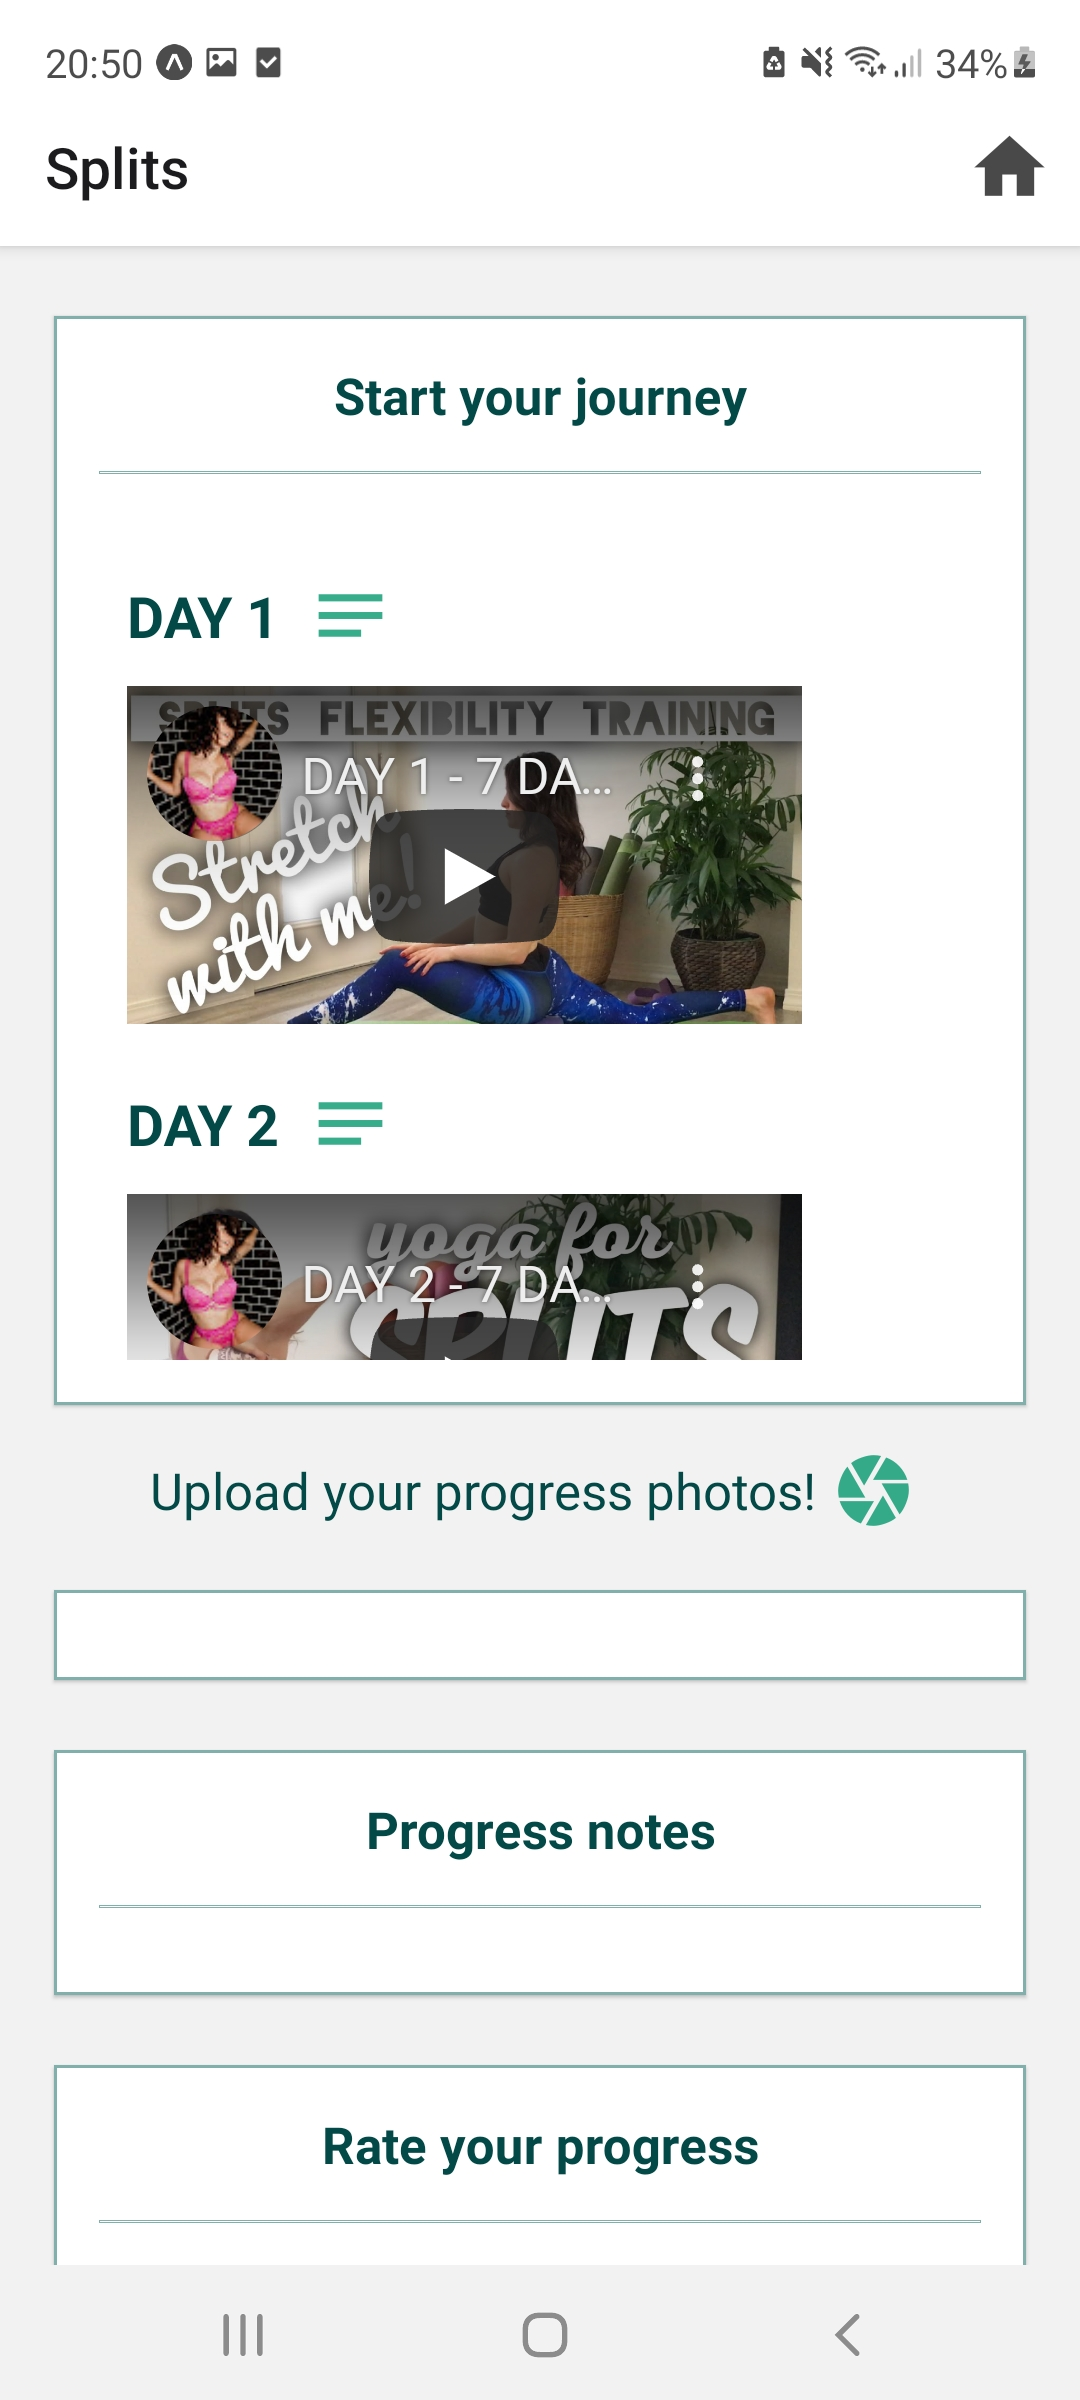
\includegraphics[width=\textwidth]{splits.jpg}\centering
  \end{minipage}
    \caption{Podmeni \textit{Goals} (levo) in podmeni \textit{Splits} (desno).}
    \label{goals}
\end{figure}

Tako kot pri položajih, se tudi tukaj videoposnetek predvaja in odpre neposredno v aplikaciji, brez odpiranja novega okna izven aplikacije. Poleg dneva programa se nahaja ikona za dodajanje zapiska, (Slika~\ref{ikonanotes}). S klikom na ikono lahko uporabnik lahko zapisek vezan na dan v programu, zapisek pa se potem pojavi v razdelku \textit{Progress notes}.

\begin{figure}[htbp]
\centering
  \begin{minipage}[b]{0.55\textwidth}
    
\includegraphics[width=\textwidth]{ikonanotes.jpg}\centering
  \end{minipage}
  \begin{minipage}[b]{0.42\textwidth}
    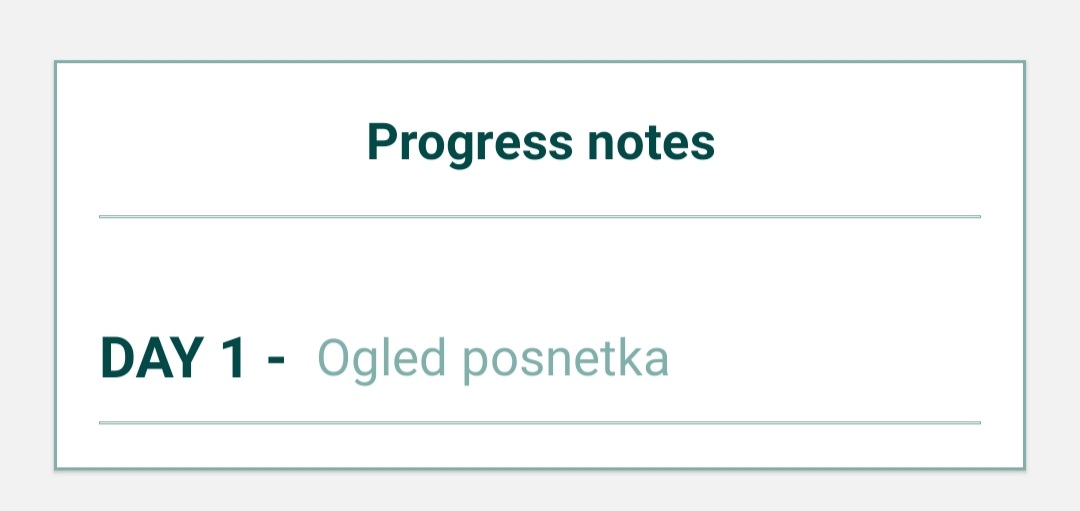
\includegraphics[width=\textwidth]{fullnotes.jpg}\centering
  \end{minipage}
    \caption{Ikona poleg dneva v programu (levo) in razdelek Progress notes v katerem se nahaja seznam zapiskov po dnevih (desno). \\ }
    \label{ikonanotes}
\end{figure}

Pod programom se nahaja možnost dodajanja slik, s katerimi uporabnik lažje sledi napredku, (Slika~\ref{slike}). S klikom na ikono fotoaparata se odpre knjižnica s slikami in videoposnetki na mobilni napravi. 

\begin{figure}[ht]
\centering
  \begin{minipage}[b]{0.56\textwidth}
    
\includegraphics[width=\textwidth]{emptyphoto.jpg}\centering
  \end{minipage}
  \begin{minipage}[b]{0.42\textwidth}
    
\includegraphics[width=\textwidth]{slike.jpg}\centering
  \end{minipage}
    \caption{Razdelek za dodajanje slik (levo) in prikaz naloženih slik v istem razdelku (desno). \\}
    \label{slike}
\end{figure}

Po izboru slike se uporabniku odpre vmesnik za urejanje slike. V vmesniku uporabnik lahko sliko obrača, zrcali ali obreže, (Slika~\ref{crop}). Po končanem urejanju se s klikom na \textit{CROP} slika naloži v mobilno aplikacijo, kjer je vidna v razdelku s slikami. Za ogled slik uporabnik enostavno klikne na sliko, ki se odpre v pregledovalniku slik, med slikami pa se uporabnik premika z drsanjem v levo ali desno.

\begin{figure}[!ht]
\centering
  \begin{minipage}[b]{0.32\textwidth}
    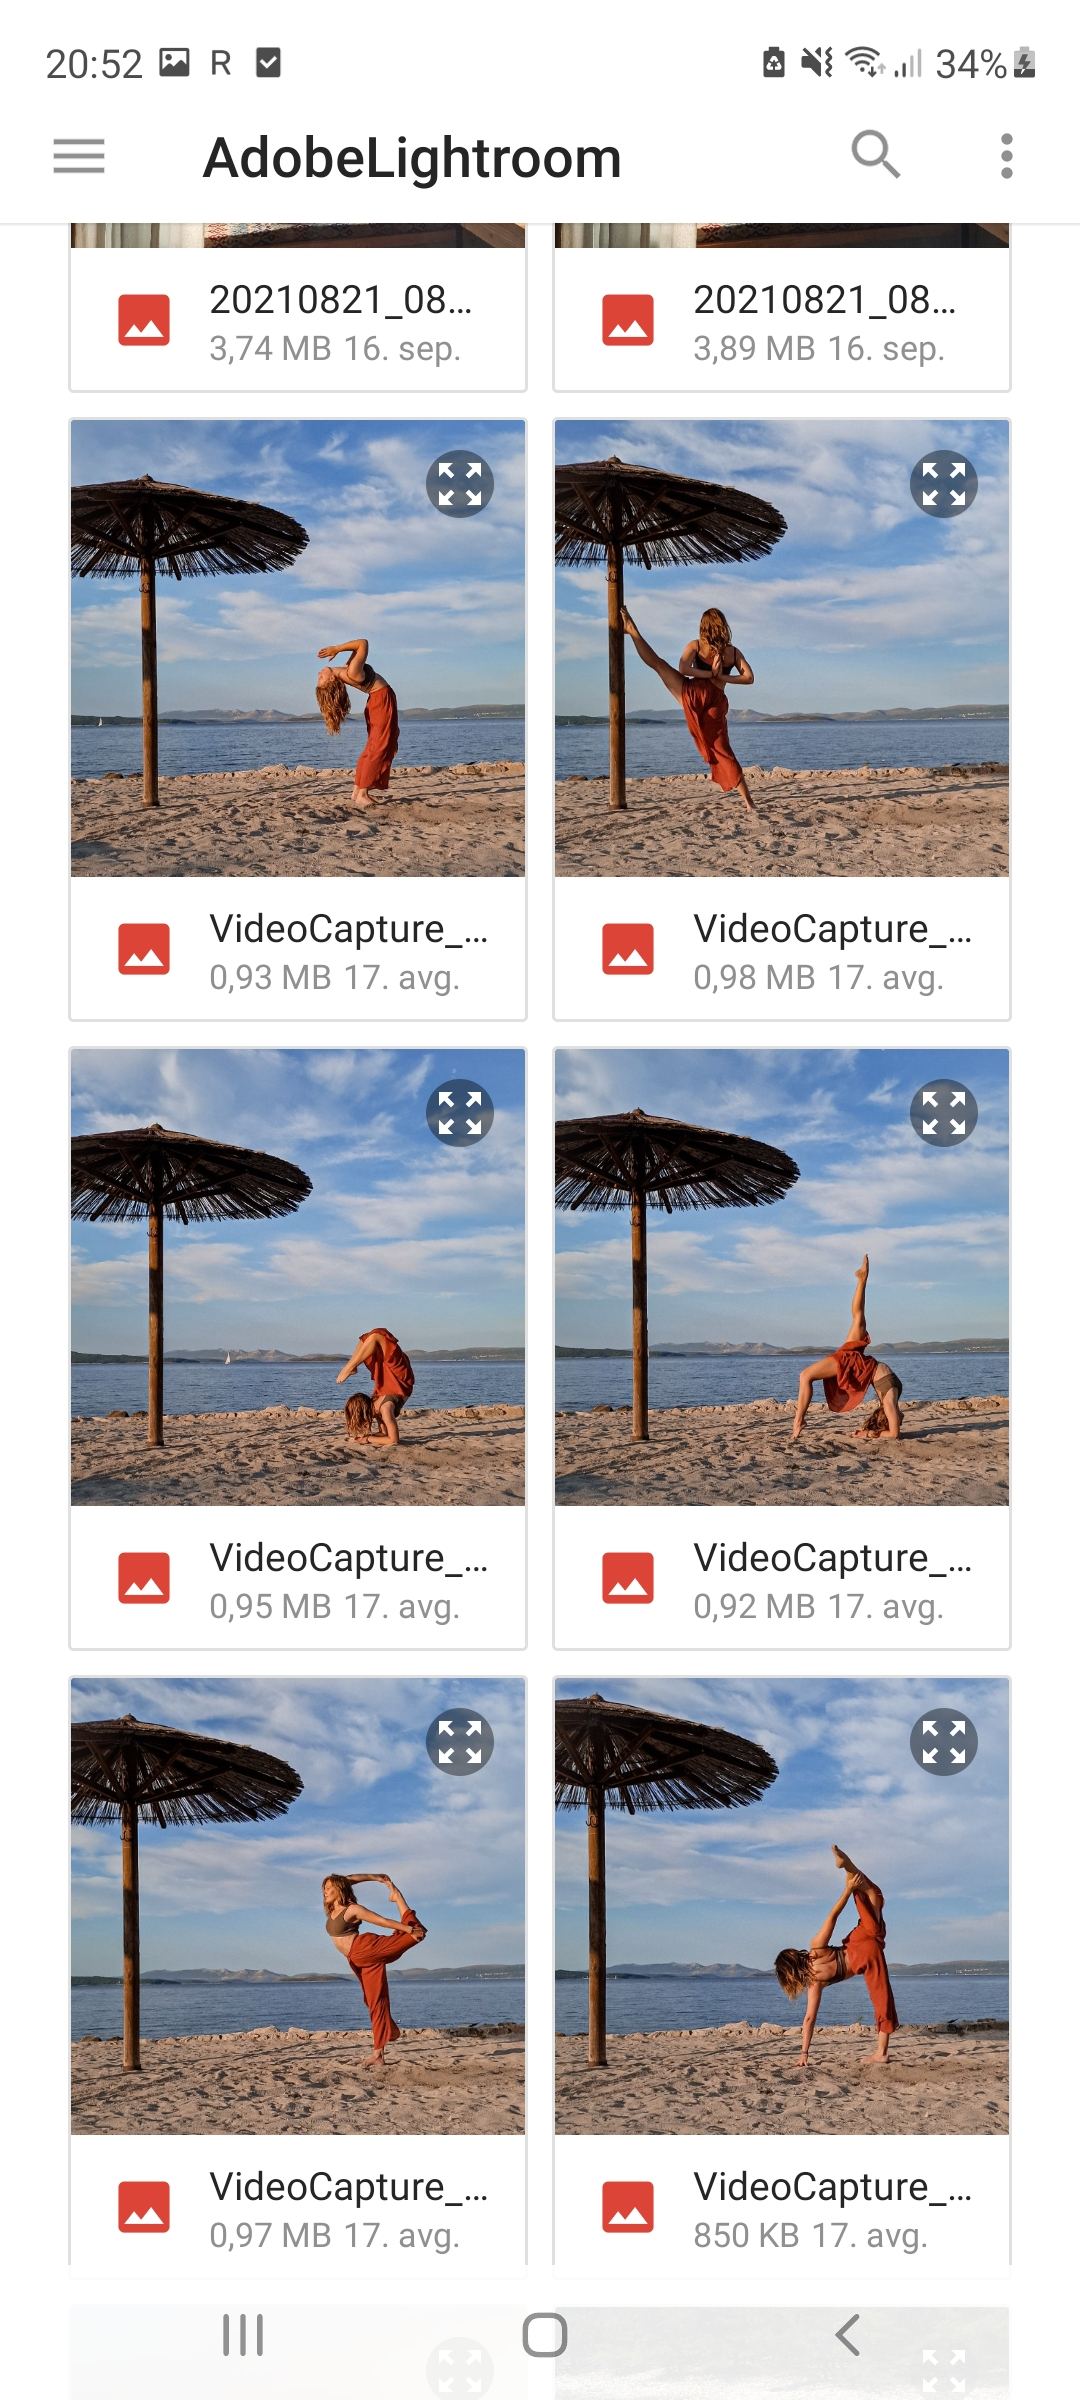
\includegraphics[width=\textwidth]{galerija.jpg}\centering
    \label{menu}
  \end{minipage}
  \begin{minipage}[b]{0.32\textwidth}
    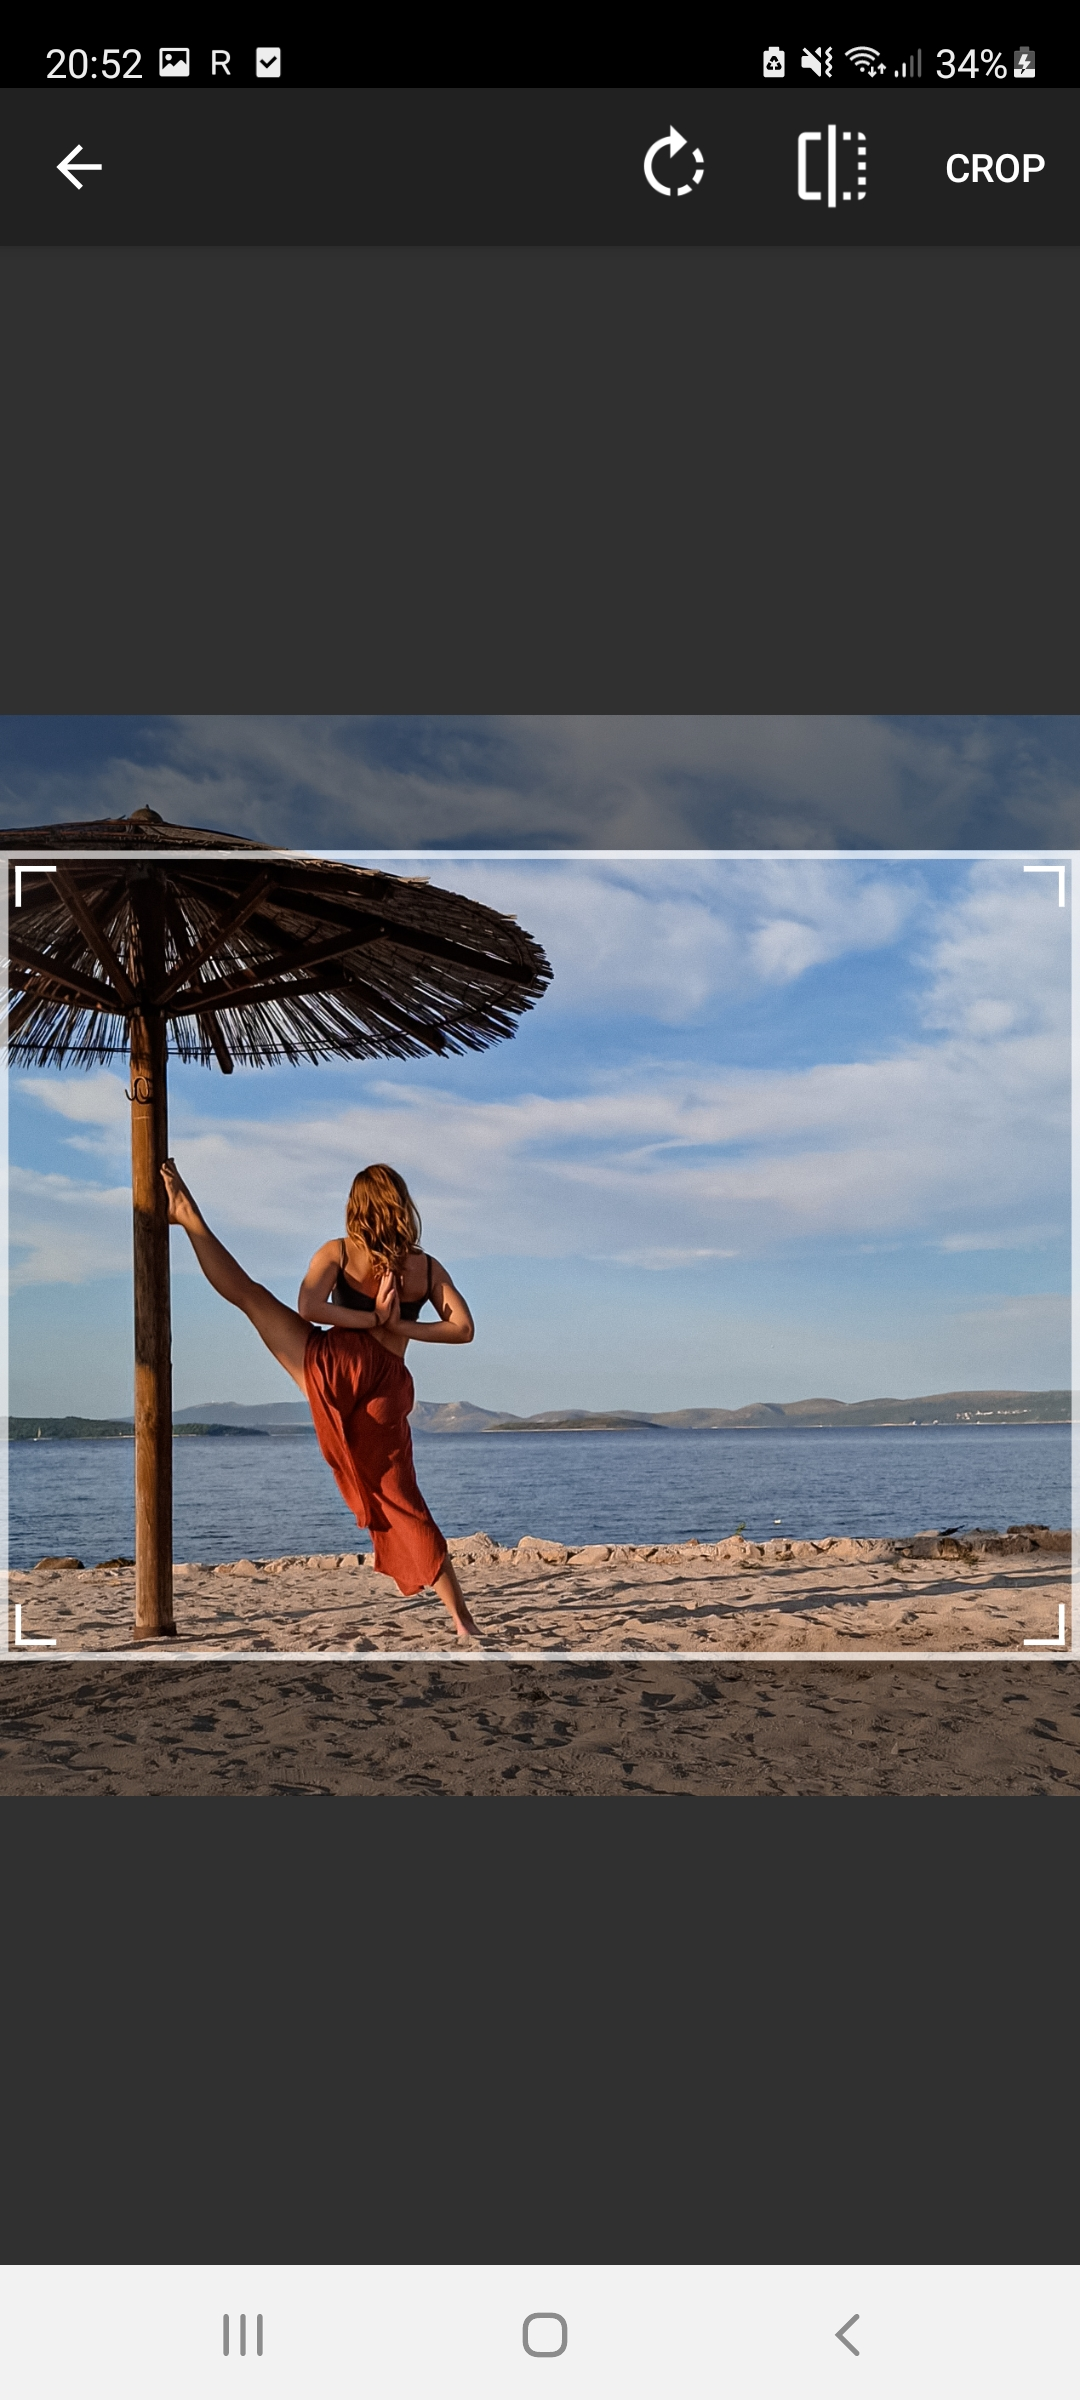
\includegraphics[width=\textwidth]{photocrop.jpg}\centering
  \end{minipage}
  \begin{minipage}[b]{0.32\textwidth}
    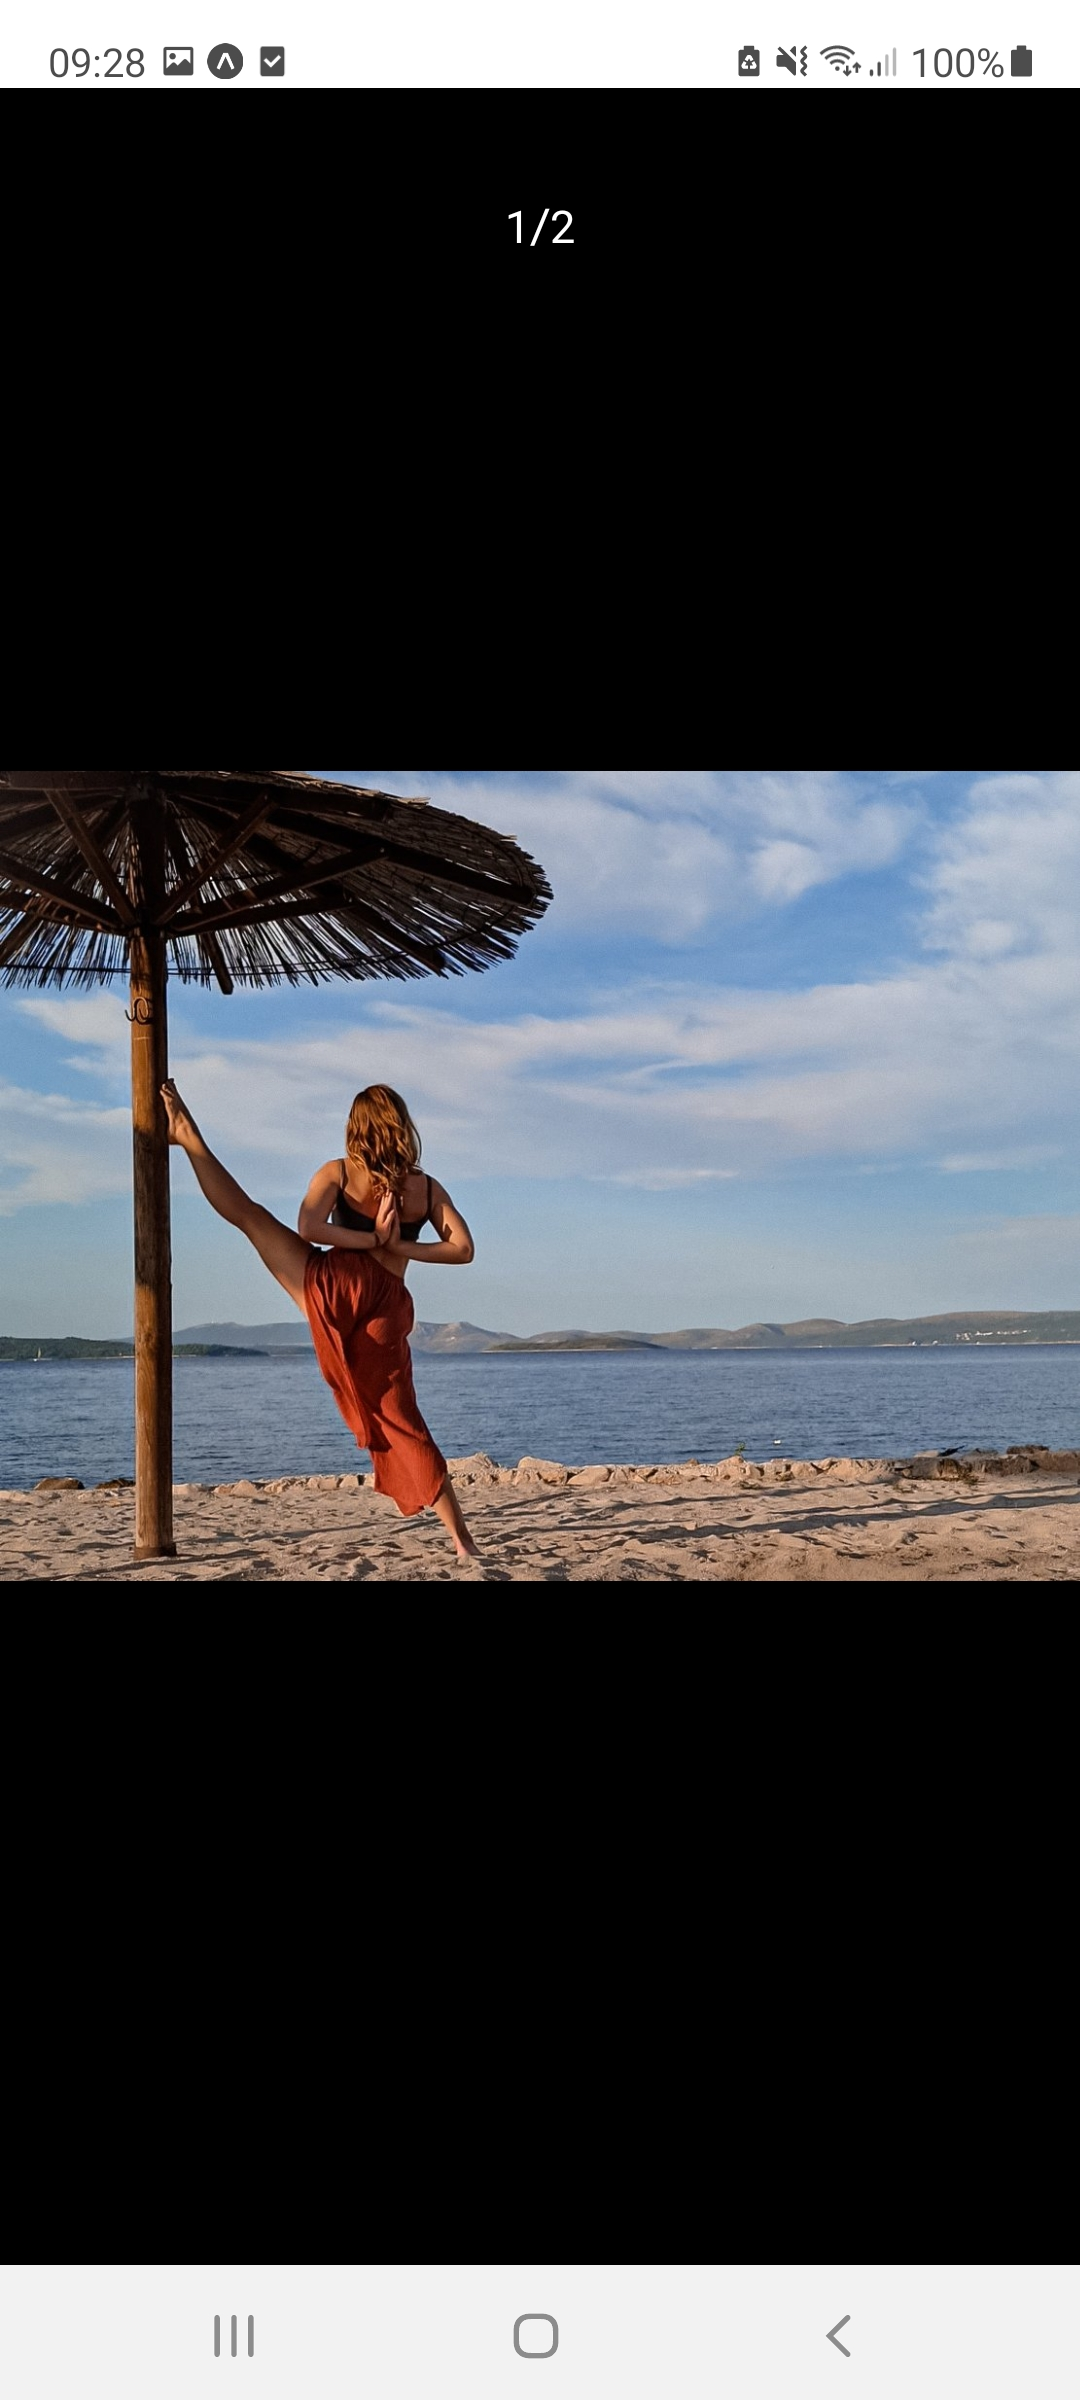
\includegraphics[width=\textwidth]{pregledslik.jpg}\centering
  \end{minipage}
    \caption{Knjižnica slik na napravi (levo), urejevalnik izbrane slike (sredina) in pregledovalnik slik (desno). \\ }
\end{figure}

Uporabnik si lahko pred, med ali po programu poda samooceno, s katero lahko lažje spremlja svoj lasten napredek in kakšen rezultat je dosegel, (Slika~\ref{progress}). S klikom na določeno število zvezdic se le-te obarvajo in izpiše se opis ocene.

\begin{figure}[!ht]
\centering
  \begin{minipage}[b]{0.46\textwidth}
    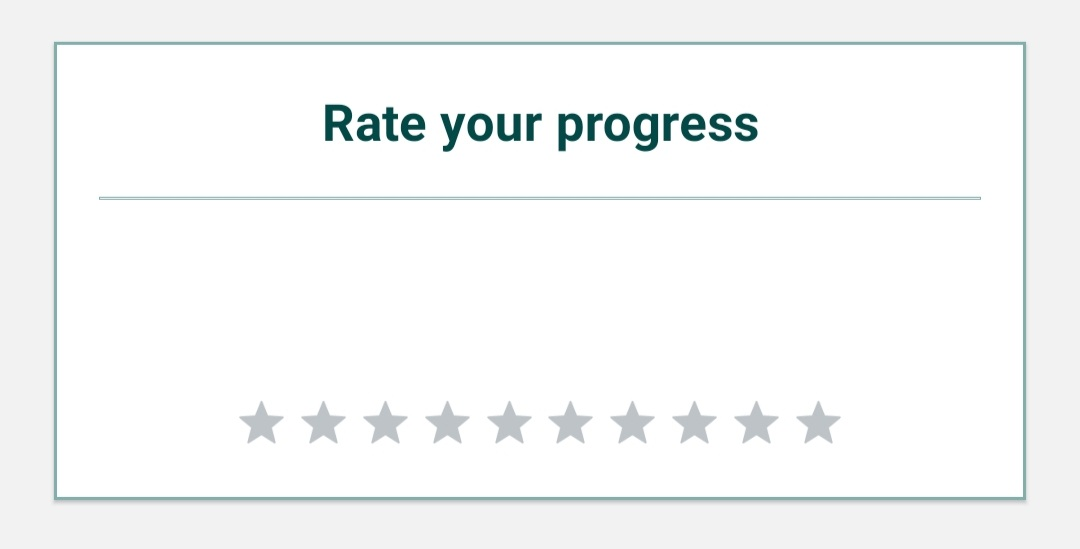
\includegraphics[width=\textwidth]{emptyprogress.jpg}\centering
  \end{minipage}
  \begin{minipage}[b]{0.49\textwidth}
    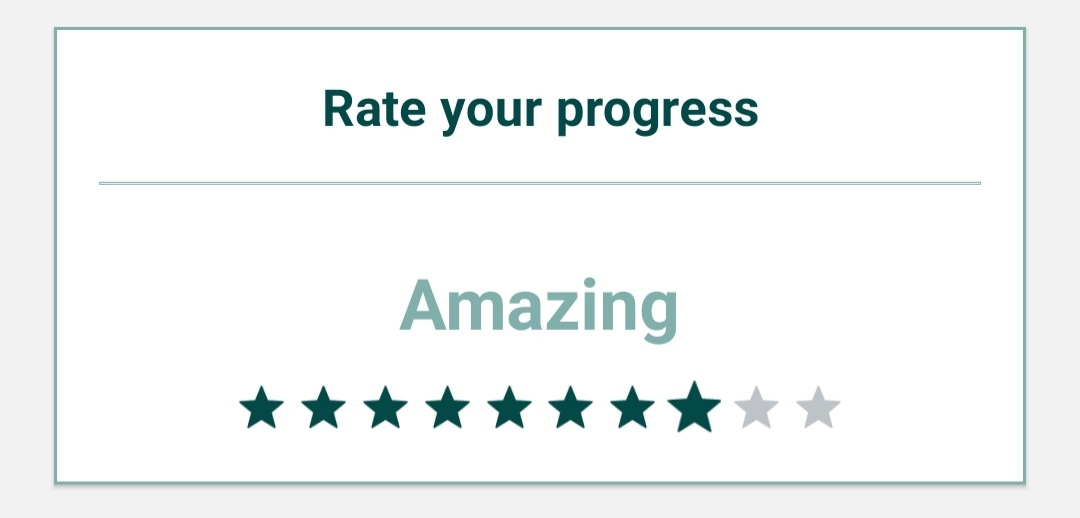
\includegraphics[width=\textwidth]{fullprogress.jpg}\centering
  \end{minipage}
    \caption{Prazen razdelek za podajanje ocene napredka (levo) in podana ocena (desno).}
    \label{progress}
\end{figure}

Podmeni \textit{Notes} ima seznam zapiskov, ki jih je uporabnik ustvaril, ter spodaj desno gumb za dodajanje novega zapiska, (Slika~\ref{zapiski1}). Vsak zapisek v seznamu je razvrščen v ustrezno kategorijo in prikazan z imenom na levi strani vrstice, na desni strani vrstice pa se nahaja ikona koša za smeti, s klikom na katerega lahko uporabnik izbriše zapisek. S klikom na gumb za dodajanje zapiska, se uporabniku odpre forma za vnos naslova zapiska in okno za vnos vsebine zapiska. Pod oknom za vsebino se nahajata še dva gumba, levo gumb \textit{Back}, ki uporabnika vrne v seznam zapiskov in desno gumb \textit{Save}, ki omogoča shranitev zapiska.

\begin{figure}[!htbp]
\centering
  \begin{minipage}[b]{0.41\textwidth}
    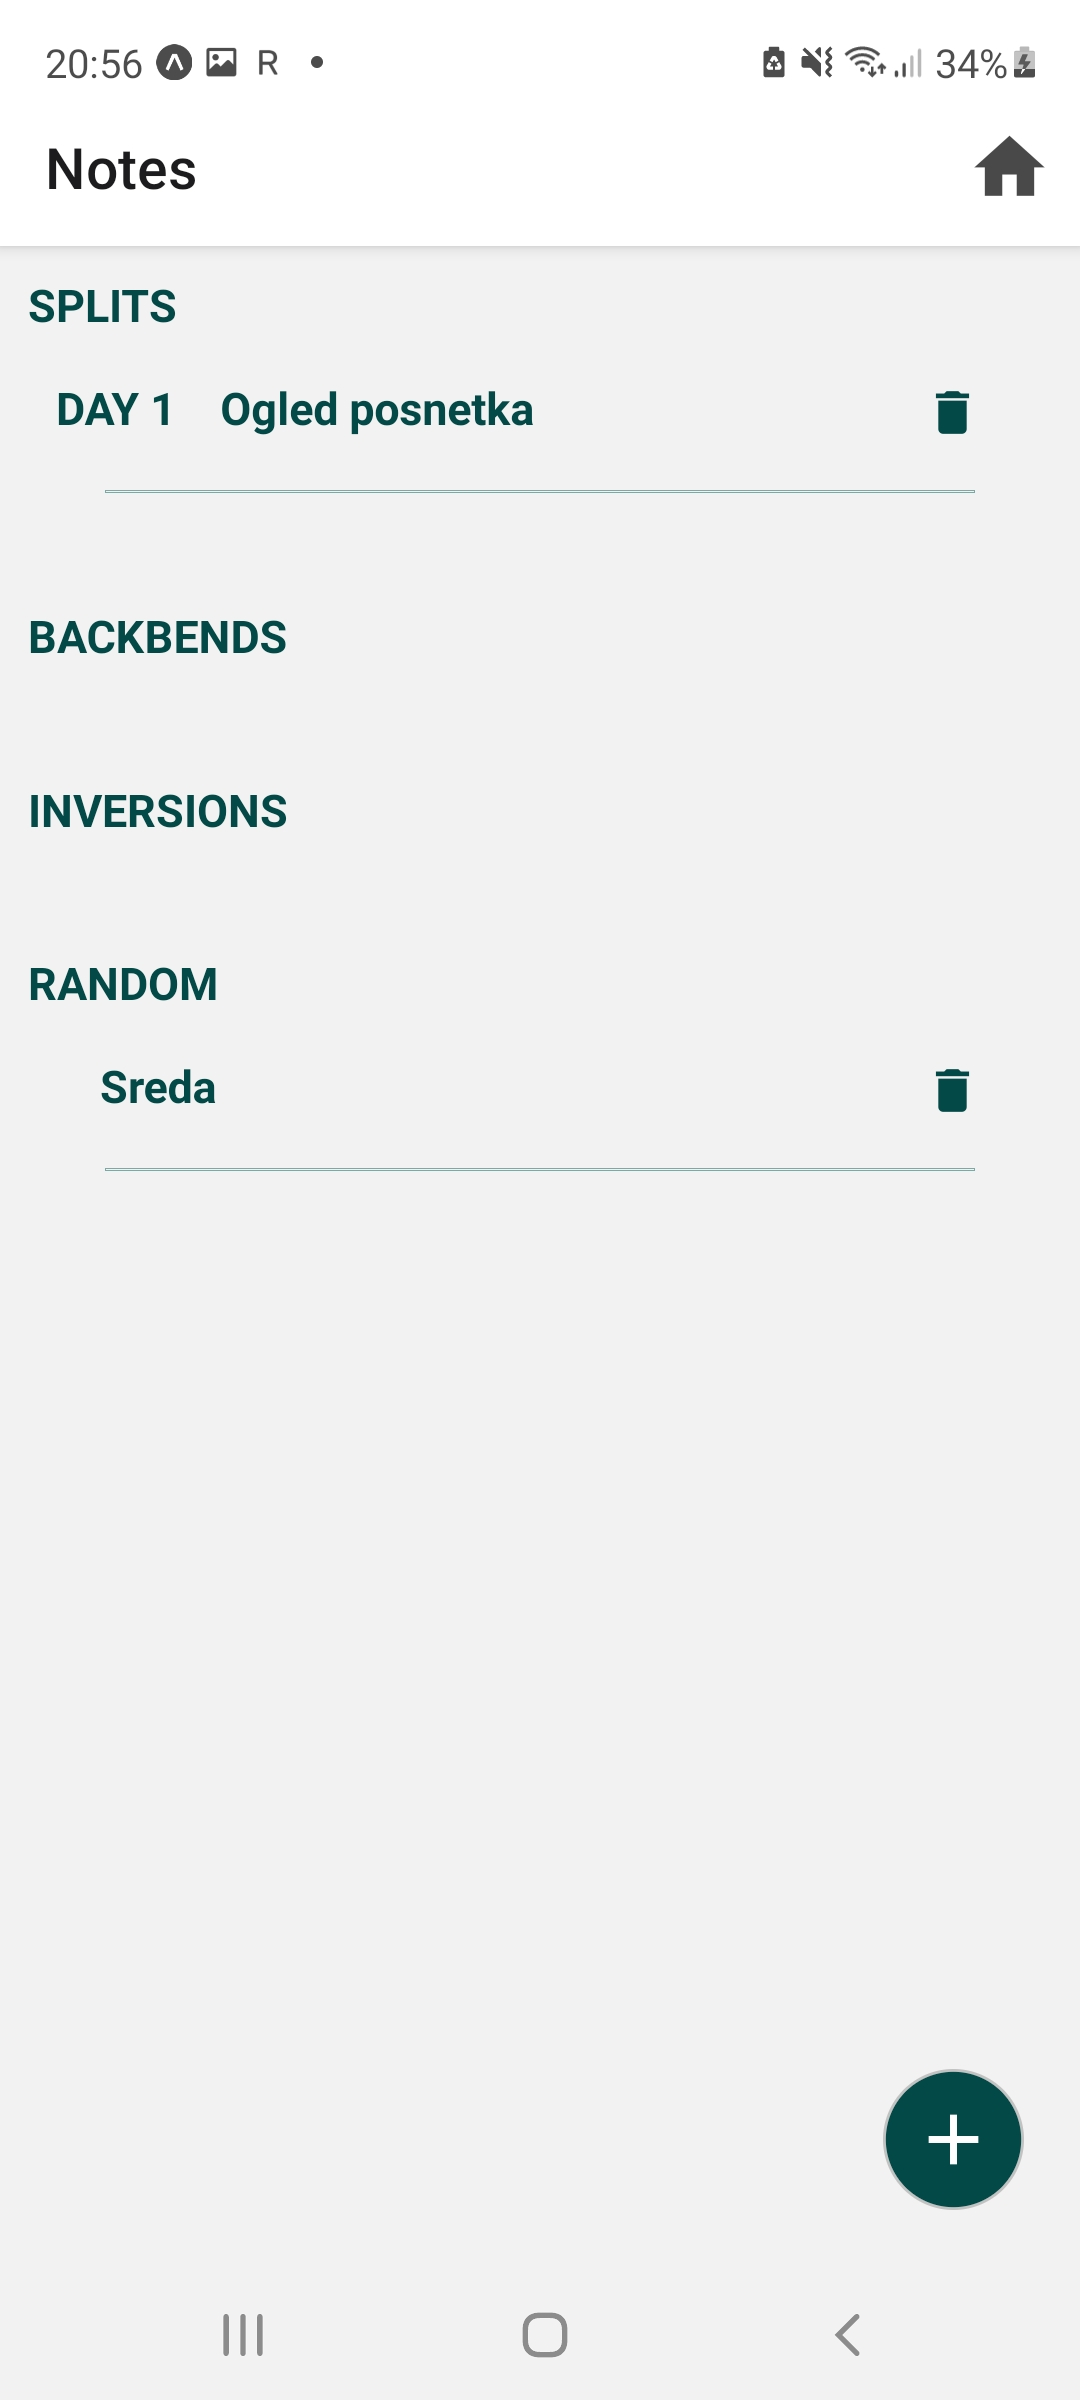
\includegraphics[width=\textwidth]{random.jpg}\centering
  \end{minipage}
  \begin{minipage}[b]{0.41\textwidth}
    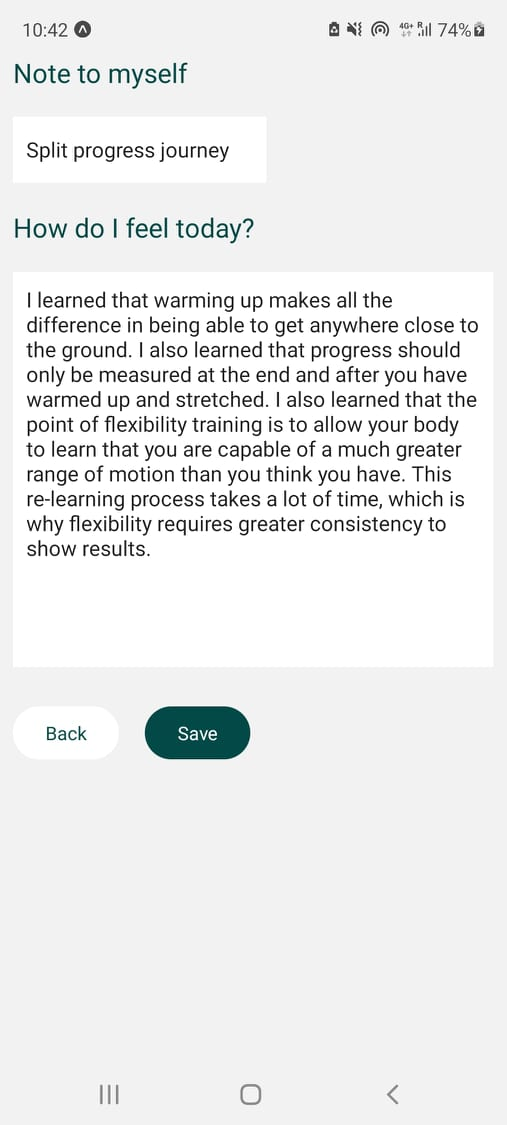
\includegraphics[width=\textwidth]{ustvarjanjezapiska.jpg}\centering
  \end{minipage}
    \caption{seznam zapiskov (levo) in forma z vneseno vsebino zapiska (desno).}
    \label{zapiski1}
\end{figure}

Po shranitvi zapiska je uporabnik samodejno preusmerjen nazaj na seznam zapiskov. 
S klikom na izbrani zapisek se odpre stran z naslovom zapiska, datumom, kdaj je bil zapisek ustvarjen in zapisano besedilo uporabnika, (Slika~\ref{zapiski2}).

\begin{figure}[!ht]
\centering
  \begin{minipage}[b]{0.45\textwidth}
    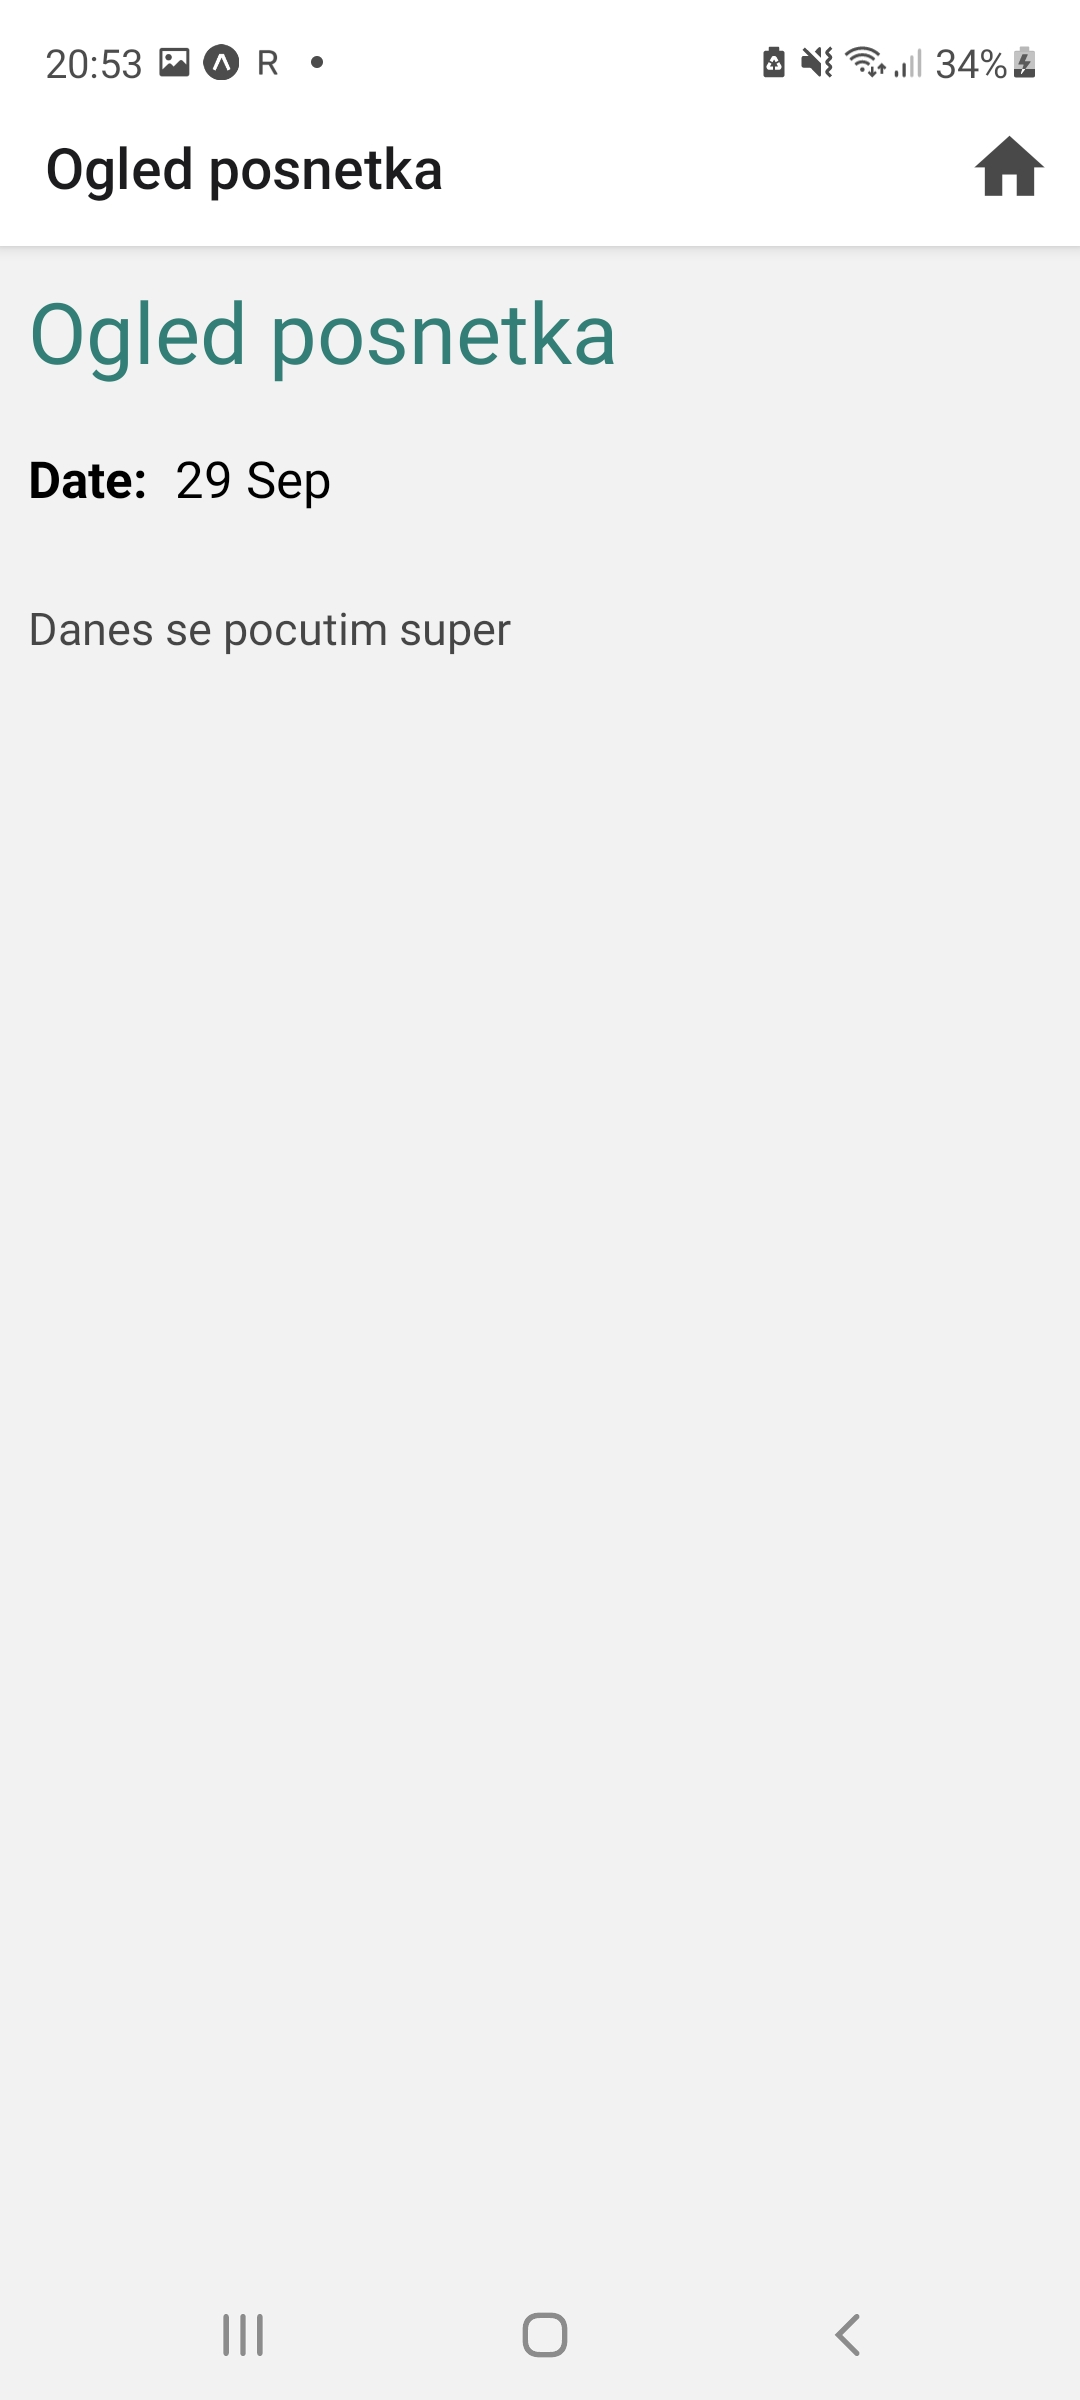
\includegraphics[width=\textwidth]{ogledzapiska.jpg}\centering
  \end{minipage}
    \caption{Prikaz strani z ogledom podrobnosti zapiska (desno).}
    \label{zapiski2}
\end{figure}

Za odjavo iz aplikacije lahko uporabnik v vsakem od podmenijev klikne gumb  \textit{Home}  (ikona hiške zgoraj desno), ki ga preusmeri v glavni meni, kjer se na istem mestu nahaja gumb za odjavo.

\chapter{Sklepne ugotovitve}
\label{stroka}

V sklopu diplomske naloge smo raziskovali področje mobilnih aplikacij namenjenih učenju joge in jih primerjali z našo aplikacijo. Ugotovili smo, da imajo nak skupnih funkcionalnosti, vsaka pa ima tudi svojo dodano vrednost, ki privablja različne tipe uporabnikov. V diplomskem delu smo opisali katera orodja in tehnologije so bile uporabljene pri razvoju mobilne aplikacije, opisali smo korake načrtovanja ter predstavili mobilno aplikacijo. Na koncu pa smo opisali še možen načrt za nadaljni razvoj. 

Menimo, da smo v diplomskem delu prišli do cilja, ki smo si ga zastavili, imamo pa s trenutno verzijo aplikacije še kar nekaj možnega prostora za razvoj in nadgradnjo. Veliko časa smo namenili zbiranju in prepisovanju podatkov, saj je številen nabor asan pomemben za boljšo uporabniško izkušnjo. Prav tako smo veliko časa namenili raziskovanju in načrtovanju razvoja aplikacije, da smo izbrali najbolj primerna orodja in tehnologije za sam razvoj. Z izdelavo prototipa nismo imeli težav, saj smo na tem področju imeli že kar nekaj izkušenj. Največji izziv pri razvoju pa nam je predstavljala prijava in avtentikacija uporabnika. 

Končen rezultat diplomske naloge je mobilna aplikacija, ki uporabnikom omogoča učenje jogijskih položajev, učenje in izboljšanje osebnih ciljev, nalaganje slik za lažje spremljanje napredka in ustvarjanje zapiskov, kar zaokroži celoten učni proces, ki smo ga želeli ustvariti s to aplikacijo.


\section{Ideje za nadaljni razvoj}
Prva ideja za nadaljnji razvoj je razširitev baze podatkov, s katero bi imeli uporabniki dostop do več vsebine za učenje.

Naslednja možna nadgradnja bi lahko bil bolj personaliziran program za osebni napredek uporabnika, tako da bi se posnetki in programi ustvarjali samodejno glede na podano oceno uporabnika. Na primer, v kolikor bi uporabnik podal oceno svojega napredka 6 in ocene nekaj časa ne bi spreminjal, bi mu aplikacija tekom časa ponudila nov program, katerumu bi uporabnik sledil za napredek. 

Prav tako bi ena izmed možnih nadgradenj bila povezovanje uporabnikov z drugimi uporabniki, tako da bi si lahko ogledali profil drugega uporabnika in preverili njegov napredek, kar bi morda nekatere uporabnike še dodatno motiviralo. 

Zadnja ideja pa je razširitev uporabniških profilov, s katerim bi že obstoječim učiteljem omogočili sestavljanje in objavljanje programov, katerim bi potem drugi uporabniki lahko sledili.


\clearpage
\addcontentsline{toc}{chapter}{Literatura}
\bibliographystyle{plain}
\bibliography{literatura}

\end{document}

